% PhD checklist: https://www.mnf.uzh.ch/en/studium/phd/checkliste-fuer-doktorierende.html
% UZH CMS wiki https://wiki.physik.uzh.ch/cms/newcomers:gettingstarted#phd_students
\RequirePackage{fix-cm} % against warnings for \fontsize
%\documentclass[a4paper,11pt]{book}
\documentclass[a4paper,11pt,usegeometry]{scrreprt} % scrreprt = KOMA script
\usepackage[T1]{fontenc} % load before inputenc
\usepackage[utf8]{inputenc}
\usepackage{tikz}
\usepackage{setspace}
\usepackage{geometry}
\usepackage{ragged2e}
\usepackage{hyperref}
%math packages:
\usepackage{amsmath}
\usepackage{amsfonts}
\usepackage{amssymb}
%graphics packages
\usepackage{xcolor}
\usepackage{graphicx}% Include figure files
\usepackage{epstopdf}
\usepackage{color}
\usepackage{dcolumn}% Align table columns on decimal point
\usepackage{bm}% bold math
\usepackage{ascii}
 \usepackage{longtable}
%\usepackage[colorinlistoftodos]{todonotes}
\usepackage{listings}
\usepackage{pdflscape} %need for rotating PDFs
\usepackage{rotating}
%bibliografi:
\usepackage[inkscapelatex=false]{svg}
\usepackage[backend=biber, bibencoding=utf8,sorting=none]{biblatex}
%\usepackage{csquotes} %not needed, I think. 
%\usepackage[backend=biber, bibencoding=utf8]{biblatex}
\addbibresource{./bibliography/biblio.bib}
\DeclareSourcemap{
 \maps[datatype=bibtex,overwrite=true]{
  \map{
    \step[fieldsource=Collaboration, final=true]
    \step[fieldset=usera, origfieldval, final=true]
  }
 }
}

\renewbibmacro*{author}{%
  \iffieldundef{usera}{%
    \printnames{author}%
  }{%
      \printnames{author} (\printfield{usera})%
  }%
}%

%\usepackage[]{tocbibind}%Add bib to table of contents
%\usepackage{appendix}

%\usepackage{multicol}
\usepackage{multirow}
\usepackage{comment}
\usepackage{relsize}
%\usepackage{gensymb}
\usepackage{float}
%\usepackage{fixltx2e}
\usepackage{textcomp}
\usepackage{hyperref}
\usepackage{caption}
\usepackage{subcaption}
% PAGE LAYOUT / MARGIN
\setlength{\topmargin}{-1.3cm}
\setlength{\oddsidemargin}{0.2cm}
\setlength{\evensidemargin}{0.2cm}
\setlength{\textheight}{25cm}
\setlength{\textwidth}{16cm}
\setlength{\footskip}{1.2cm} 
\setlength{\footnotesep}{0.4cm}

\newcommand{\todo}[2][]{\todo[color=red, #1]{#2}} %Need to add

\newcommand{\todofinal}[2][]{\todo[color=blue, #1]{#2}} %things to do before turning thesis in

\newcommand{\todoplot}[2][]{\todo[color=yellow, #1]{#2}} %things to do before turning thesis in

\def\figureautorefname{Figure}%
\def\tableautorefname{Table}%
\def\partautorefname{Part}%
\def\appendixautorefname{Appendix}%
\def\chapterautorefname{Chapter}%
\def\sectionautorefname{Section}%
\def\equationautorefname{Equation}%

\begin{document}

% TITLE PAGE
% The layout of the title page for PhD dissertations at the MNF of UZH must be
% strictly adhered to. Do not change any of the spacing, line breaks, or font sizes!
% Keep the % characters at the end of text lines to avoid spurious spaces.
% For more information, please see
%   https://www.mnf.uzh.ch/en/studium/phd/checkliste-fuer-doktorierende.html
\newgeometry{margin=1cm}
\begin{titlepage}
\begin{center}
\setstretch{1} % unset (locally) any scaling of the linespacing

%% OVERLAY official title page from MS Word template of UZH MNF for fine-tuning the spacing
%\begin{tikzpicture}[remember picture,overlay] % use \usepackage{tikz} in the preamble
%  \node[draw=red,line width=10,fill opacity=0.2] at (current page.center){%
%    \includegraphics[scale=1]{titlepage_UZH_PhD_red.pdf}};
%\end{tikzpicture}

% TITLE
% Rules for capitalization in titles
% - Capitalize nouns, pronouns, verbs (including conjugated forms of to be), adjectives, and adverbs.
% - Lowercase definite and indefinite articles (a, an, the).
% - Lowercase all prepositions when used strictly as prepositions.
% - Capitalize prepositions when used as adverbs or adjectives: "Straighten Up and Fly Right".
% - Lowercase usage of “to” in all situations – whether as a preposition or as part of an infinitive.
% - Capitalize the second part of a hyphenated compound: "Research-Based Teaching and Learning".
\vspace*{\dimexpr-\topmargin-\headheight-6.4mm\relax}
\bfseries\fontsize{14pt}{17pt}\selectfont % bold font, 14pt
Dark Matter Searches and Measurement of the Cosmic Muon Flux with the LUX-ZEPLIN (LZ) experiment
%A search for something that doesn't exist\\
%but we'll look anyway for job security%

% HORIZONTAL LINE
\vspace{3pt}
\centerline{\rule{171mm}{0.3pt}} % horizontal line
\vspace{24pt}

% INSTITUTE
\bfseries\fontsize{11pt}{12.95pt}\selectfont % bold font, 11pt
Dissertation%
\break
\break
zur%
\break
\break
Erlangung der naturwissenschaftlichen Doktorw\"urde%
\break
(Dr. sc. nat.)%
\break
\break
vorgelegt der%
\break
\break
Mathematisch-naturwissenschaftlichen Fakult\"at%
\break
\break
der%
\break
\break
Universit\"at Z\"urich%
\break

% AUTHOR
% State your first name(s) in the form you prefer; at least one first name must be written out in full. 
% This information will be used for the doctorate diploma.
\bfseries % bold font
von%
\break
\break
\mdseries % medium font
Harvey J. Birch%
\break

% AUTHOR'S CITIZENSHIP
% If you have a Swiss citizenship use von and fill in your place of citizenship
% and your canton of citizenship, e.g., 'von Uster ZH'
% If you are not a Swiss citizen use aus and fill in the country you are from.
% e.g. 'aus Frankreich', 'aus der V.R. China'
\bfseries % bold font
%von% % for Swiss citizens
aus% % for non-Swiss citizens
\break
\break
\mdseries % medium font
%Genf GE%
%Uster ZH%
%Z\"urich ZH%
%\"Agypten%
%Belgien%
%Brasilien%
%British%
%Frankreich%
%Italien%
%Iran%
%den Niederlanden%
%Russland%
%der Ukraine%
dem Vereinigten K\"onigreich%
%den Vereinigten Staaten von Amerika%
%der V.R. China%
\break
\break
\break
\break

% PHD COMMITEE
% list other members with their academic titles, first name(s) written out in full, 
% dissertation supervisor annotated as (Leitung der Dissertation)
\bfseries % bold font
Promotionskommission%
\vspace{3pt}%
\break
\break
\hspace*{11.5mm}%
\begin{minipage}{7cm}
\flushleft % align/justify left
\mdseries % medium font
Prof. Dr. Bj\"orn Penning (Vorsitz) %
\break
\break
Prof. Dr.  Laura Baudis%
\break
\break
Prof. Dr. Ben Kilminster%
\end{minipage}
\break
\break
\break
\break
\break
\break

% PLACE, DATE
% year of graduation, approval made by the Faculty Assembly
\bfseries% % bold font
%Z\"urich, \the\year{}%
Z\"urich, 2025%

\end{center}
\end{titlepage}
\restoregeometry

%: ----------------------- Cover page back side ------------------------
\newpage
\thispagestyle{empty}
\newpage
 
\chapter*{Abstract}
Abstract goes here

\chapter*{Dedication}
\centering
Always for you.

KJCB

\justifying

\chapter*{Declaration}
I declare that..

\chapter*{Acknowledgements}
I want to thank...

\tableofcontents
\pagenumbering{arabic}

%\pagestyle{fancy}
%\fancyhead{} % clear all header fields
%\fancyhead[RO,LE]{\nouppercase\leftmark}
%\fancyhead[LO,RE]{\thepage}

%: ----------------------- list of figures/tables ------------------------

\listoffigures	% print list of figures
\listoftables  % print list of tables

%: --------------------------------------------------------------
%:                  MAIN DOCUMENT SECTION
% --------------------------------------------------------------

% the main text starts here with the introduction, 1st chapter,...
%: ----------------------- subdocuments ------------------------
\chapter{Introduction}\label{chap:intro}
\section{Evidence for Dark Matter}
\section{Candidates for Dark Matter}
\section{Direct Detection of Dark Matter}
\chapter{The LUX-ZEPLIN dark matter experiment}\label{chap:LZExperiment}
The LUX-ZEPLIN (LZ) dark matter experiment is currently the leading dark matter direct detection experiment in the search for WIMPs \cite{LZ:2024zvo}. The detector is located on the 4,850~ft level (4,300~m~w.e) of the Sanford Underground Research Facility (SURF) in the Homestake Mine (Lead, SD) \cite{LZNIMA}. At the core of the experiment is a dual-phase Time Projection Chamber (TPC) which is sensitive to low-energy nuclear recoils (NR), the signal which is produced through WIMPs interacting with liquid noble gases. One of the main backgrounds in a WIMP search are thermal neutrons as they also interact through nuclear recoils and thus LZ employs an active veto system to remove them. WIMPs are expected to only interact with the xenon target however neutrons interact in both the TPC and veto detectors.
The TPC is housed within a vacuum insulated cyrostat with a layer of liquid xenon, the Skin detector, which acts as high voltage stand-off, this region is also instrumented with PMTs and is part of the active veto system. The liquid xenon (LXe) Skin is used to veto mostly gamma ray interactions within the TPC volume, whilst also being sensitive to neutrons. The cryostat is surrounded near hermetically by ten acrylic vessels filled with Gadolinium-loaded liquid scintillator (GdLS). The GdLS is observed by 120 PMTs and stands within 238~t of deionised (DI) water which provides shielding to the detector. A schematic of the detector is shown in \autoref{fig:LZ/LZDetector}. 
Sections \ref{sec:LZ/LXeTPC}, \ref{sec:LZ/Skin} and \ref{sec:LZ/LZOD} describe the TPC, Skin detector and Outer Detector respectively.\autoref{sec:LZ/CalibrationSources} outlines the calibration systems and sources used to calibration these subsystems. The LZ data acquisition system is detailed in \autoref{sec:LZ/LZDAQ}. \autoref{sec:LZ/Simulations} discusses the various simulation techniques used to model the detector and its response. Finally, the authors contribution to the assembly and operation of the LZ detector are presented in \autoref{sec:LZ/LZAssembly}.

\begin{figure}[!ht]
    \centering
    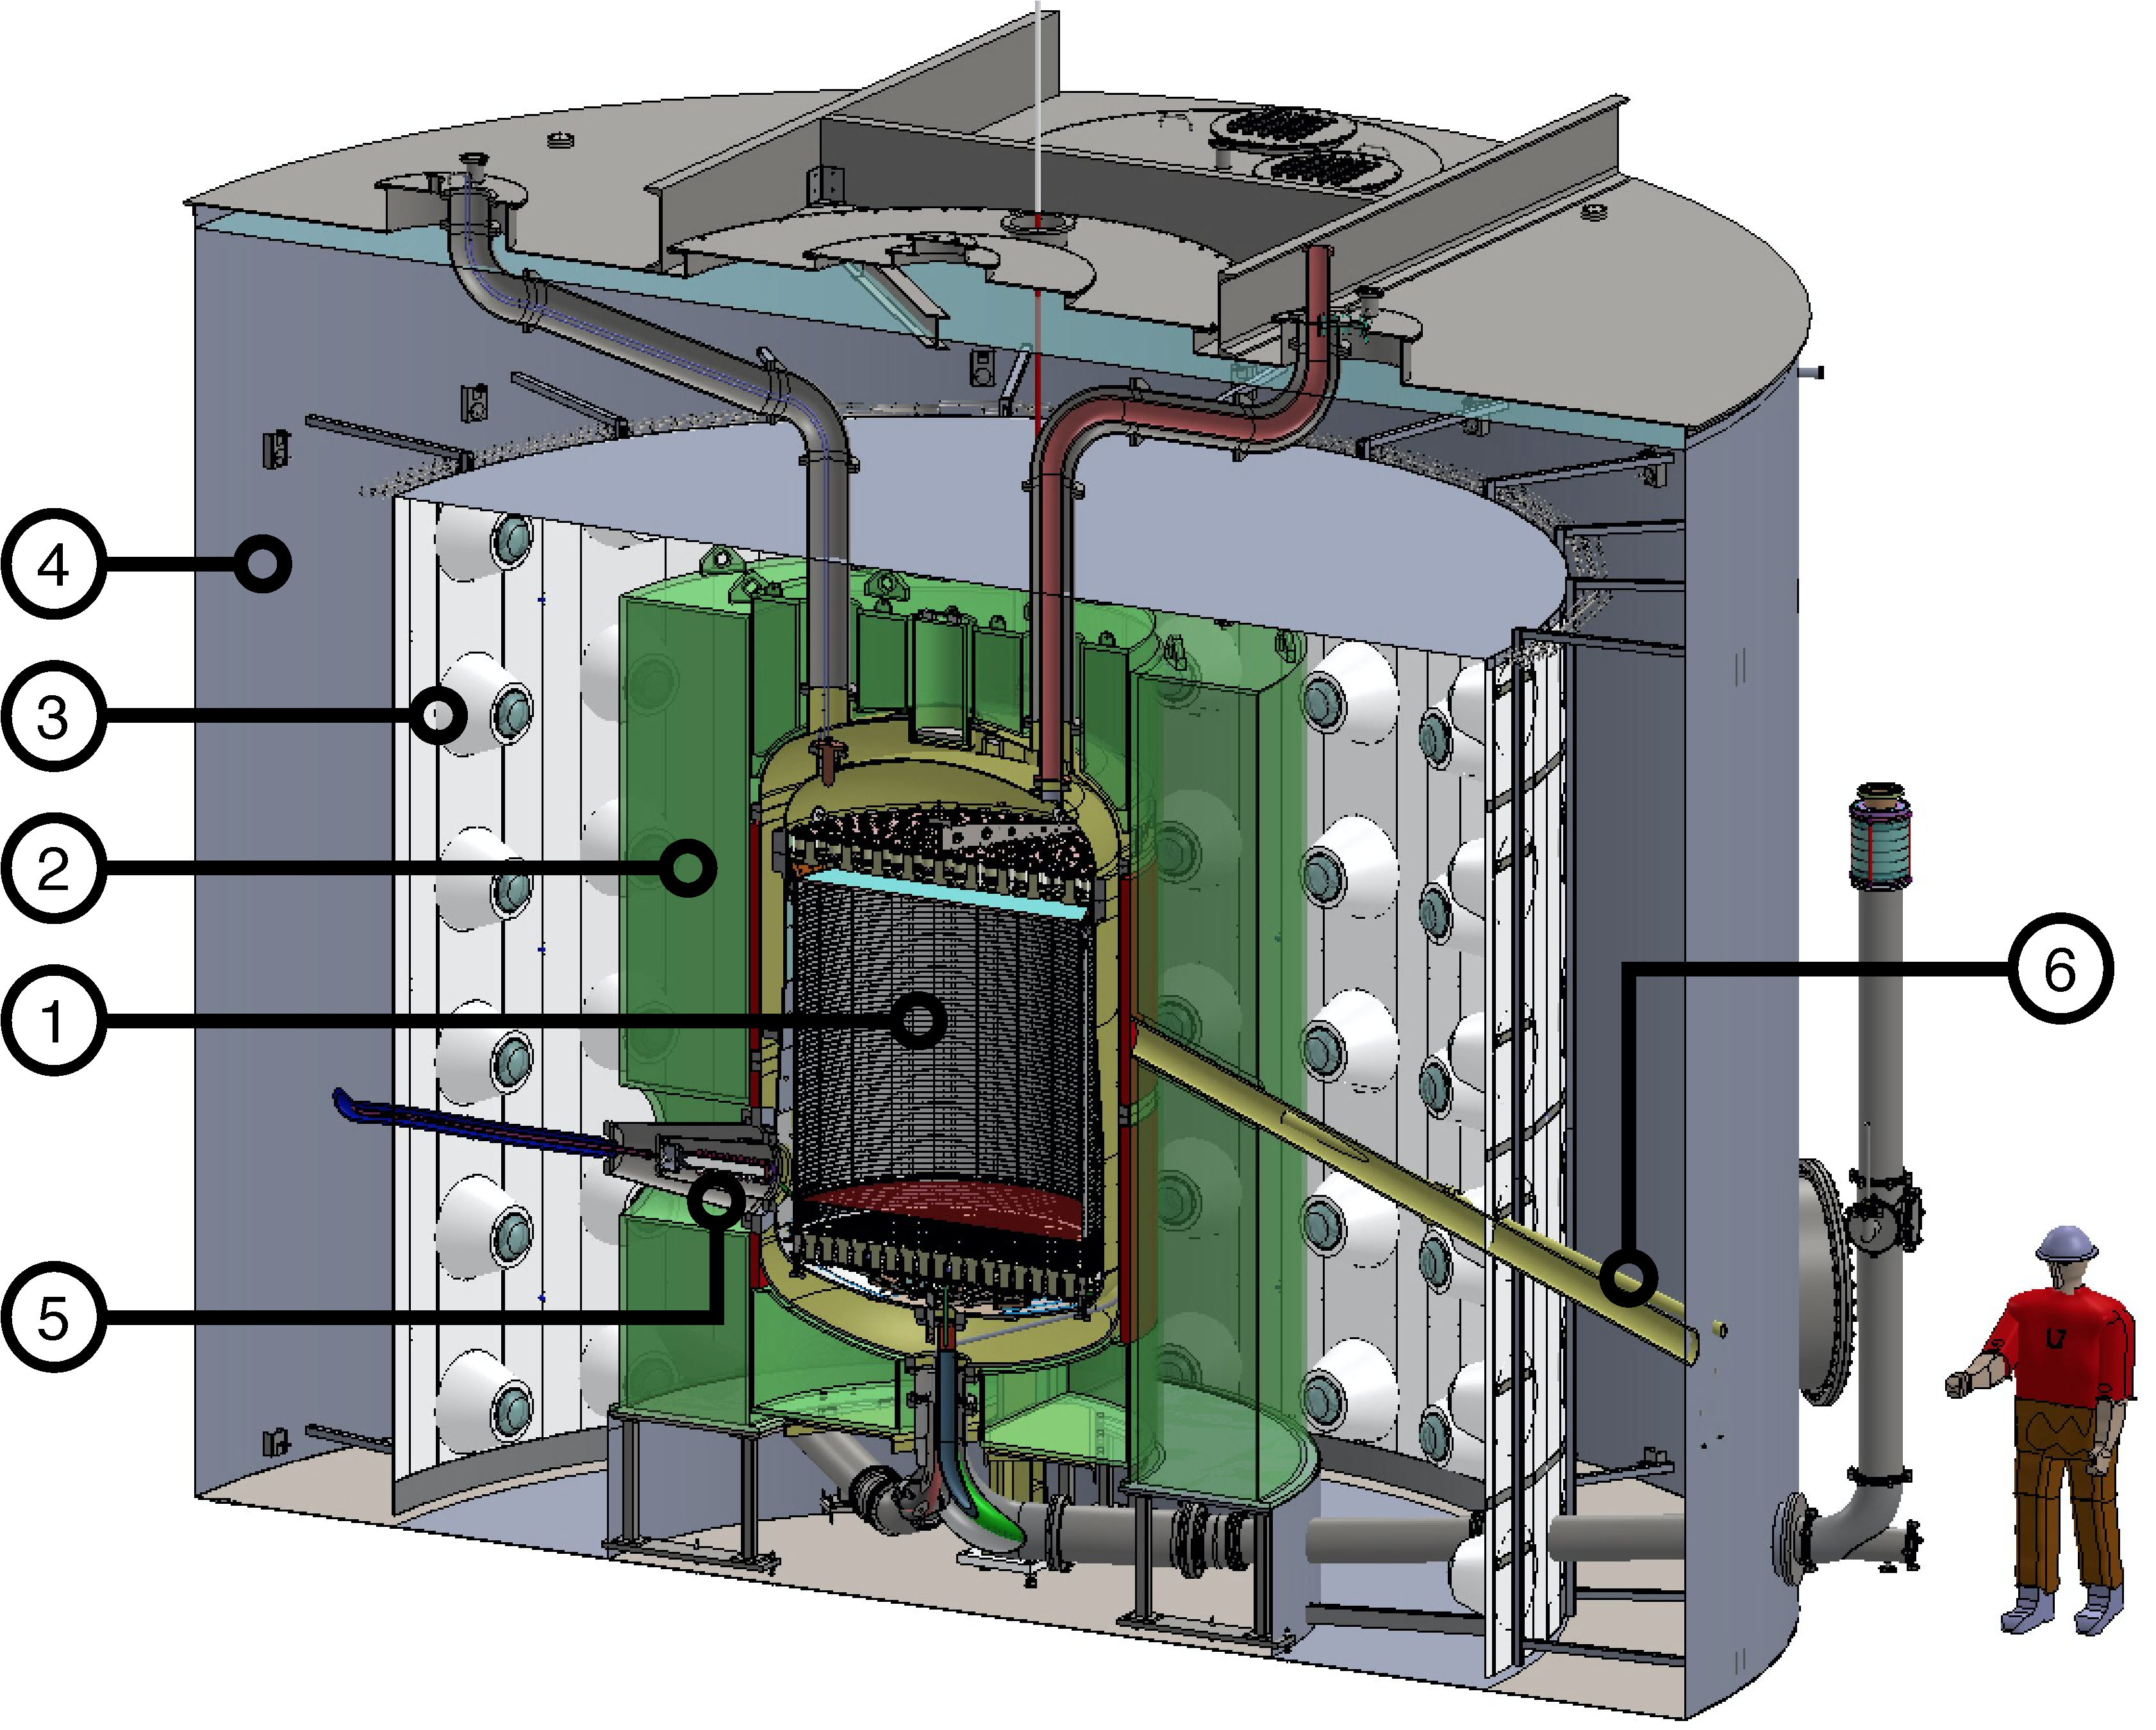
\includegraphics[width=\linewidth]{figures/LZ/LZSchematic.pdf}
    \caption[Schematic of the LZ detector and its the major subsystems.]{Schematic of the LZ detector and its the major subsystems. At the centre is the liquid xenon TPC (1), monitored by two arrays of PMTs and serviced by various cable and LXe conduits (upper and lower). The TPC is contained in a double-walled vacuum insulated titanium cryostat and surrounded on all sides by a GdLS Outer Detector (2). The cathode high voltage connection is made horizontally at the lower left (5). The GdLS is observed by a suite of 8” PMTs (3) standing in the water (4) which provides shielding for the detector. The pitched conduit on the right (6) allows for neutron calibration sources to illuminate the detector \cite{LZNIMA}.}
    \label{fig:LZ/LZDetector}
\end{figure}
\section{Liquid xenon time projection chamber}\label{sec:LZ/LXeTPC}
The LZ TPC holds 7~t (5.6~t fiducial) of LXe above its cathode, there is an additional thin layer (8~mm thick) of gaseous xenon (GXe) at the top of the liquid. The active volume measures approximately 1.5~m in height and diameter and the walls of the TPC are made from PTFE to improve light collection efficiency \cite{LZNIMA}. The TPC, Skin and Xe payload are housed within the Inner Cryostat Vessel (ICV) and the Outer Cryostat Vessel (OCV) provides a vacuum jacket for insulation. Both cryostat vessels are made from low radioactivity titanium \cite{LZ:2017iwn}. When a particle scatters off a LXe atom a prompt scintillation signal (S1) is produced alongside free elections, via ionisation of the LXe atom. The free electrons are drifted to the LXe surface using an applied electric field and are extracted in the GXe layer. As the electrons accelerate through the GXe layer, a proportional amount of scintillation light (S2) is produced. Light produced from these particle interactions is observed by a top and bottom array of 3-inch Hamamatsu R11410–22 PMTs, 494 in total. Using both the S1 and S2 signals, position reconstruction techniques can be used to determine the $xyz$-position of the particle interaction. The time difference between the S1 and S2 signals combined with the drift velocity is used to determine the $z$-position of the interaction whilst the hit pattern of the S2 signal in the top PMT array provides $xy$-position. The operating principle of a TPC can be seen in \autoref{fig:LZ/TPCCartoon}, whilst the main components of the LZ TPC are shown in \autoref{fig:LZ/CAD_TPC}.
\begin{figure}[!ht]
    \centering
    \includesvg[width=\textwidth]{figures/LZ/lz-event.svg}
    \caption{Schematic of a TPC with an event with a S1 and S2 pulse. Each particle interaction with the LXe atoms produces two signals: an initial prompt scintillation (S1) and a second, delayed one from ionisation (S2). The combination of these two signals allows for precise 3D position reconstruction and discrimination between nuclear and electron recoils. Original image courtesy of C. Faham and D. Malling.}
    \label{fig:LZ/TPCCartoon}
\end{figure}

\begin{figure}[!ht]
     \centering
     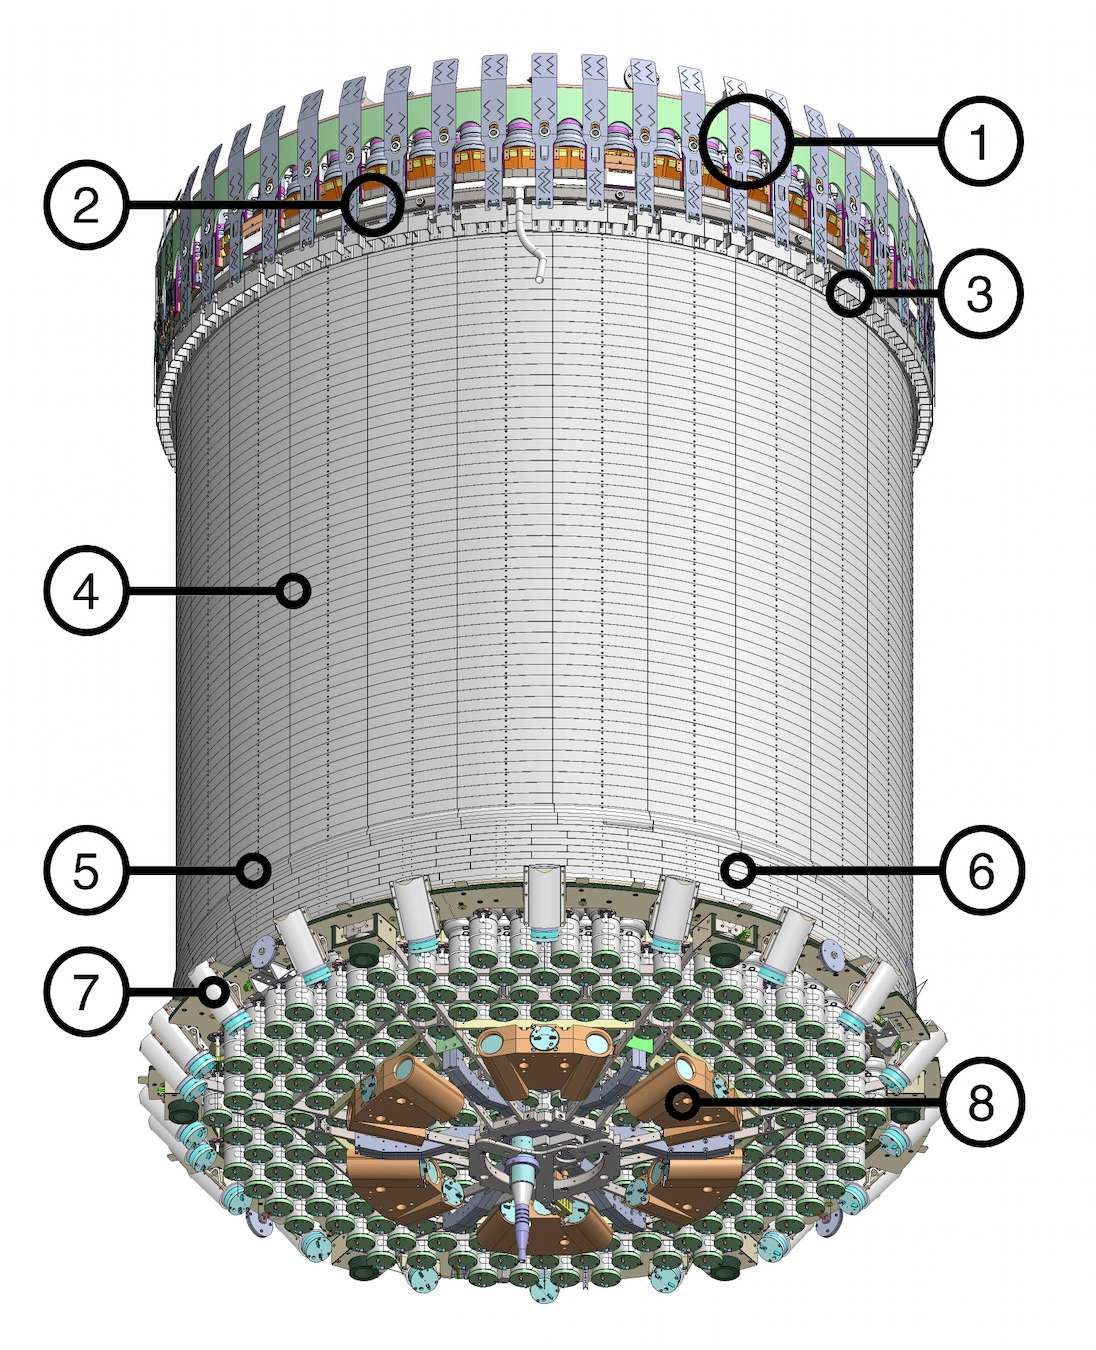
\includegraphics[width=0.5\textwidth]{figures/LZ/CAD_TPC.jpg}
     \caption{Drawing of the TPC \& Skin components: 1-Top PMT array; 2-Gate-anode and weir region (liquid level); 3-Side skin PMTs (1-inch); 4-Field cage; 5-Cathode ring; 6-Reverse field region; 7-Lower side skin PMTs (2-inch); 8-Dome skin PMTs (2-inch) \cite{LZNIMA}.}
     \label{fig:LZ/CAD_TPC}
\end{figure}

\subsection{Particle-Xenon interactions within a TPC}\label{sec:LZ/XeInteractionsTPC}
As a particle traverses the LXe volume it can interact with either the atomic nucleus, producing a nuclear recoil (NR), or with the surrounding electron cloud, producing an electronic recoil (ER). Both processes result in the pair of signals discussed in \autoref{sec:LZ/LXeTPC}. The S1 signal is produced via the following mechanism. The excited Xe atom, Xe$^{*}$, combines with a nearby ground state Xe atom to form an excimer state, Xe$_{2}^{*\nu}$, which is both an electronically and vibrationally excited molecule. Through collisions with other Xe atoms, energy in the vibrational modes of the excimer is lost. The excited pair de-excite further as the electronic excitation energy is released as a pair of vacuum-ultraviolet (VUV), at a mean wavelength of 178~nm \cite{Schumann:2014uva}.
The Xe atom also undergoes ionisation due to the displacement of the nucleus during the collision releasing electrons. A positively charged Xe$^{+}$ ion combines with a neutral Xe atom to form a positively charged dimer Xe$^{+}_{2}$. Most of the electrons that are emitted in the ionisation are drifted away from the collision site by the applied electric field. However some of the ionised electrons produced in the cascade recombine with the molecule prior to it splitting to form a highly excited Xe atom. A final series of relaxation occurs in a similar manner to the excitation luminescence excimer. A schematic which describes the process of producing the S1 and S2 signal can be seen in \autoref{fig:LZ/XenonSigalProduction}.
\begin{figure}[!ht]
    \centering
    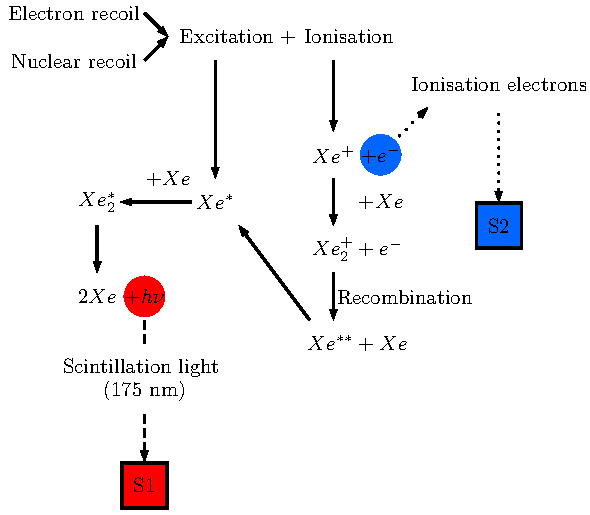
\includegraphics[width=0.8\linewidth]{figures/LZ/Xenon_interaction.pdf}
    \caption{A schematic of the signal production and collection in a dual phase xenon time projection chamber.}
    \label{fig:LZ/XenonSigalProduction}
\end{figure}
To understand what particle has passed through the LXe it is important to determine the energy deposited in interaction with the Xe atom. This can be described using the following equation:
\begin{equation}
    E=\frac{W}{L}(n_{ex}+n_{i})
    \label{eqn:EnergyRec_noG}
\end{equation}
Where $W$ is the average energy required to produced either one scintillation photon or ionisation electron, which has been measured to be $13.7\pm0.4$~eV \cite{Goetzke:2016lfg, Dahl:2009nta}.
$L$ is referred to as the "Lindhard factor" or "quenching" accounting for the reduction of produced light and charge as energy is lost to heat. For electron recoils $L$ is taken as unity, this implies that the heat-loss is constant with energy allowing it to be absorbed into the value of $W$ \cite{Rischbieter:2022}. The Lindhard factor for nuclear recoils is observed to be a function of deposited energy as the interaction energy is not linearly related to the observed total quanta \cite{Sorensen:2011bd}.
$n_{ex}$ and $n_{i}$ represent the number of excited atoms and ionised atoms respectively and are proportional to pulse area of the S1 and S2 pulses observed in the TPC respectively. The constants of proportionality are $g_1$ and $g_2$ and represent the S1 light collection efficiency and the electron extraction efficiency of the detector respectively. Thus \autoref{eqn:EnergyRec_G} can be modified to describe the energy deposition using:
\begin{equation}
    E=\frac{W}{L}\bigg(\frac{S1}{g_1}+\frac{S2}{g_2}\biggl)
    \label{eqn:EnergyRec_G}
\end{equation}

\subsection{NR and ER discrimination}\label{LZ/NRERDiscrim}
The ratio of of light to charge produced differs between NRs and ERs. This can be directly observed through the S1 and S2 pulse areas produced from the interactions, particularly the ratio, $\text{log}_{10}(\text{S2})/\text{S1}$. This method demonstrates 95\% discrimination against ER with a 50\% NR acceptance \cite{lzSens}. This is key in the search for WIMPs where we would expect to observe an NR when a WIMP passes through the TPC. However, the dominant backgrounds such as $\beta$-decays from Rn daughter isotopes and \textsuperscript{85}Kr and $\gamma$ radiation from detector components all produce ER events in the LXe. Both ER and NR events form distinctive band structure in $\text{log}_{10}(\text{S2})/\text{S1}$ space, as shown in \autoref{fig:LZ/NRERBandExample}, where the width of the bands is due to electron-ion recombination at the interaction site whilst the overall separation is due to the ratio of ionisation to excitation in the interaction \cite{Dahl:2009nta}.

\begin{figure}[!ht]
    \centering
    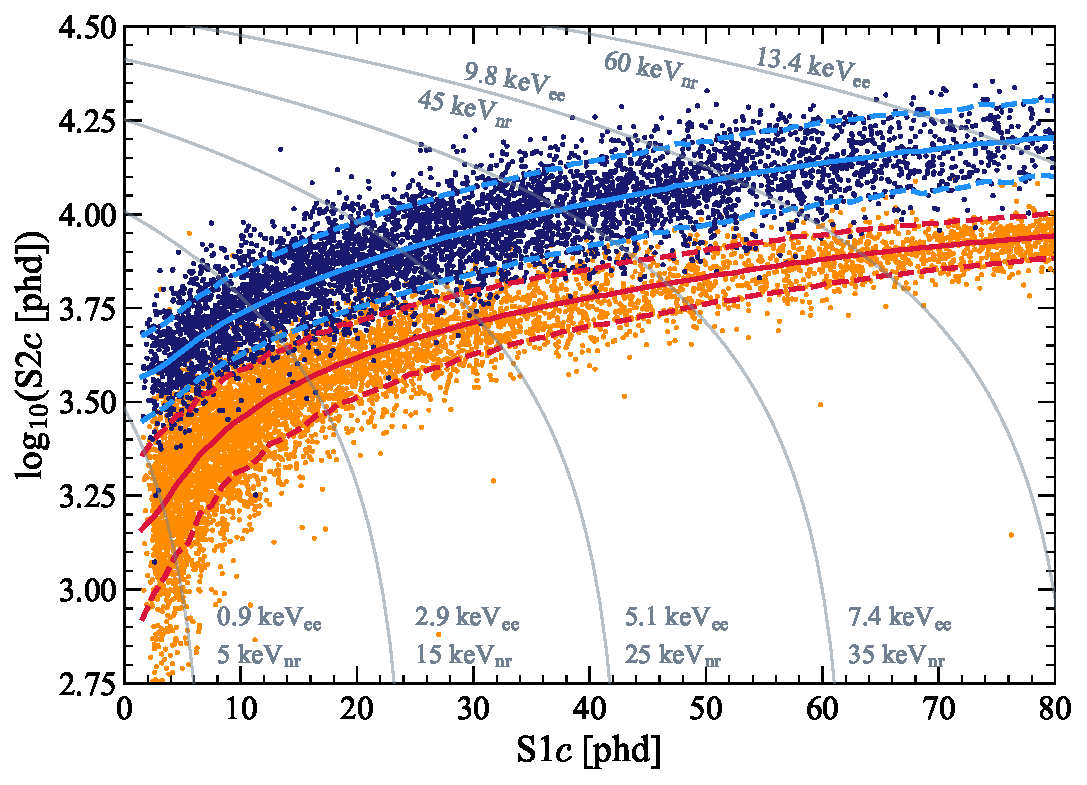
\includegraphics[width=0.8\linewidth]{figures/LZ/SR1WS_calOnly_0629.pdf}
    \caption[Discrimination between ER and NR in LZ using calibration events.]{Discrimination between ER and NR in LZ using calibration events in $\text{log}_{10}\text{S2}_{\text{c}}/\text{S1}_{\text{c}}$ for the tritium source (dark blue points, 5343 events) and the DD neutron generator (orange points, 6324 events). Solid blue (red) lines indicate the median of the ER (NR) simulated distributions, and the dotted lines indicate the 10\% and 90\% quantiles. The thin gray lines represent contours of constant electron-equivalent energy (keV$_{\text{ee}}$) and nuclear recoil energy (keV$_{\text{nr}}$) \cite{LZ:2022lsv}.}
    \label{fig:LZ/NRERBandExample}
\end{figure}

\section{Xenon Skin}\label{sec:LZ/Skin}
The TPC is surrounded by a layer of LXe, the region contains around 2~t of LXe between the field cage and the inner cryostat vessel \cite{LZNIMA}. The primary motivation for including this layer of LXe was to provide dielectric insulation between the two elements. Unlike XENONnT, LZ's main competitor, this region is instrumented for optical readout acting as a scintillation-only veto detector for gamma ray interactions in the TPC~\cite{XENON:2024wpa}. The region is known as the "Skin" and can be divided into two regions: Barrel and Dome. The Barrel contains 93 1-inch Hamamatsu R5820 PMTs at the top of the Barrel looking down and 38 2-inch Hamamatsu R8778 PMTs; 20 at the bottom of the Barrel looking up, and 18 in the Dome region below the TPC \cite{LZNIMA}. The layout of the Skin PMTs with respect to the TPC can be seen in \autoref{fig:LZ/CAD_TPC}.

\section{Outer Detector}\label{sec:LZ/LZOD}
It has been shown in previous sections that dual phase TPC has the capability to distinguish between ER and NR interactions in the LXe, however it does not have the capability to determine what particle caused the recoil. Neutrons are the primary source of NRs as they scatter of the Xe nuclei and mimic a signal similar to a WIMP. Neutrons are likely to scatter multiple times in the TPC or the OD whereas WIMPs would scatter only once in the TPC due to differences in their respective interactions cross sections. LZ is taking advantage of this principle by surrounding the TPC with a neutron detector to increases the discrimination against NR backgrounds. This detector is the Outer Detector.
%and together with the Xe Skin comprises the LZ Veto System. 
The outer cryostat housing the TPC is surrounded near hermetically by ten acrylic vessels filled with  Gadolinium loaded liquid scintillator (GdLS). The GdLS is observed by 120 PMTs and surrounded by 238~t of DI water which provides additional shielding to the detector and can be used to detect muons which emit Cherenkov radiation as they pass through the water. An exploded view of these vessels can be seen in \autoref{fig:LZ/ODTanks}.
\begin{figure}[!ht]
    \centering
    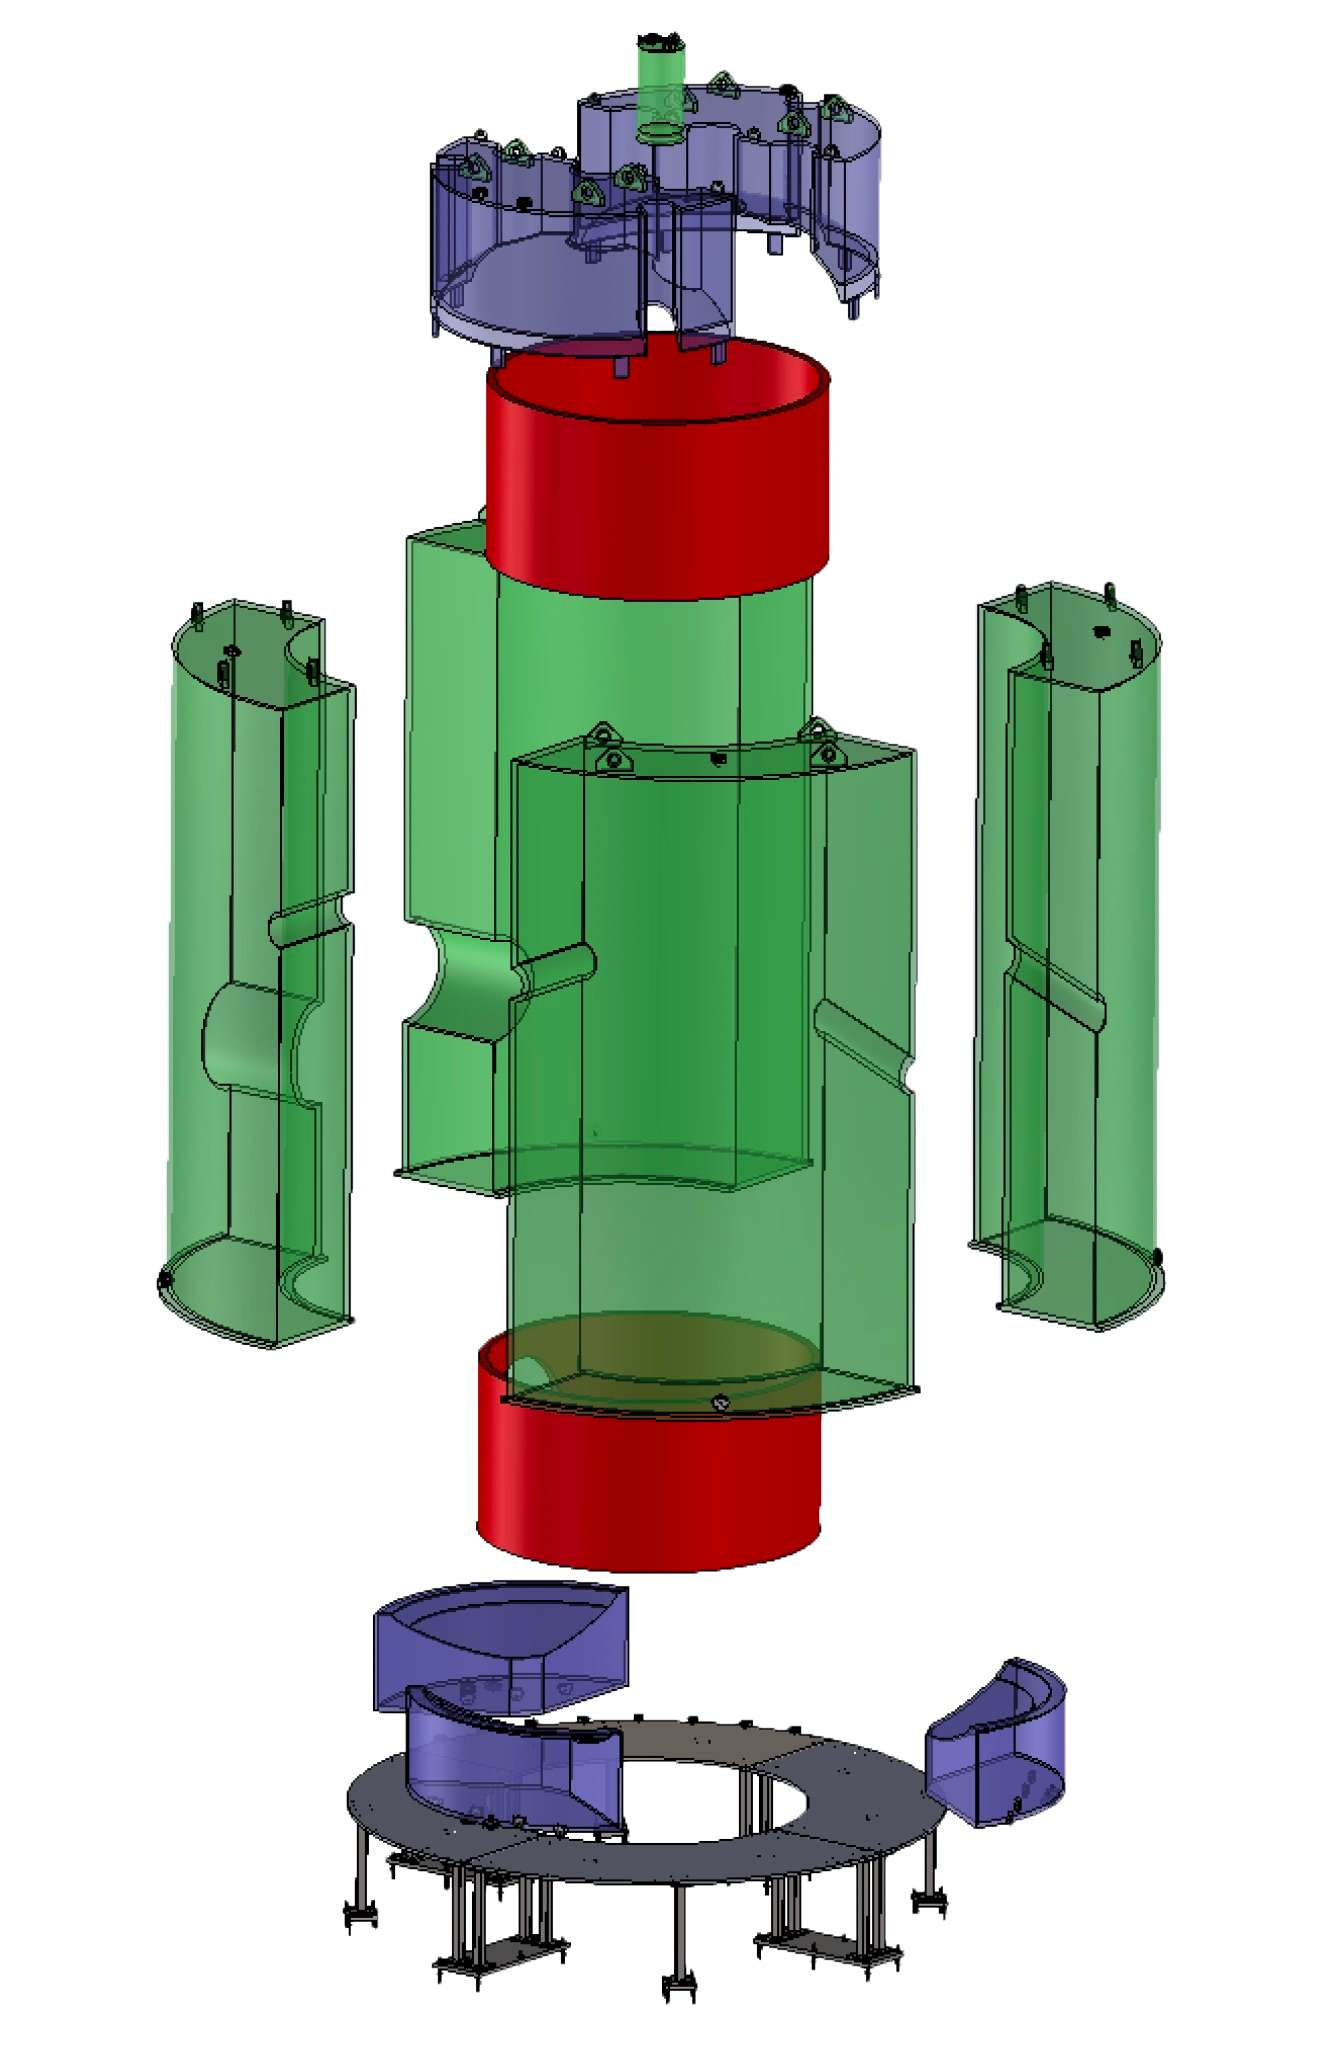
\includegraphics[width=0.5\linewidth]{figures/LZ/CAD_ODTanks.jpg}
    \caption{The Outer Detector vessels in an exploded view. The four large side vessels (SATs) are shown in green, the five small vessels (two top (TATs) and three bottom (BATs)) are shown in blue. The stainless steel base is given in grey and the foam water displacers in red. There is an additional small vessel shown in green at the top which is removed for photo-neutron calibration source deployment \cite{LZNIMA}.}
    \label{fig:LZ/ODTanks}
\end{figure}

\subsection{Liquid scintillator}\label{sec:LZ/LS}
The primary detection medium for the OD is the GdLS, chosen for its excellent efficiency for neutrons and gammas that reach the OD \cite{LZTDR}. The composition of the GdLS mixture is shown in \autoref{tab:LZ/GdLSComp}. The base of the LS mixture is Linear-alkylbenzene (LAB), which acts as a solvent for the other components of the mixture. In addition to the LAB, the fluor 2,5-diphenyloxazole (PPO), and the wavelength shifter 1,4-bis(2-methylstyryl(benzene)) (Bis-MSB) are considered as the LS. As particles pass through the LS, the LAB component is excited as the particles deposit energy along the tracks. Through a series of chemical reactions, the excited LAB transmits energy to the fluor. As the excited fluor de-excites, it emits light with wavelengths up to 380~nm. Due to the short absorption lengths of the LS below 380~nm (approximately 1~m), Bis-MSB is included as a wavelength shifter. The Bis-MSB absorbs the photons produced by the fluor and emits photons with wavelengths between 410~nm~-~425~nm with absorption lengths over 10~m. Bis-MSB is a crucial component of the mixture as wavelengths of the emitted photons overlap with the PMT sensitivity spectrum and absorption lengths satisfy the detector geometry.
The mixture is additionally loaded with Gd with a mass fraction of 0.1\%. Gd has a very high $(n,\gamma)$ cross-section so improves both the efficiency and intensity of the neutron capture signal \cite{LZTDR}. Due to the effectiveness of the Gd, only a small mass fraction is needed to dominate over neutron capture on protons in the LS. To dissolve the Gd in solution with the LS it is bound to a chelating agent, 3,5,5-trimethylhexanoic acid (TMHA) in a 3:1 ratio \cite{LZTDR,Haselschwardt:2018vmp}.
\begin{table}[!ht]
    \centering
    \caption{Chemical components in 1L of GdLS, adapted from Ref.~\cite{Haselschwardt:2018vmp}.}
    \begin{tabular}{llll}
        \hline\hline
        \textbf{Component} & \textbf{Molecular Formula} & \textbf{Mass [g/L]} & \textbf{Mass Fraction} \\
        \hline
        LAB & $\text{C}_{17.14}\text{H}_{28.28}$ & 853.55 & 99.25\\
        PPO & $\text{C}_{15}\text{H}_{11}\text{NO}$ & 3.00 & 0.35 \\
        bis-MSB & $\text{C}_{24}\text{H}_{22}$ & 0.01 & 0.0011\\
        TMHA & $\text{C}_{9}\text{H}_{17}\text{O}_{2}^{-}$ & 2.58 & 0.003\\
        Gd & Gd & 0.86 & 0.1 \\
        \hline
        GdLS & $\text{C}_{17.072} \text{H}_{28.128} \text{O}_{0.0126} \text{N}_{0.0037} \text{Gd}_{0.0015}$ & 860.00 & 100 \\
        \hline\hline
    \end{tabular}
    \label{tab:LZ/GdLSComp}
\end{table}
\subsubsection{Neutron capture in the OD}\label{sec:LZ/NeutronCapture}
As previously mentioned, Gadolinium has the largest capture cross-section for thermal neutrons of any known stable elements: 49~kb \cite{Hagiwara:2018kmr}. This is due to contributions of two isotopes $^{155}\text{Gd}$ (61~kb) and especially $^{157}\text{Gd}$ (254~kb) \cite{Hagiwara:2018kmr}. After a thermal neutron captures on $^{157}\text{Gd}$, the $^{158}\text{Gd}^*$ compound nucleus remains in a 7837 keV excited state, a subsequent de-excitation occurs via a cascade of on average 4-5 $\gamma$-ray emissions \cite{Hagiwara:2018kmr}. The de-excitation is illustrated in \autoref{fig:LZ/Gd158Deexcite}. The continuum component of the $\gamma$-ray spectrum see in \autoref{fig:LZ/ODEnergySpec} is depicted in \autoref{fig:LZ/Gd158Deexcite} where the multi-step de-excitations of $^{158}\text{Gd}^*$ can occur between unresolvable levels in quasicontinuum (dashed lines), within discrete levels (solid lines). This results in a random distribution of both the number and energy of the emitted $\gamma$-rays. 

\begin{figure}[!ht]
    \centering
    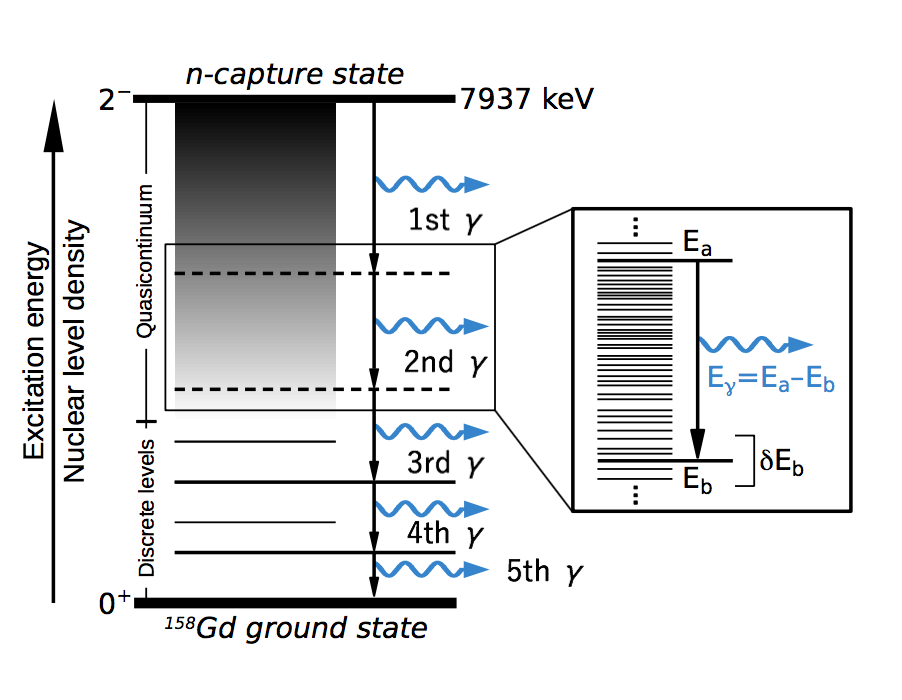
\includegraphics[width=0.8\linewidth]{figures/LZ/ContinuumEmission2.png}
    \caption{Illustration of the multi-step $\gamma$-ray emission of an excited $^{158}\text{Gd}^*$ following the thermal $^{157}\text{Gd}(n,\gamma)$ reaction. The de-excitation to the ground state can occur via many intermediate levels. Adapted from Ref.~\cite{Hagiwara:2018kmr}.}
    \label{fig:LZ/Gd158Deexcite}
\end{figure}
In addition to neutron capture of Gd, hydrogen also produces a neutron capture signal. Hydrogen has thermal neutron capture cross section of 0.33~b which appears meagre in comparison with Gd, however due to the abundance of hydrogen in the LS, acrylic, and water, a significant number of neutron captures are observed. Following the capture of a thermal neutron, the excited deuterium atom decays to its ground state and emits a single 2.2~MeV $\gamma$-ray \cite{LZTDR}. The prominent peak resulting from the hydrogen capture can be seen in the OD energy spectrum shown in \autoref{fig:LZ/ODEnergySpec}.
\begin{figure}[!ht]
    \centering
    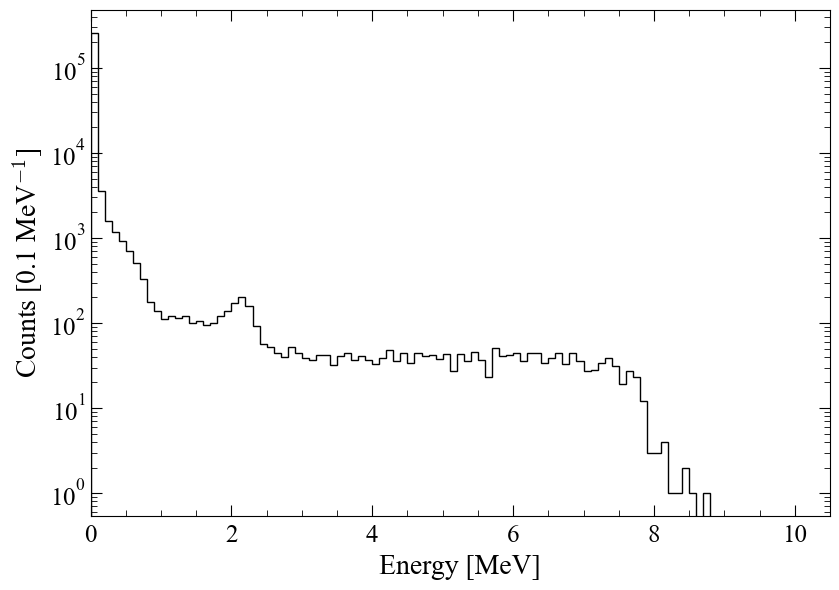
\includegraphics[width=0.8\linewidth]{figures/LZ/ODEnergySpec.png}
    \caption{AmLi energy spectrum measured with LZ Outer Detector with coincident single scatter signals in the TPC, here simple data quality cuts have been applied. The distinctive hydrogen capture peak can be seen at 2.2~MeV, whilst the continuous $\gamma$-ray spectrum from the Gd Capture has the expected end point at $\mathtt{\sim}$8~MeV.}
    \label{fig:LZ/ODEnergySpec}
\end{figure}
By doping LS with Gd, the efficiency for detecting at least one of the capture gammas is very high compared to having pure LS. Another advantage of Gd-doping is reduction in the time delay for neutron capture from 220~\textmu s to 28~\textmu s intern reducing the length of the window needed for vetoing by a factor of 7 \cite{LZTDR}. Detailed simulations by the LZ Collaboration initially expected to use a veto window of 125~\textmu s, however it was found that neutrons also captured in the acrylic up to 10\% of the time \cite{LZTDR}. Further studies by the author also found that neutrons captured in the water which had partially saturated foam displacer between the acrylic tanks and OCV. This effect further extended the required veto window to 600~\textmu s. This study is discussed further in \autoref{sec:VetoEff/NCT}.

\subsection{PMT system}\label{sec:LZ/ODPMTs}
Interactions in the GdLS and water are monitored by 120 Hamamatsu 8-inch R5912 photo-multiplier tubes (PMTs) arranged as shown in \autoref{fig:LZ/ODPMT_Array}. 
This model of PMT has been used successfully prior to their use in LZ at Daya Bay whose detector design is echoed in the LZ OD design \cite{Cao:2016vwh}. The R5912 PMTs were chosen because of the following reasons:
\begin{enumerate} 
    \item The spectral response ranges from 300~nm to 650~nm, with a peak wavelength at 420~nm. This encompasses the range of the scintillation light from the LAB mix between 390~nm to 440~nm \cite{Haselschwardt:2018vmp}. The comparison can be made comparing the plots in \autoref{fig:LZ/ODPMTSpecRes}.
    \item The quantum efficiency covers the relevant range, with an average expected value of $\sim25\%$ at 430~nm, as shown in \autoref{fig:LZ/ODPMTQE}.
    \item The radioactivity levels of the PMTs and support structure is a fairly weak constraint due to the 84~cm of water separating them from any active volume. In the scintillator itself, the simulated event rate from the PMT radioactivity is $<4~\text{Hz}$ \cite{LZTDR}. 
\end{enumerate}
\begin{figure}[!ht]
    \centering
    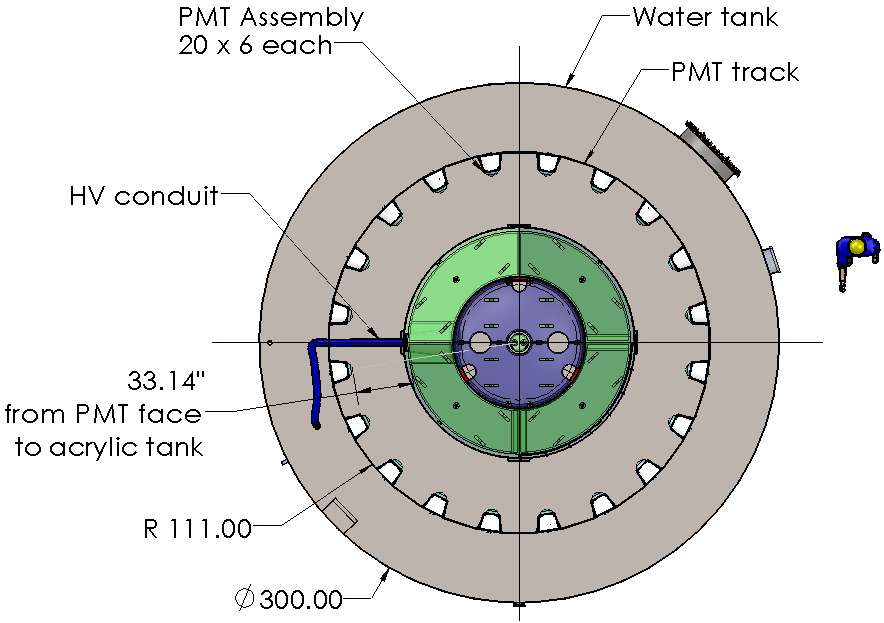
\includegraphics[width=0.7\linewidth]{figures/LZ/OD_PMT_support.jpg}
    \caption{Plan view of the OD PMT support system. The 20 PMT ladders are mounted to a circular track attached to the walls of the water tank \cite{LZTDR}.}
    \label{fig:LZ/ODPMT_Array}
\end{figure}
\begin{figure}[!ht]
     \centering
     \begin{subfigure}{0.47\textwidth}
         \centering
         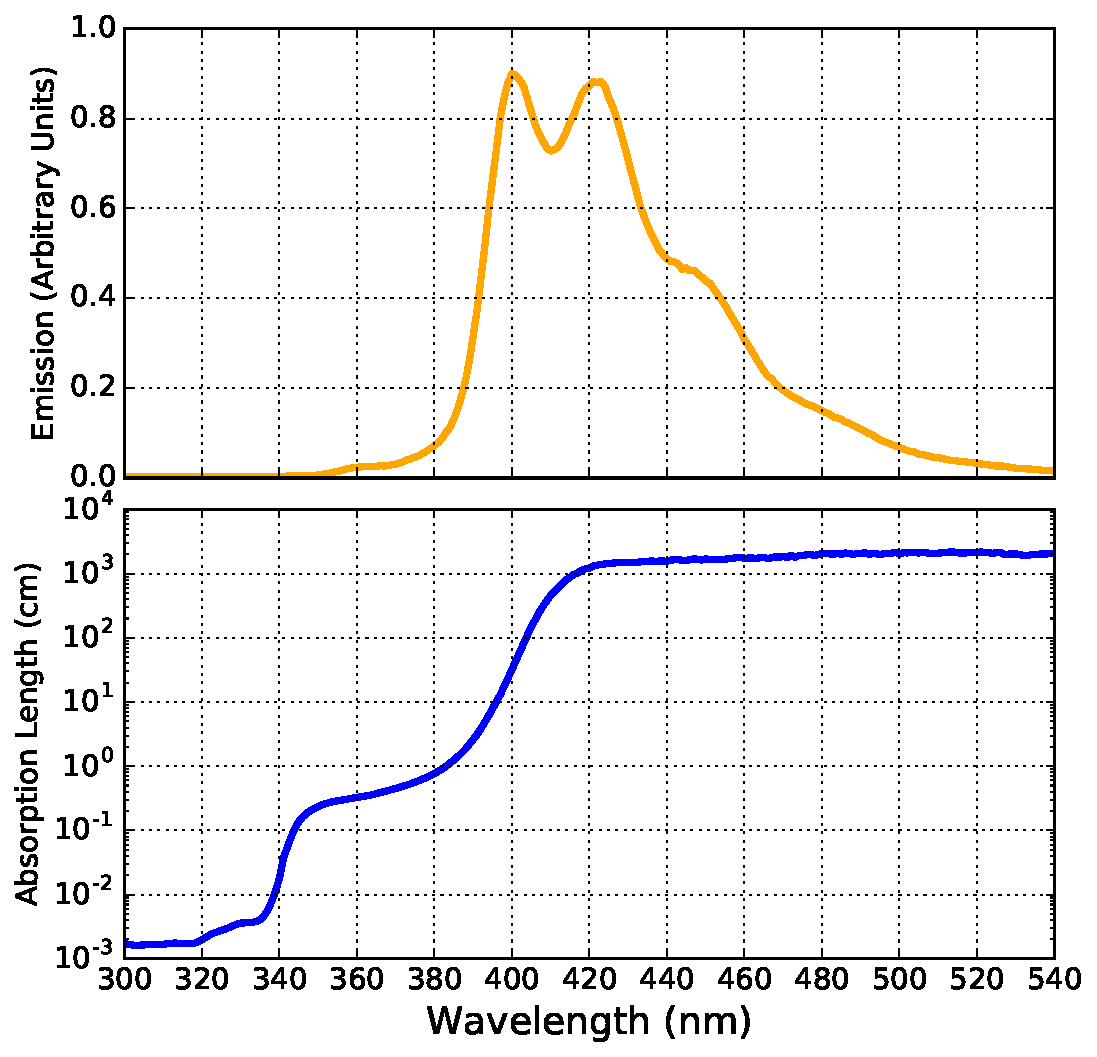
\includegraphics[width=\textwidth]{figures/LZ/GdLS_SpectralResponse.pdf}
         \caption{Wavelength dependence of two optical properties of the GdLS. \textbf{Top:} Emission spectrum of scintillation light. \textbf{Bottom:} The  absorption length of GdLS \cite{Haselschwardt:2018vmp}.}
         \label{fig:LZ/GdLSSpecRes}
     \end{subfigure}
     \hfill
     \begin{subfigure}{0.47\textwidth}
         \centering
         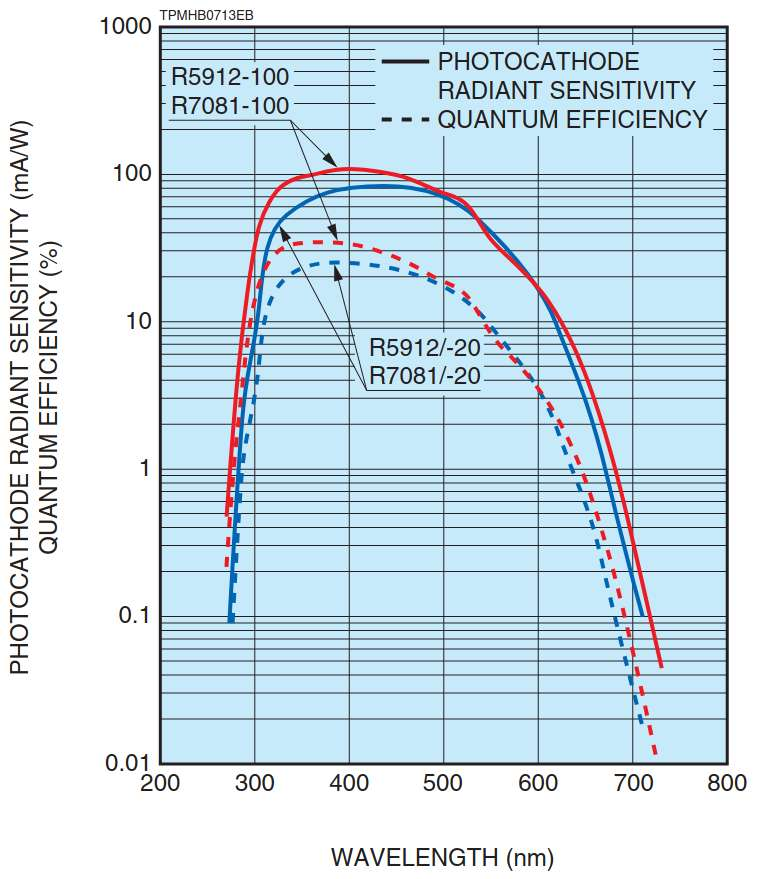
\includegraphics[width=\textwidth]{figures/LZ/ODPMT_QEvsWL.png}
         \caption{Wave length dependence of the quantum efficiency of the Hamamatsu 8-inch R5912 photo-multiplier tube. Adapted from Ref.~\cite{HamamatsuR5912}}
         \label{fig:LZ/ODPMTQE}
     \end{subfigure}
     \caption{A comparison of the wavelength dependence of key optical parameters for both the GdLS and PMTs.}
     \label{fig:LZ/ODPMTSpecRes}
\end{figure}
Prior to the installation of the PMTs at SURF, rigorous testing to fully characterise the response of tubes was carried out by groups from Brandeis University and the IBS Center for Underground Physics. Further details of the quality assurance testing is documented in Ref.~\cite{lkorley:thesis}.

\subsection{Outer detector optical calibration system}\label{sec:LZ/ODOCS}
LZ uses an optical calibration system to monitor: the PMT gain/single photoelectron (SPhE) size; afterpulsing rates; and the optical properties of the acrylic and scintillator. Light produced by the LED-driven system is injected into the OD at 35 different locations. Thirty injection points are evenly distributed throughout the PMT array  (10 azimuthal positions at 3 heights as shown in \autoref{fig:LZ/OCSPositions}). Four of the injection points are each positioned in centre of the side acrylic tanks facing upwards to monitor the optical properties of the GdLS. One final injection points is positioned in the outer rim of a side acrylic tank also facing upwards and is used to monitoring the optical properties of the acrylic.
\begin{figure}[!ht]
    \centering
    \includegraphics[width=\linewidth]{figures/LZ/OD_PMT_CAD_picture_v4.png}
    \caption{\textbf{Left:} A cross-section of a CAD drawing of the OD. The three  heights of the 10 azimuthal positions of the optical fibre injection points are labelled 1-3. Two injection positions under the side acrylic tanks which point upwards are labelled 4 and 5. \textbf{Right:} A photograph of the OD PMT array showing the point of an injection point relatively to the surrounding PMTs.}
    \label{fig:LZ/OCSPositions}
\end{figure}
Duplex fibres are used to inject light pulses produced by LEDs to the different locations. For the thirty injection points situated within the PMT, 435~nm LEDs are used to match the peak wavelength and quantum efficiency of OD PMTs. Only one core in the fibre is used, the additional core is a backup in the event of any damage to the first core. 435~nm and 450~nm were doing for the injection points facing into the LS to monitor optical degradation of the scintillator. Below 420~nm the absorption length of GdLS decreases significantly as shown in \autoref{fig:LZ/GdLSSpecRes}, if the scintillator degrades this region shifts to higher wavelengths. A similar approach is taken for monitoring the optical properties of the acrylic using 390~nm and 435~nm LEDs. The transmission of light through the acrylic varies with wavelength, as shown in \autoref{fig:LZ/AcrylicQA}. Monitoring the optical properties of the acrylic and scintillator during science runs is key to ensure consistent light collection during science runs.
\begin{figure}[!ht]
    \centering
    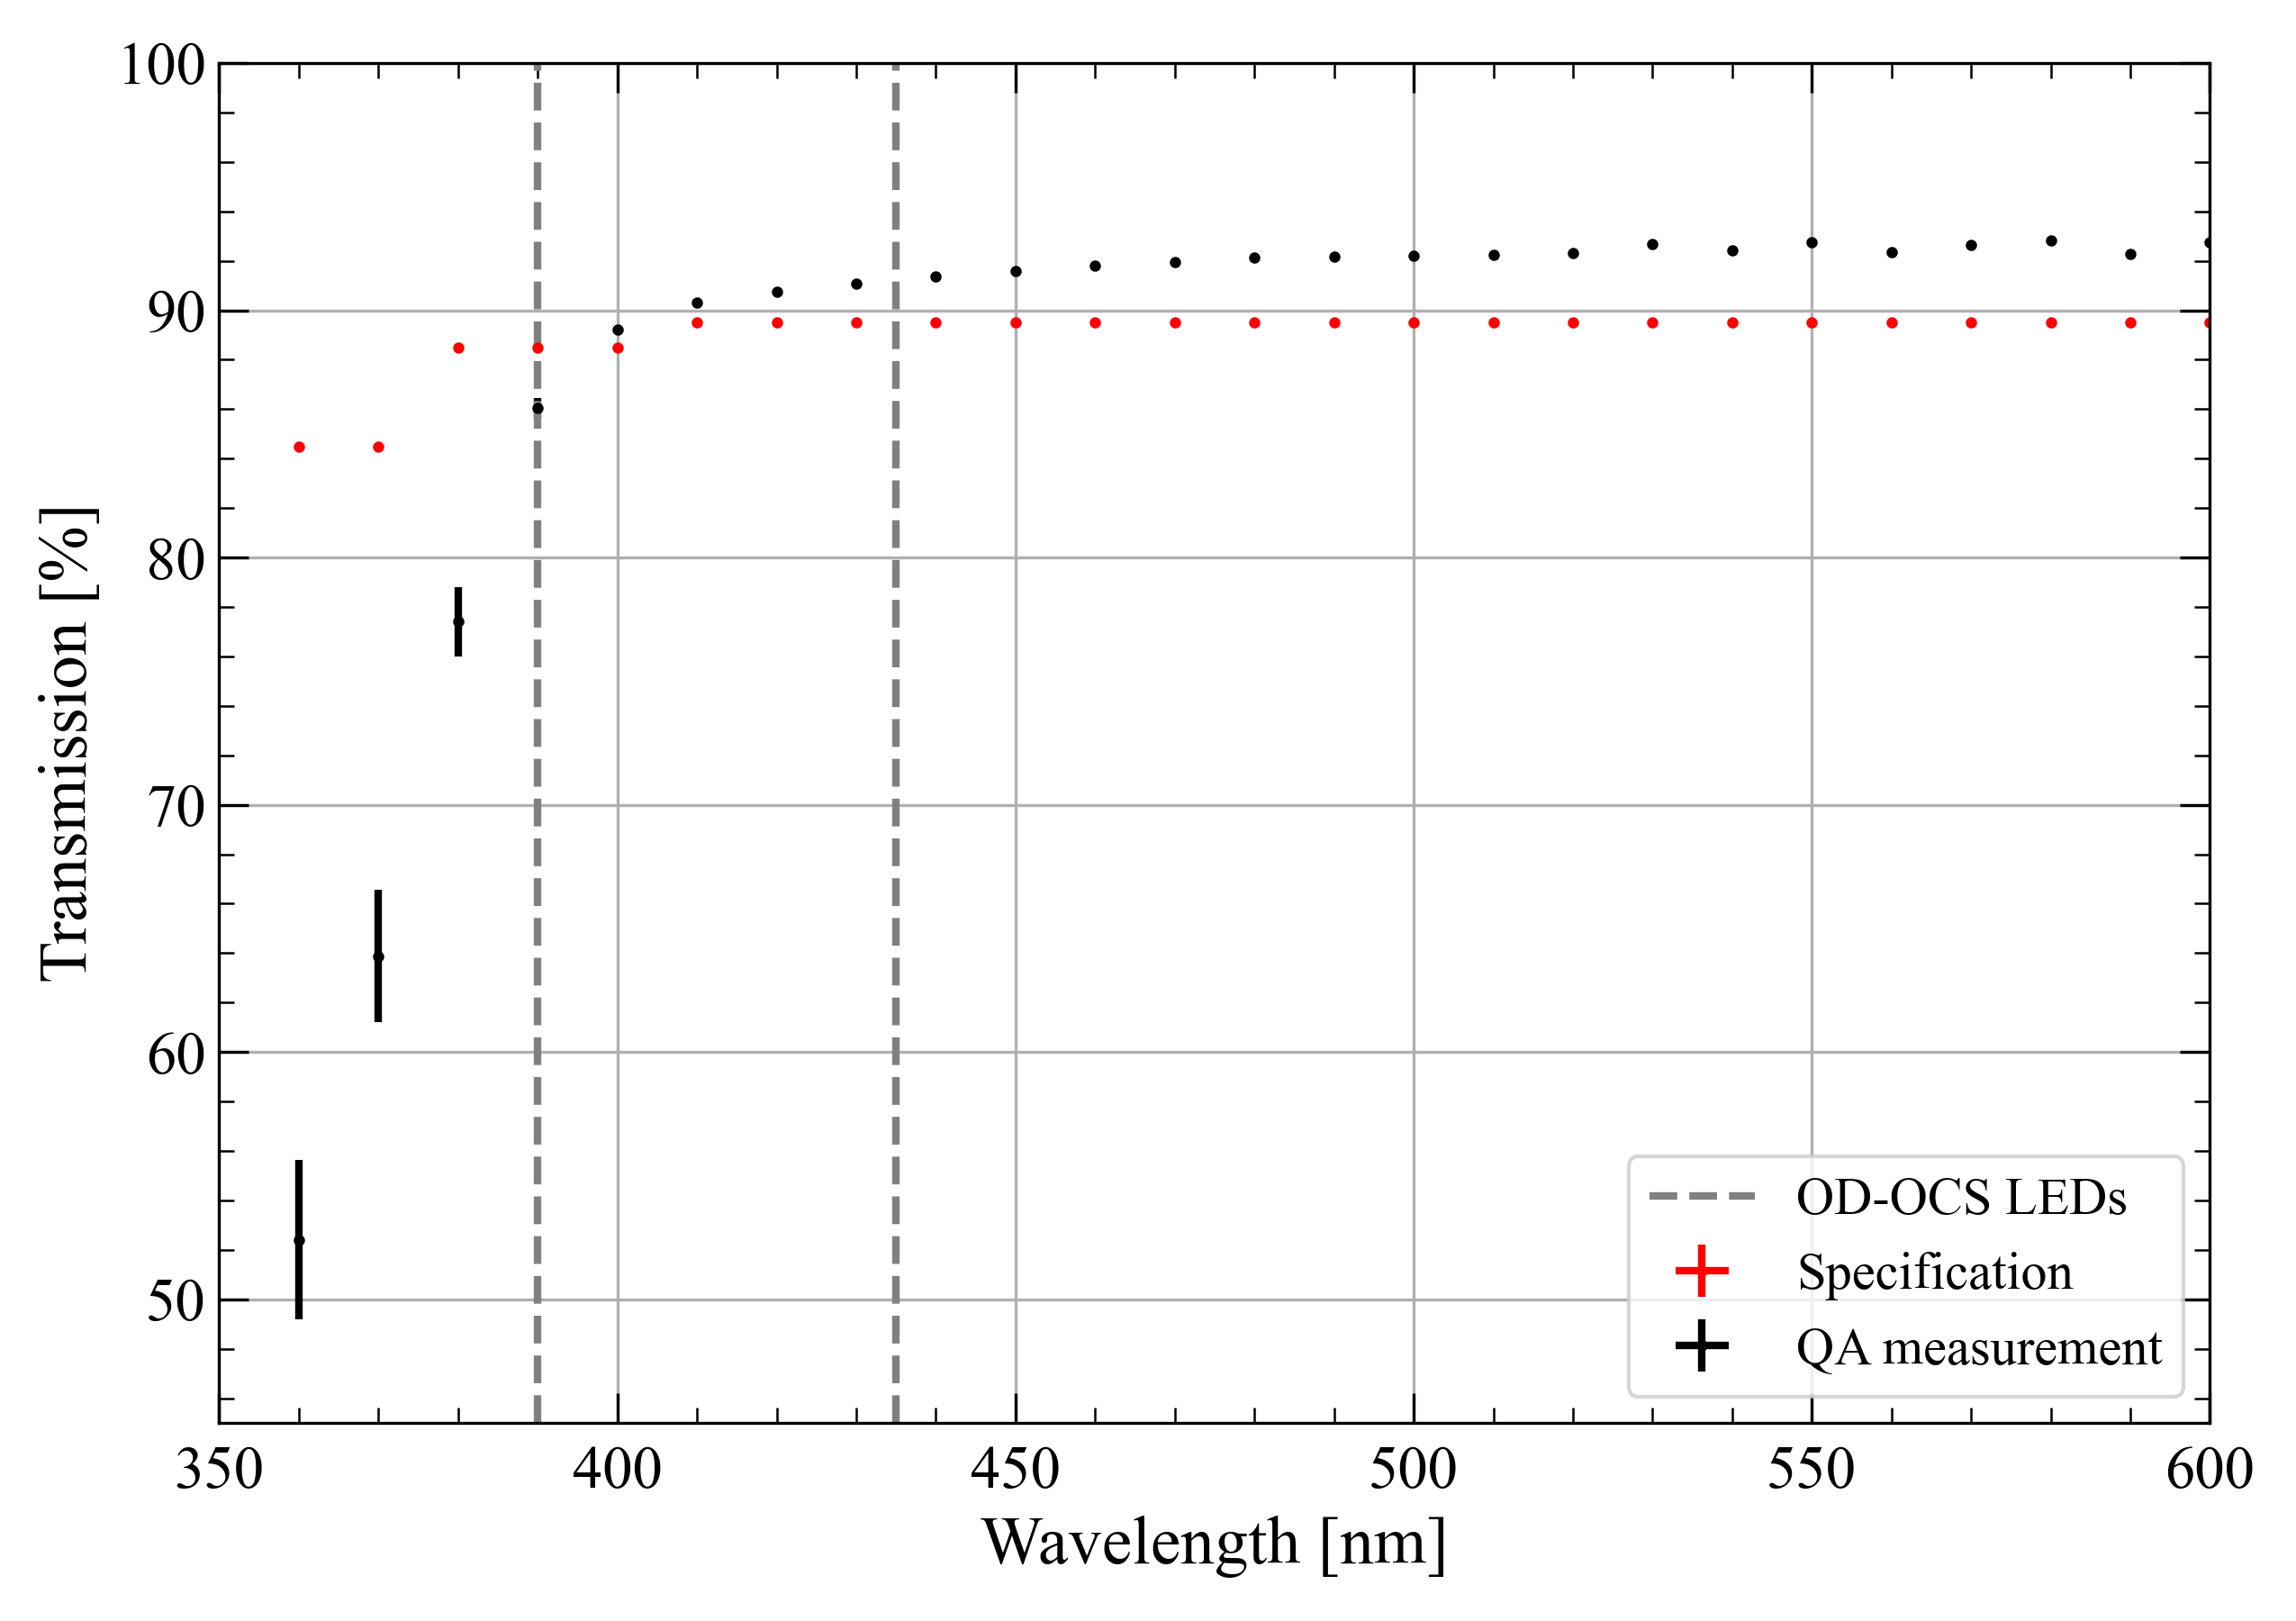
\includegraphics[width=0.8\linewidth]{figures/LZ/T187-XDM-UVT_WAVELENGHT_08252017.png}
    \caption{Quality assurance measurement data taken during the commissioning of the acrylic tanks. The QA measurement data is the average transmission of light at a particular wavelength across 46 points. Vertical lines indicate the 390~nm and 435~nm LEDs with respect to the transmission of light.}
    \label{fig:LZ/AcrylicQA}
\end{figure}
The electronics system which controls the LEDs consists of five Optical Calibration Cards (OCC). Each OCC consists of an FPGA controlled motherboard which houses eight LED pulser boards and two four-channel photodiode boards. Light pulses from the LEDs are divided by a three-way optical coupler: to the injection points in the OD; to the photodiode readout for onboard monitoring; to a monitoring PMT. The layout of the system can be seen in \autoref{fig:LZ/OCSSchematic}.
\begin{figure}[!ht]
    \centering
    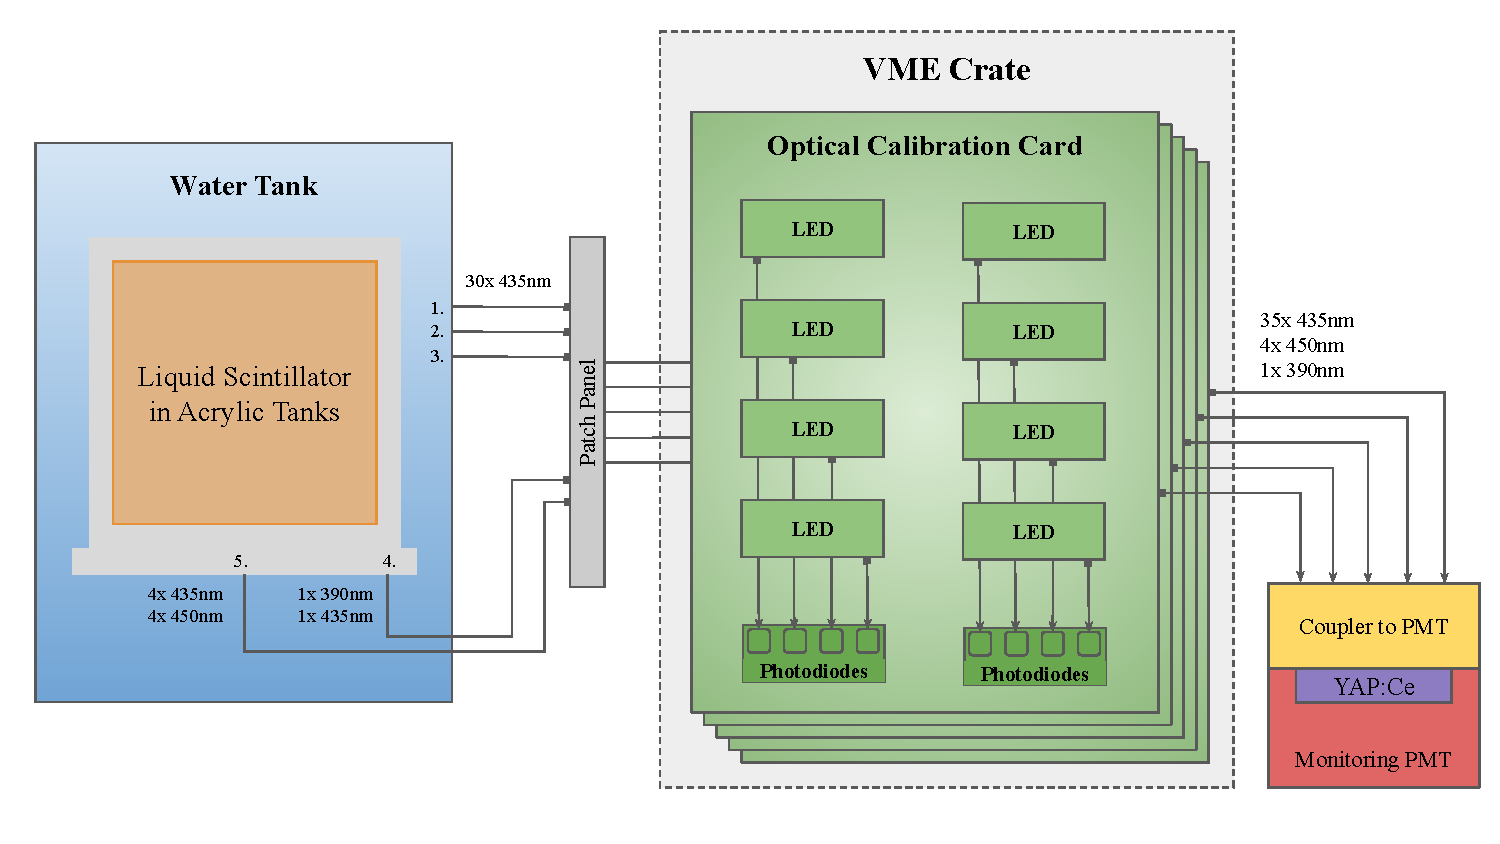
\includegraphics[width=\linewidth]{figures/LZ/OCSSchematics.pdf}
    \caption{A schematic of the OD OCS. An example of one Optical Calibration Card (OCC) is shown with its eight LED pulser boards and two photodiode boards. A total of five OCCs make up the OCS and are powered by a VME crate. Lines with arrows show the paths light takes down various fibres to different positions in the system. Labels 1-3 represent the three heights within the PMT array, while Label 4-5 denote the injection points to monitor the GdLS/acrylic, as shown in \autoref{fig:LZ/OCSPositions}. Adapted from Ref.~\cite{Turner:2021qvi,LZ:2024bsz}.}
    \label{fig:LZ/OCSSchematic}
\end{figure}
The intensity of light is monitored using the onboard photodiode and rack mounted monitoring PMT, which is the same 8-inch Hamamatsu R5912 PMT as used in the OD PMT array \cite{Turner:2021qvi}. The commissioning of this component of the subsystem is covered further in \autoref{chap:ODCommissioning}. The OCS is controlled through LZ's central Slow Control System, allowing a user to define a pulse size/intensity using a graphical user interface \cite{hbirch:thesis}.
The author was a member of the group at the University of Liverpool, who developed the OCS and worked on extensively testing the system during postgraduate studies. The OCS met all design requirements set by LZ \cite{Turner:2021qvi}. Further details of the OCS and the quality assurance testing prior to installation can be found in Ref.~\cite{hbirch:thesis,Turner:2021qvi}.
\section{Calibration systems and sources}\label{sec:LZ/CalibrationSources}
To understand the LZ detector response and its performance, regular calibrations are performed using a variety of methods and sources. Such calibration procedures are used to characterise the energy scale, energy threshold, micro physics of particle interactions, as well as the position and time dependence of the detector responses \cite{LZ:2024bsz}. A summary of the sources, their purpose and their deployment methods is shown in \autoref{tab:LZ/CalibrationSources}.
\begin{table}[!ht]
    \centering
    \caption{A list of calibration source used by LZ for TPC, Skin and OD calibrations along with the purpose and method of deployment. The energy (keV) refers to particle energies relevant for the calibration of LZ and is not a complete list of decay energies. The energies quoted in the parentheses correspond to those of the particle species from the previous column. Adapted from Ref.~\cite{LZ:2024bsz,lkorley:thesis}.}
    \begin{tabular}{lllll}
         \hline\hline
         \textbf{Isotope}&\textbf{Interacting}&\textbf{Energy [keV]}&\textbf{Purpose}&\textbf{Deployment}\\
         &\textbf{Particle}& & & \\
         \hline
         $^{83m}\text{Kr}$ & $\beta, \gamma$ & $32.1/9.4$ &TPC(x,y,z) & Injected\\
         $^{131m}\text{Xe}$& $\gamma$, x-ray & $163.9$ & TPC(x,y,z), Skin & Injected\\
         $^{220}\text{Rn}$& $\alpha,\beta,\gamma$ & Various \cite{Jorg:2023nvl} & Skin, ER Band & Injected\\
         $^{3}\text{H}$& $\beta$ & $0-18.6$ &ER Band & Injected\\
         $^{14}\text{C}$& $\beta$ & $0-156.4$ &ER Band & Injected\\
         $^{241}\text{AmLi}$& $(\alpha,n)$ & $(5638, 0-1500)$ & NR Band, Veto Efficiency & CSD\\
         $^{241}\text{AmBe}$& $(\alpha,n)$ & $(5638, 0-11\times10^{3})$ & NR Band, Veto Efficiency & CSD\\
         %$^{252}\text{Cf}$& Spontaneous Fission & &NR Efficency & External\\
         $^{57}\text{Co}$& $\gamma$ & $122$ &Skin Energy Scale & CSD\\
         $^{228}\text{Th}$& $\gamma$ & $2615$ &OD Energy Scale & CSD\\
         $^{22}\text{Na}$& $\gamma$ & $511, 1275$ &Inter-detector Timing & CSD\\
         $^{52}\text{Mn}$& $\gamma$ & $835$ &Skin Energy Scale & CSD\\
         $^{88}\text{YBe}$& $(\gamma,n)$ & $(1836,152)$ &NR Response & External\\
         $^{88}\text{YMg}$& $n$ & $1836$ & NR Response & External\\
         DD& $n$ & $2460$ & Light and Charge Yields & External\\
         $^{241}\text{Am}$& $\alpha$ & $5638$ &ODOCS Calibration & External\\
         \hline\hline
    \end{tabular}
    \label{tab:LZ/CalibrationSources}
\end{table}
Injected sources consist of gaseous radioisotopes which are injected into the xenon circulation system and in turn into the TPC volume itself. The injection of sources directly into the TPC volume is beneficial for a few reasons. Firstly, as source is injected and allow to mix with the LXe, this allows calibration with spatial uniformity. Secondly, the LXe target is self-shielding so an external low energy source would require a large amount of exposure time to achieve comparable statistics to the injected source. Lastly, monitoring how the injected isotopes mix within the TPC allows LZ to further understand the mixing and flow patterns of background radioisotopes \cite{LZ:2024bsz}. The injected radioisotopes either decay away due to their short-lived nature ($^{83m}\text{Kr}$,$^{131m}\text{Xe}$ and $^{220}\text{Rn}$) whereas the live-lived source, tritiated methane ($\text{CH}_4$), is removed by the hot zirconium getter \cite{LZNIMA}.

Beyond the injected sources, there are external sources which can be separated into two subcategories by their deployment, either using the Calibration Source Deployment system or stand alone deployment method. The CSD lowers neutron and gamma rod sources in three tubes located in the vacuum space between the ICV and OCV \cite{LZNIMA}. Each tube is connected to an independent deployment system which allows sources to be precisely positioned at different depths in the detector. Depending on the depth of deployment, the radioactive source can generate signals in various regions of the OD, TPC, and Skin. The use of various sources at various heights allows for calibration of the detectors' energy scale and the spatial dependence of the energy scale. Inter-detector timing measurements between the three detectors is also carried out using the CSD sources. Understanding time offsets between the detectors is crucial for functioning veto system which is dependent on time based section to remove background events.

Beside the CSD sources, a deuterium-deuterium (DD) neutron generator is used to produced neutrons for TPC calibrations and to cross check veto tagging efficiency (discussed in \autoref{sec:VetoEff/efficiency}). The generator produces 2.45~MeV neutrons which are directed through calibration conduits that pass through the OD acrylic tanks to the OCV. A detailed description the system is provided in Ref.~\cite{LZ:2024bsz}. To understand low energy detection efficiency of the TPC $^{88}\text{YBe}$ and $^{88}\text{YMg}$ photo-neutron sources are used. Both sources are deployed externally through a removing a small acrylic vessel in the OD and replacing it with source assembly. This small vessel is shown in green above the blue top tanks in  \autoref{fig:LZ/ODTanks}.
The final source listed in \autoref{tab:LZ/CalibrationSources} is sealed $^{241}\text{Am}$ within a YAP:Ce crystal and is used within the ODOCS, as described in \autoref{sec:LZ/ODOCS}.

\section{Data acquisition system}\label{sec:LZ/LZDAQ}
Signals produced in the PMTs across the experiment are processed by the data acquisition system. LZ employs a custom FPGA-based Architecture for Data Acquisition and Real time monitoring (FADR) to perform the digitisation and identify events of interest for offline analysis \cite{LZ:2024bvw,Druszkiewicz:2015pcl}. 
Signals first pass through shaping amplifiers which increases signal-noise ratio. At the amplifier stage, the signals from the TPC and OD are split into dual gain outputs to maximize the available dynamic range and extend the range of energies than can be probed by the experiment. The Skin detector has only a single gain output. Following amplification, the analogue signals are digitized with a sample rate of 100~MHz (10~ns samples) using custom built 32-channel digital signal processing boards \cite{Druszkiewicz:2015pcl}. Due to the sheer volume of data that comes from the PMTs Pulse Only Digitisation (POD) methods are employed to reduce the raw waveform volume by a factor of 50 \cite{LZTDR}. The threshold used in this filter is tuned on SPhE data and is set to provide a detection efficiency of $>99\%$ \cite{LZ:2024bvw}. 

During normal operation, event selection is based on multiple trigger sources which can be divided into two categories, \textit{WIMP-search Triggers} and \textit{Calibration Triggers}. When the experiment is in WIMP-search operation the detector based event selection follows the logical OR decision on the list of triggers below:
\begin{itemize}
    \item The TPC S2 trigger. This trigger is based on the S2 filter response from the high gain signal of the TPC top array PMTs.
    \item The Skin S1 trigger. This trigger is based on the S1 filter response of the Skin PMTs and is used to monitor the health of the PMTs in the volume.
    \item The OD S1 trigger. This trigger is based on the S1 filter response of the OD PMTs, specifically the high gain channels. The trigger is used to monitor the health of the PMTs in the volume and for specific OD based physics searches.
    \item A random trigger. This trigger operates with a random rate of $\sim4$~Hz to provide an unbiased sample for monitoring background events and trigger efficiencies. 
    \item The GPS trigger. This trigger runs at exactly 1~Hz and is independent of detector signals, to monitor detector health and FADR performance. 
\end{itemize}
External triggers are used during certain calibrations and are listed below:
\begin{itemize}
    \item DD trigger. This trigger is generated by the neutron generator when the system is pulsed.
    \item LED trigger. Two different LED systems are used to calibrate and monitor the health of the PMTs \cite{LZ:2024bsz}. When the LEDs are fired, a trigger signal is generated.
\end{itemize}
\begin{figure}[!ht]
    \centering
    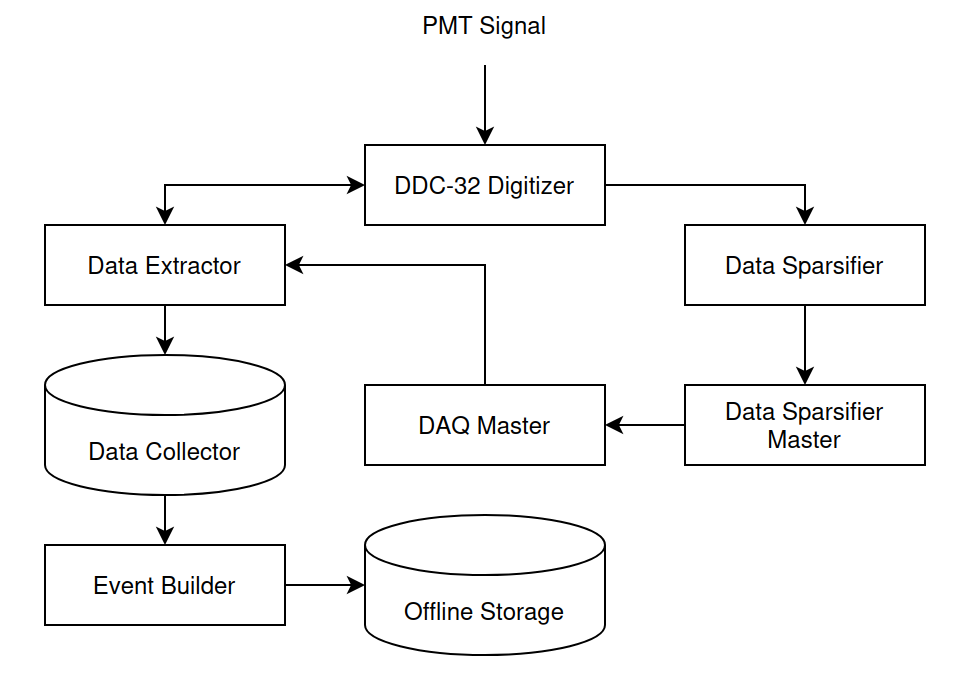
\includegraphics[width=\linewidth]{figures/LZ/LZDAQ.png}
    \caption{A simplified schematic depicting how PMT signals are processed using the LZ DAQ system. Adapted from Ref.~\cite{LZ:2024bvw}.}
    \label{fig:LZ/LZDAQ}
\end{figure}
Results from the POD waveform analysis are passed to the data sparsifiers and grouped by the Data Sparsifier Master (DSM) where a decision is made whether an event has been observed. The DSM informs the DAQ Master and time window is selected for the event and the data is extracted from the digitizers and stored by one of the Data Collectors. A simplified schematic of the LZ DAQ system is shown in \ref{fig:LZ/LZDAQ}, depicting one channel of digital electronics. Event builders take the data which has been temporarily stored on the Data Collectors, organized the data by channel, and assembles full event structures for offline analysis. An in-depth description of FADR can be found at Ref.~\cite{LZ:2024bvw}. 
\section{Simulation techniques}\label{sec:LZ/Simulations}
Simulations of the LZ experiment play a key role understanding the detector and its response. They present several purposes, for example: the calculation of background rates in LZ; the prediction of of sensitivity of the experiment to rare event searches through Profile Likelihood Ratio analysis (PLR); the testing of event reconstruction infrastructure; determining efficiencies of data selection methods. An overview of the LZ simulation framework is shown in \autoref{fig:LZ/LZSimFramework}.
\begin{figure}[!ht]
    \centering
    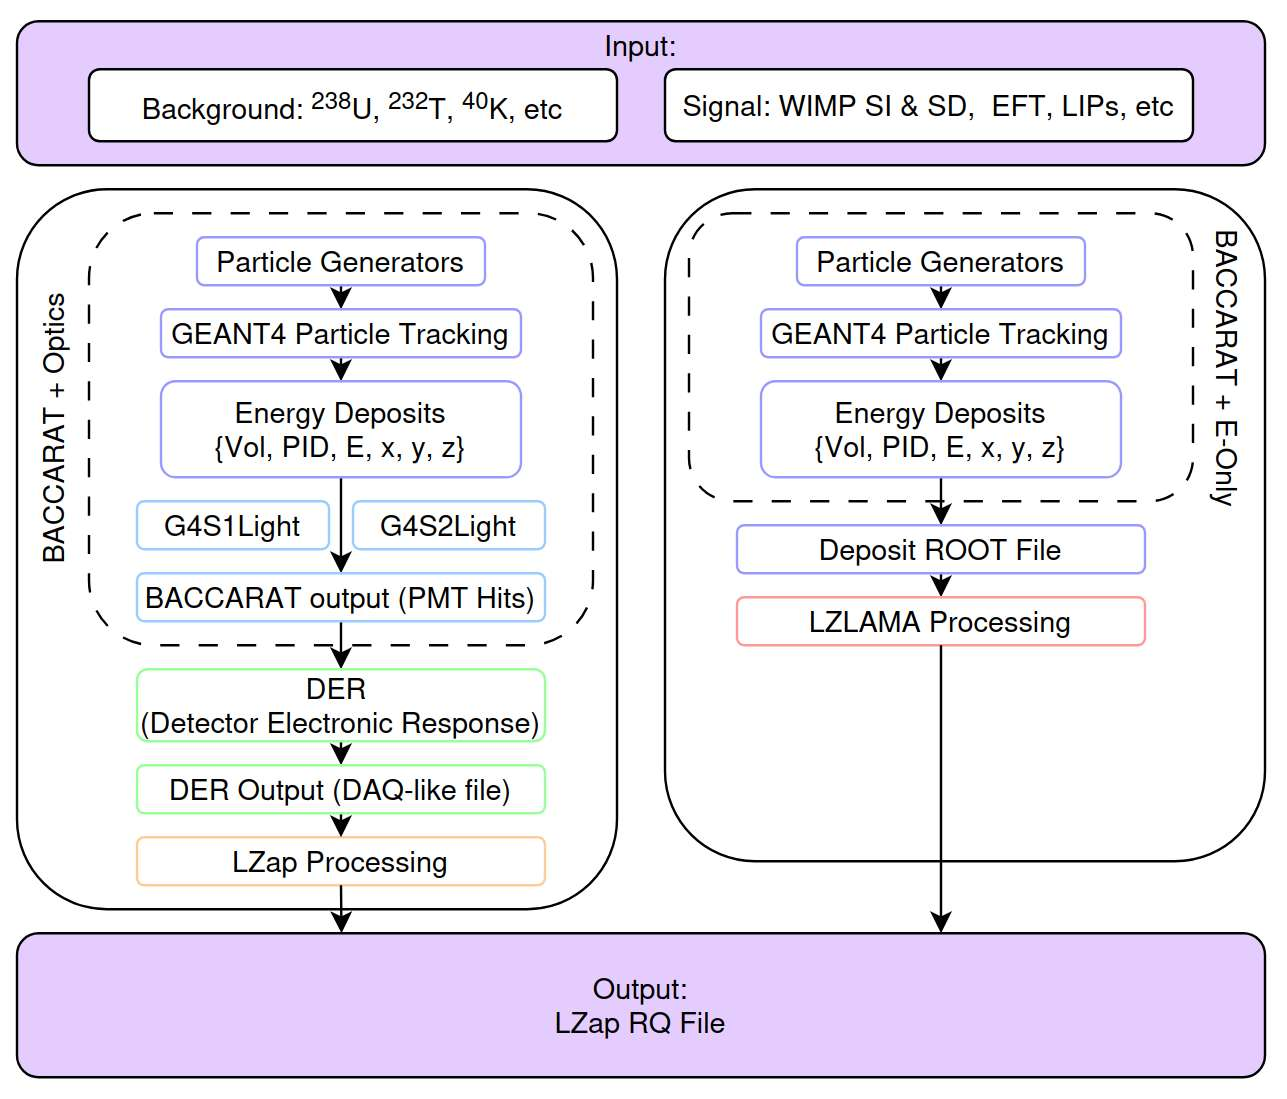
\includegraphics[width=\linewidth]{figures/LZ/LZSimFramework.png}
    \caption{Simulation framework for the LZ experiment. ``Full'' and ``Fast'' simulation chains are shown. Both chains begin with BACCARAT and end with an output LZAP RQ file.}
    \label{fig:LZ/LZSimFramework}
\end{figure}
For all simulations, LZ uses BACCARAT\footnote{\textbf{B}asically \textbf{A} \textbf{C}omponent-\textbf{C}entric \textbf{A}nalogue \textbf{R}esponse to \textbf{A}ny\textbf{T}hing}\cite{LZ_SIMS} package to simulate particle interactions in the detector and this package is built upon the GEANT4 simulation toolkit \cite{GEANT4:2002zbu}. Using GEANT4 along with CAD-Drawing, the LZ experiment is built as a detector geometry. In simulation, a series of inputs can be used to generate particles which are propagated through the detector geometry, with any additional particles being generated from interactions with detector materials. GEANT4 is used to track the particles and identifies the interaction points. From there, two separate chains exist for interpreting this information, \autoref{fig:LZ/LZSimFramework}.

The ``Fast'' chain, seen on the right of \autoref{fig:LZ/LZSimFramework}, records energy deposits in the detector and passes them to LZLAMA for processing. LZLAMA consists of two primary packages, the Noble Element Simulation Technique (NEST) to process interactions in the xenon space and DICEBOX to process interactions with the OD. NEST provides the expected conversion of energy to scintillation photons and ionization electrons based on empirical models developed using experiment measurements \cite{NEST1}. The DICEBOX toolkit is empolyed to handle interactions between neutrons and their capture on Gd as GEANT4 has difficulty conserving Q-value and multiplicity of the gamma emissions from the neutron capture. Energy deposits in other volumes are handled by GEANT4. LZLAMA outputs a ROOT file which has the same reduced-quantity (RQ) format as data processed using LZ's custom processing tool, LZAP \cite{LZ_SIMS}, which performs pulse and event reconstruction.

The second, ``Full'' chain, enables full simulation of optical processes throughout the entire detector including VUV photons and ionisation electrons that are produced in the xenon and scintillation light generated in the OD. Another custom LZ software package, Detector Electronic Response (DER), is used to translate PMT hits in the BACCARAT output into waveforms. The DER simulates the analogue front-end electronics of LZ to produce waveforms, written in an identical format to the true LZ DAQ, \autoref{sec:LZ/LZDAQ}. A number of physical processes are incorporated into the DER to create realistic waveforms including: a PMT response model, gain, quantum efficiency, double photoelectron probability, dynode effects, dark rate, and afterpulsing. This chain is more computationally intensive but it allows for a more realistic, event-by-event analysis. The output from the DER is processed by LZAP to produce RQ-structured files to be analysed much like real data.
A complete review of the LZ Simulation framework can be found at Ref.~\cite{LZ_SIMS}.

\section{Assembly and operation of the LZ detector}\label{sec:LZ/LZAssembly}
During the past six years whilst the author has collaborated on the LZ Experiment, a significant portion of that time has been spent on-site at SURF working on the assembly, commissioning and operation of the LZ Detector. These efforts began with the installation of the OCS electronics and an in-situ-calibration of the LED system, this work is detailed extensively in Ref.~\cite{hbirch:thesis}.
\begin{figure}[!ht]
     \centering
     \begin{subfigure}{0.47\textwidth}
         \centering
         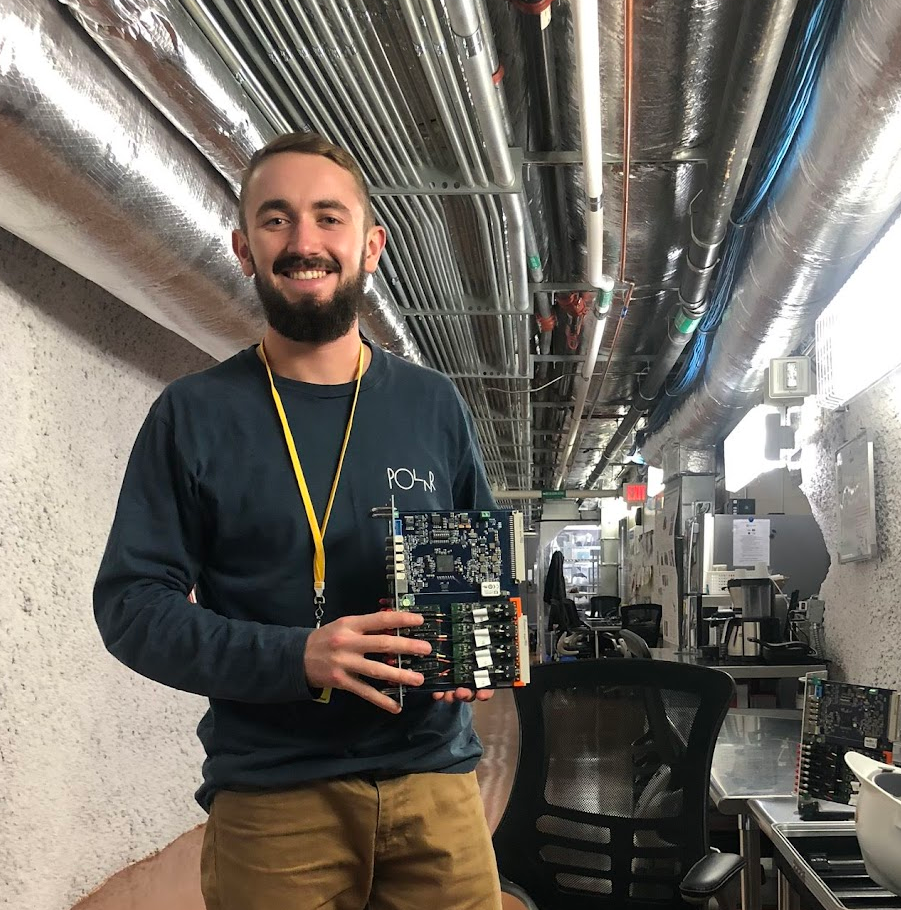
\includegraphics[width=0.95\textwidth]{figures/LZ/OCSMotherboardCC.png}
         \label{fig:LZ/Gonk0}
     \end{subfigure}
     %\hfill
     \begin{subfigure}{0.47\textwidth}
         \centering
         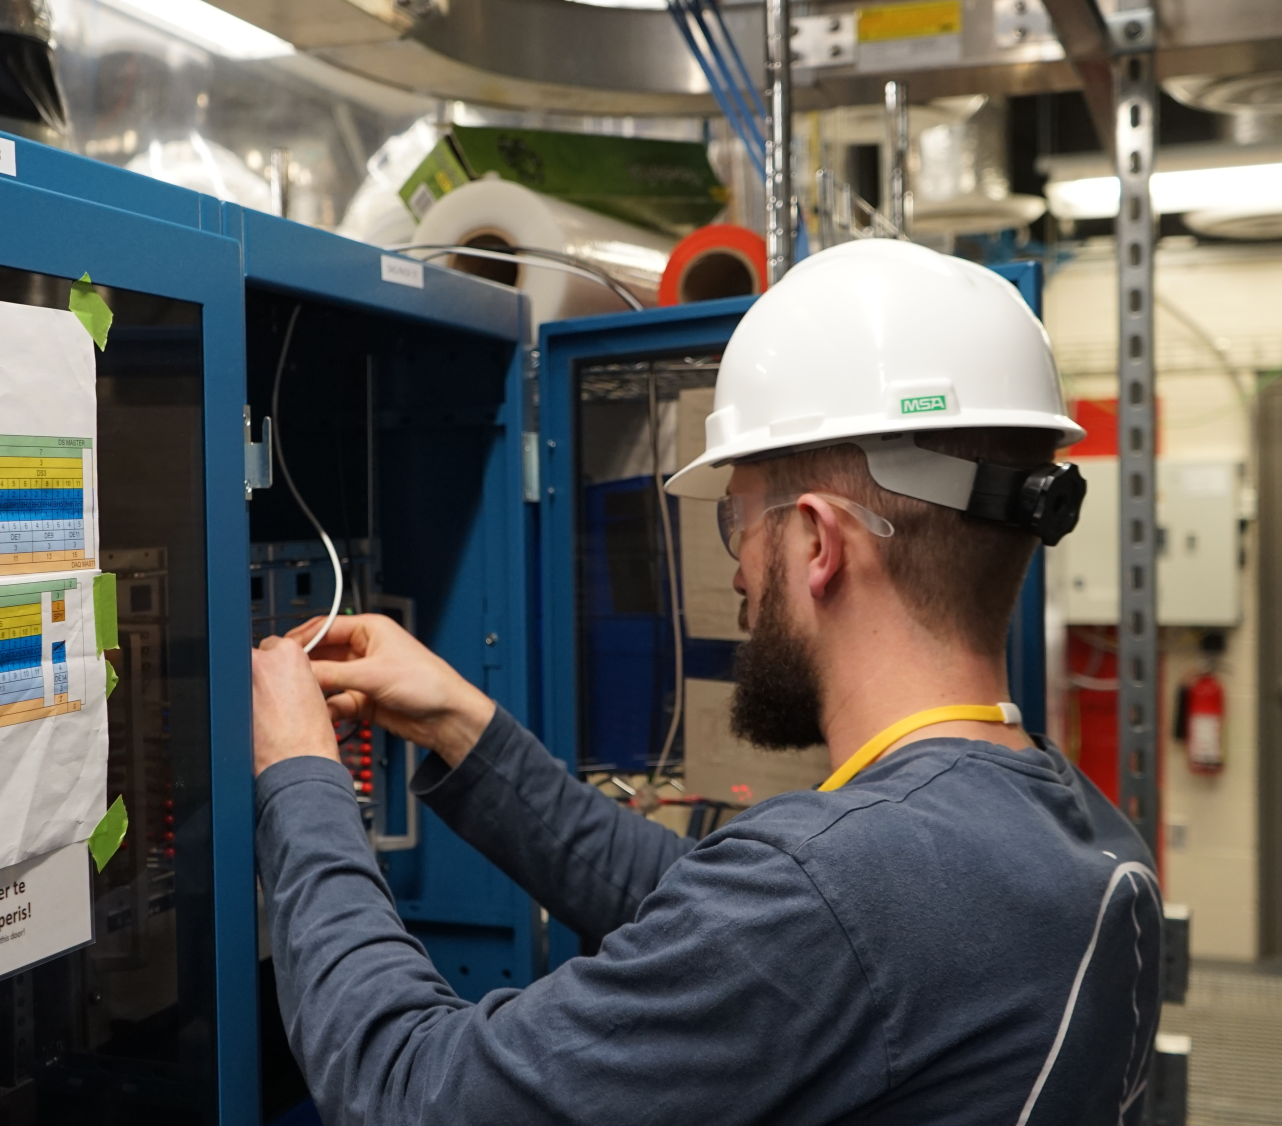
\includegraphics[width=\textwidth]{figures/LZ/OCSElectronicsInstallation.png}
         \label{fig:LZ/Gonk1}
     \end{subfigure}
     \caption{OD OCS electronics installation. \textbf{Left:} The author standing in the common corridor at the Davis Campus holding an OCC prior to the OCS electronics installation. \textbf{Right:} The author making serial connections between the front planes of the OCS OCCs within the electronics racks.}
\end{figure}
\chapter{Outer Detector Commissioning and Monitoring}\label{chap:ODCommissioning}
\section{OD PMT Calibration}
As discussed in \ref{sec:LZOD}, the primary purpose for the LZ Outer Detector is to detect neutron interactions which have coincident signals within the TPC. The source of most of the neutron background is from the ($\alpha$, n) process in material surrounding the edges of the xenon. A neutron will enter the TPC and then scatter out. The neutron can traverse the intervening material and then thermalize and capture on either the Gadolinium or the Hydrogen in the scintillator mixture or recoil off the protons in the scintillator. When the neutron recoils off the proton, energy depositions of $\sim$100~keV are produced \cite{LZNIMA}. The pulses of light detected in the PMTs for such low energy interactions are $\sim$15 photons in size and require the PMTs to be calibrated to a single photon sensitivity. Understanding the response of the PMTs is key to measuring single photon sensitivity and in turn reconstructing the gain of the PMTs. A model of photomultiplier response is presented in Ref.\cite{BELLAMY1994468} which will be described below.
\subsection{Single Photo-electron Response Model}\label{sec:SPhEResponse}
The PMT is considered to be an instrument which consists of two independent parts:
\begin{itemize}
    \item A photo-cathode where photons are converted into electrons
    \item An amplified which amplifies the initial charge (dynode system)
\end{itemize}
The model assumes that the number of photons incident on the PMT and subsequently the photo-cathode is a Poisson distributed variable. Only a fraction of the photons are converted to photo-electrons, this is the quantum efficiency of the PMT and is a random binary process ($\sim~25\%$ for the OD PMTs). The photo-electrons are then guided towards the first dynode by an electric field in which $\mathcal{O}(100\%)$ photo-electrons complete this process. The convolution of the Poisson and binary process results in a Poisson distribution:
\begin{equation}\label{eqn:SPEPoiss}
    P(n;\mu)=\frac{\mu^{n}e^{-\mu}}{n!},
\end{equation}
where $\mu$ is the mean number of photo-electrons collected at first dynode, $P(n;\mu)$ is the probability that $n$ photo-electrons are observed for a mean $\mu$.
The photo-electron is then amplified by the dynode system, which for the OD PMTs is a series of 10 dynodes. The amplification of the dynode system to determined by the voltage distribution across the dynode and it is tuned on a PMT-by-PMT basis to achieve a gain of $\mathcal{O}(10^6)$. The cascade of photo-electrons produced from the amplification is collected at the anode of the PMT and a voltage is measured as a pulse. The area of the pulse corresponds to number of electrons incident on the anode and is Gaussian distribution:
\begin{equation}\label{eqn:SPEGauss}
    G_n(x)=\frac{1}{\sigma_1\sqrt{2n\pi}}exp\biggl(-\frac{(x-nQ_1)^2}{2n\sigma_1^2}\biggl),
\end{equation}
where $x$ is the variable charge, $Q_1$ is the mean value of the charge outputted from the amplification at the dynode, $\sigma_1$ is the standard deviation of the charge amplification.
The ideal response an ideal PMT, $S_{ideal}$, can be described simply by convoluting \autoref{eqn:SPEPoiss} and \autoref{eqn:SPEGauss} together:
\begin{equation}
    \begin{split}
    S_{ideal}(x) & = P(n;\mu)\otimes G_n(x) \\
    & = \sum^\infty_{n=0}\frac{\mu^{n}e^{-\mu}}{n!}\frac{1}{\sigma_1\sqrt{2n\pi}}exp\biggl(-\frac{(x-nQ_1)^2}{2n\sigma_1^2}\biggl),
    \end{split}
    \label{eqn:PoisPlusGauss}
\end{equation}
the model is summed from 0 photons to an arbitrary upper limit \cite{BELLAMY1994468}.
\subsection{Single Photo-electron Calibration}
To calibrate the OD Single Photo-electron (SPhE) response, light is injected into the OD using the ODOCS. The optimal intensity of light to induce a SPhE response was chosen during the commissioning of the OD following the PMT installation in 2021. Details of the optimisation can be found in Ref.\cite{edfraser:thesis}.

Due to the complex geometry of the OD, the central row fibres were chosen as the injection points, position 2 in \autoref{fig:OCSPositions} (central row). Light injected from the central row fibres pass through the SATs and reflects back of the Tyvek\textregistered\ layer which covers the OCV.
Light injected from position 1 has the ability to pass direct through the TATs. Light injected from position 3 would be reflected within the BATs due to Tyvek\textregistered\ layers which was placed between the three acrylic tanks to cover foam which was needed to displace water. This later design decision was to increase light collection. Irregular gaps between BATs are present due to differences in moulding during construction of the BATs.

The OCS in configured so that 1000~photons are emitted from the end of the fibre. Due to attenuation of light in the fibre, 2000~photons must be emitted by the LEDs to account for a factor of two attenuation. For each injection of light, one of the 10 central row fibre emits 200,000~pulses at a 700~Hz injection rate. The rate of pulses injected was determined to not overload the LZ DAQ.

For ease of repeated measurement, an analysis module for the OD SPhE was developed to be used in conjunction with the LZ \textbf{P}hysics \textbf{RE}adiness \textbf{M}onitor (PREM) \cite{LZTDR}. The analysis module contains a selection to identify the OCS pulse and differentiate it from the background light seen in the OD. It be seen in \autoref{fig:ODSPhE_TimingSelection} that the OCS pulses are distributed around a peak at 560~ns after the trigger (which corresponds to 0~ns in \autoref{fig:ODSPhE_TimingSelection}). A selection of pulses with occurred between 500~ns and 700~ns after the DAQ was triggered by the OCS was chosen as an appropriate set of bounds for the timing selection to identify the OCS pulse. A PMT Coincidence requirement was also imposed to improve the purity of the selection as pulses with a coincidence greater than 1 PMT would likely not include any afterpulses which could mimic an OCS pulse.

\begin{figure}[ht!]
    \centering
    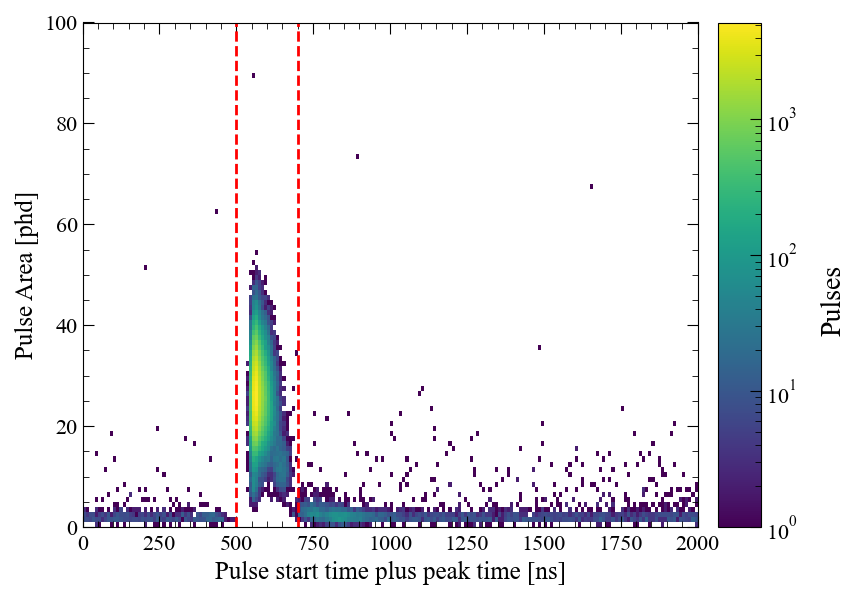
\includegraphics[width=0.8\linewidth]{figures/ODCommissioning/TimingVsPulseArea_2us.png}
    \caption{The response of the OD PMTs to 200k injections of 2000 photons during a monthly SPhE measurement. The pulse area is plotted against the start time of the pulse relative to the trigger plus the peak time relative to the start of the pulse. The OCS pulses are distributed around a peak of 560~ns. The two vertical dashed red lines indicate the inclusive timing selection criteria.}
    \label{fig:ODSPhE_TimingSelection}
\end{figure}

To measure the OD PMT's SPhE response \autoref{eqn:PoisPlusGauss} was used to fit the channel pulse area distributions. A two-stage fitting procedure was employed to account for the monthly variation in SPhE size across all 120 OD PMTs. The first stage of the procedure, only the single SPhE peak is fitted. Initially during commissioning, the starting value for $-\mu$ was determined by estimating the proportion of events in which no photon would be measured by the PMT. The mean and standard deviation (StD) of the histogram was used as starting values for components of the initial fit. The normalisation was taken to be the area beneath the curve between mean/4 and 6$\times$mean. The range in which to apply the fit was determined using the peak and defined from mean $\pm$ (Std/mean). In the second stage of the fitting procedure, the parameters from the initial fit were used as starting parameters to a fit of the multiple SPhE distribution. The range in which to apply the second stage fit was from mean - StD to mean + 3 StD. For each run only one fibre is used to inject light resulting in a small percentage of bad fits across the 120 PMTs depending on the particular fibre being used relative to the PMT of interest. To filter out such bad fits, only fits with $\chi^2/\text{ndf}<3$ were recorded for further analysis.

An example histogram and fit can be seen in \autoref{fig:ODSPhEDists}. It can be seen that the OD PMTs exhibit the expected response to SPhE as discussed in \autoref{sec:SPhEResponse}

\begin{figure}
     \centering
     \begin{subfigure}[b]{0.47\textwidth}
         \centering
         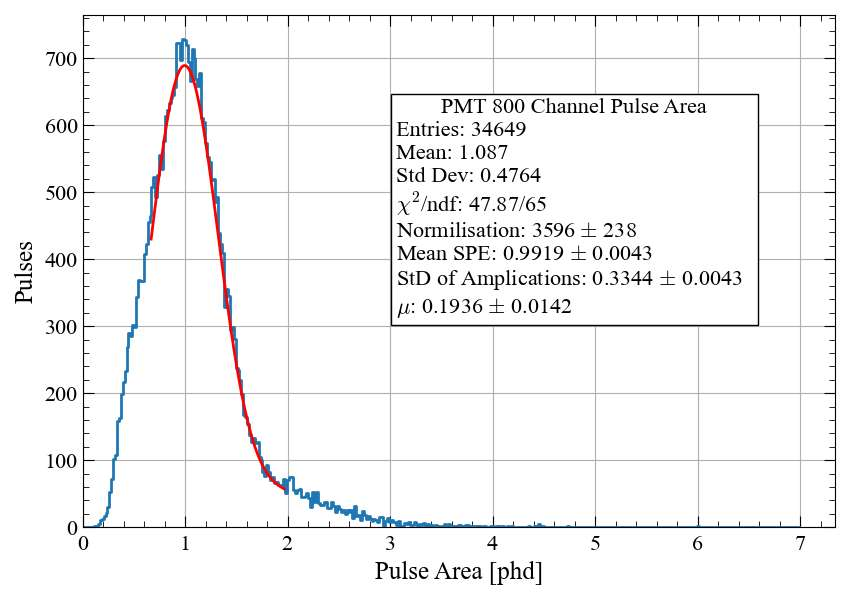
\includegraphics[width=\textwidth]{figures/ODCommissioning/PMT800_PulseArea_Distribution.png}
         \caption{}
         \label{fig:ODSPhE_phd}
     \end{subfigure}
%     \hfill
     \begin{subfigure}[b]{0.47\textwidth}
         \centering
         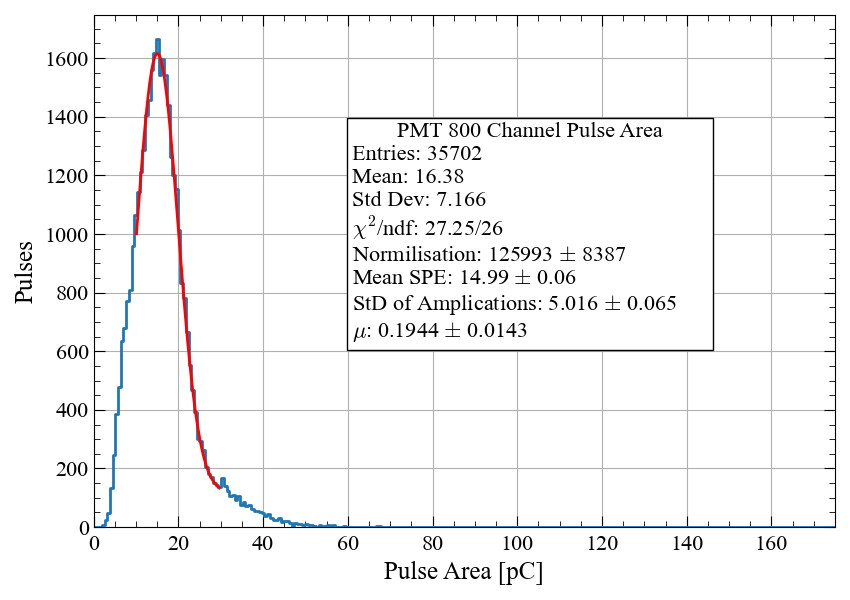
\includegraphics[width=\textwidth]{figures/ODCommissioning/PMT800_PulseArea_Distribution_pC.png}
         \caption{}
         \label{fig:ODSPhE_pC}
     \end{subfigure}
        \caption{Pulse area distributions of PMT 800 from 200k OCS injections of 2000 photons during OD SPhE measurement. \textbf{Left:} Reconstructed pulse area measured in photons detected. \textbf{Right:} Pulse area taken from the area measured in the raw waveform in mVns, and converted to pC by dividing by the $50~\Omega$ termination at the amplifier. The fit applied in red is \autoref{eqn:PoisPlusGauss} and the constants can be seen in the respective statistics boxes on each plot.}
        \label{fig:ODSPhEDists}
\end{figure}
An example PMT calibration is outlined below for PMT 800. The mean Gaussian response is (0.9919 $\pm$ 0.0043) phd and (14.99 $\pm$ 0.06) pC. The SPhE calibration constant used to process the raw data is reconstructed by dividing the SPhE response measured in mVns by the SPhE response measured in phd, which in this case for PMT 800 is 753.9~mVns. These three values together are stored in the PREM database. In a secondary analysis stage, the measured SPhE area and calibration constant are combined to get the correct SPhE constant in mVns which in this example is 748.5~mVns. The average is taken of the corrected SPhE constant for all 10 measurements corresponding to the 10 central row OCS fibre injections. The new SPhE constant is then transferred to the LZ Conditions database along with the data and time period for which this constant is valid for. As LZ then continues to collect data, the raw pulse area measured in mVns is converted to phd by dividing the raw area by the constant. Examples of the variation in measured SPhE in both phd and mVns across all 120 PMTs is shown in \autoref{fig:SPhEValues_phd} and \autoref{fig:SPhEValues_pC}.
\begin{sidewaysfigure}[ht!]
    \centering
    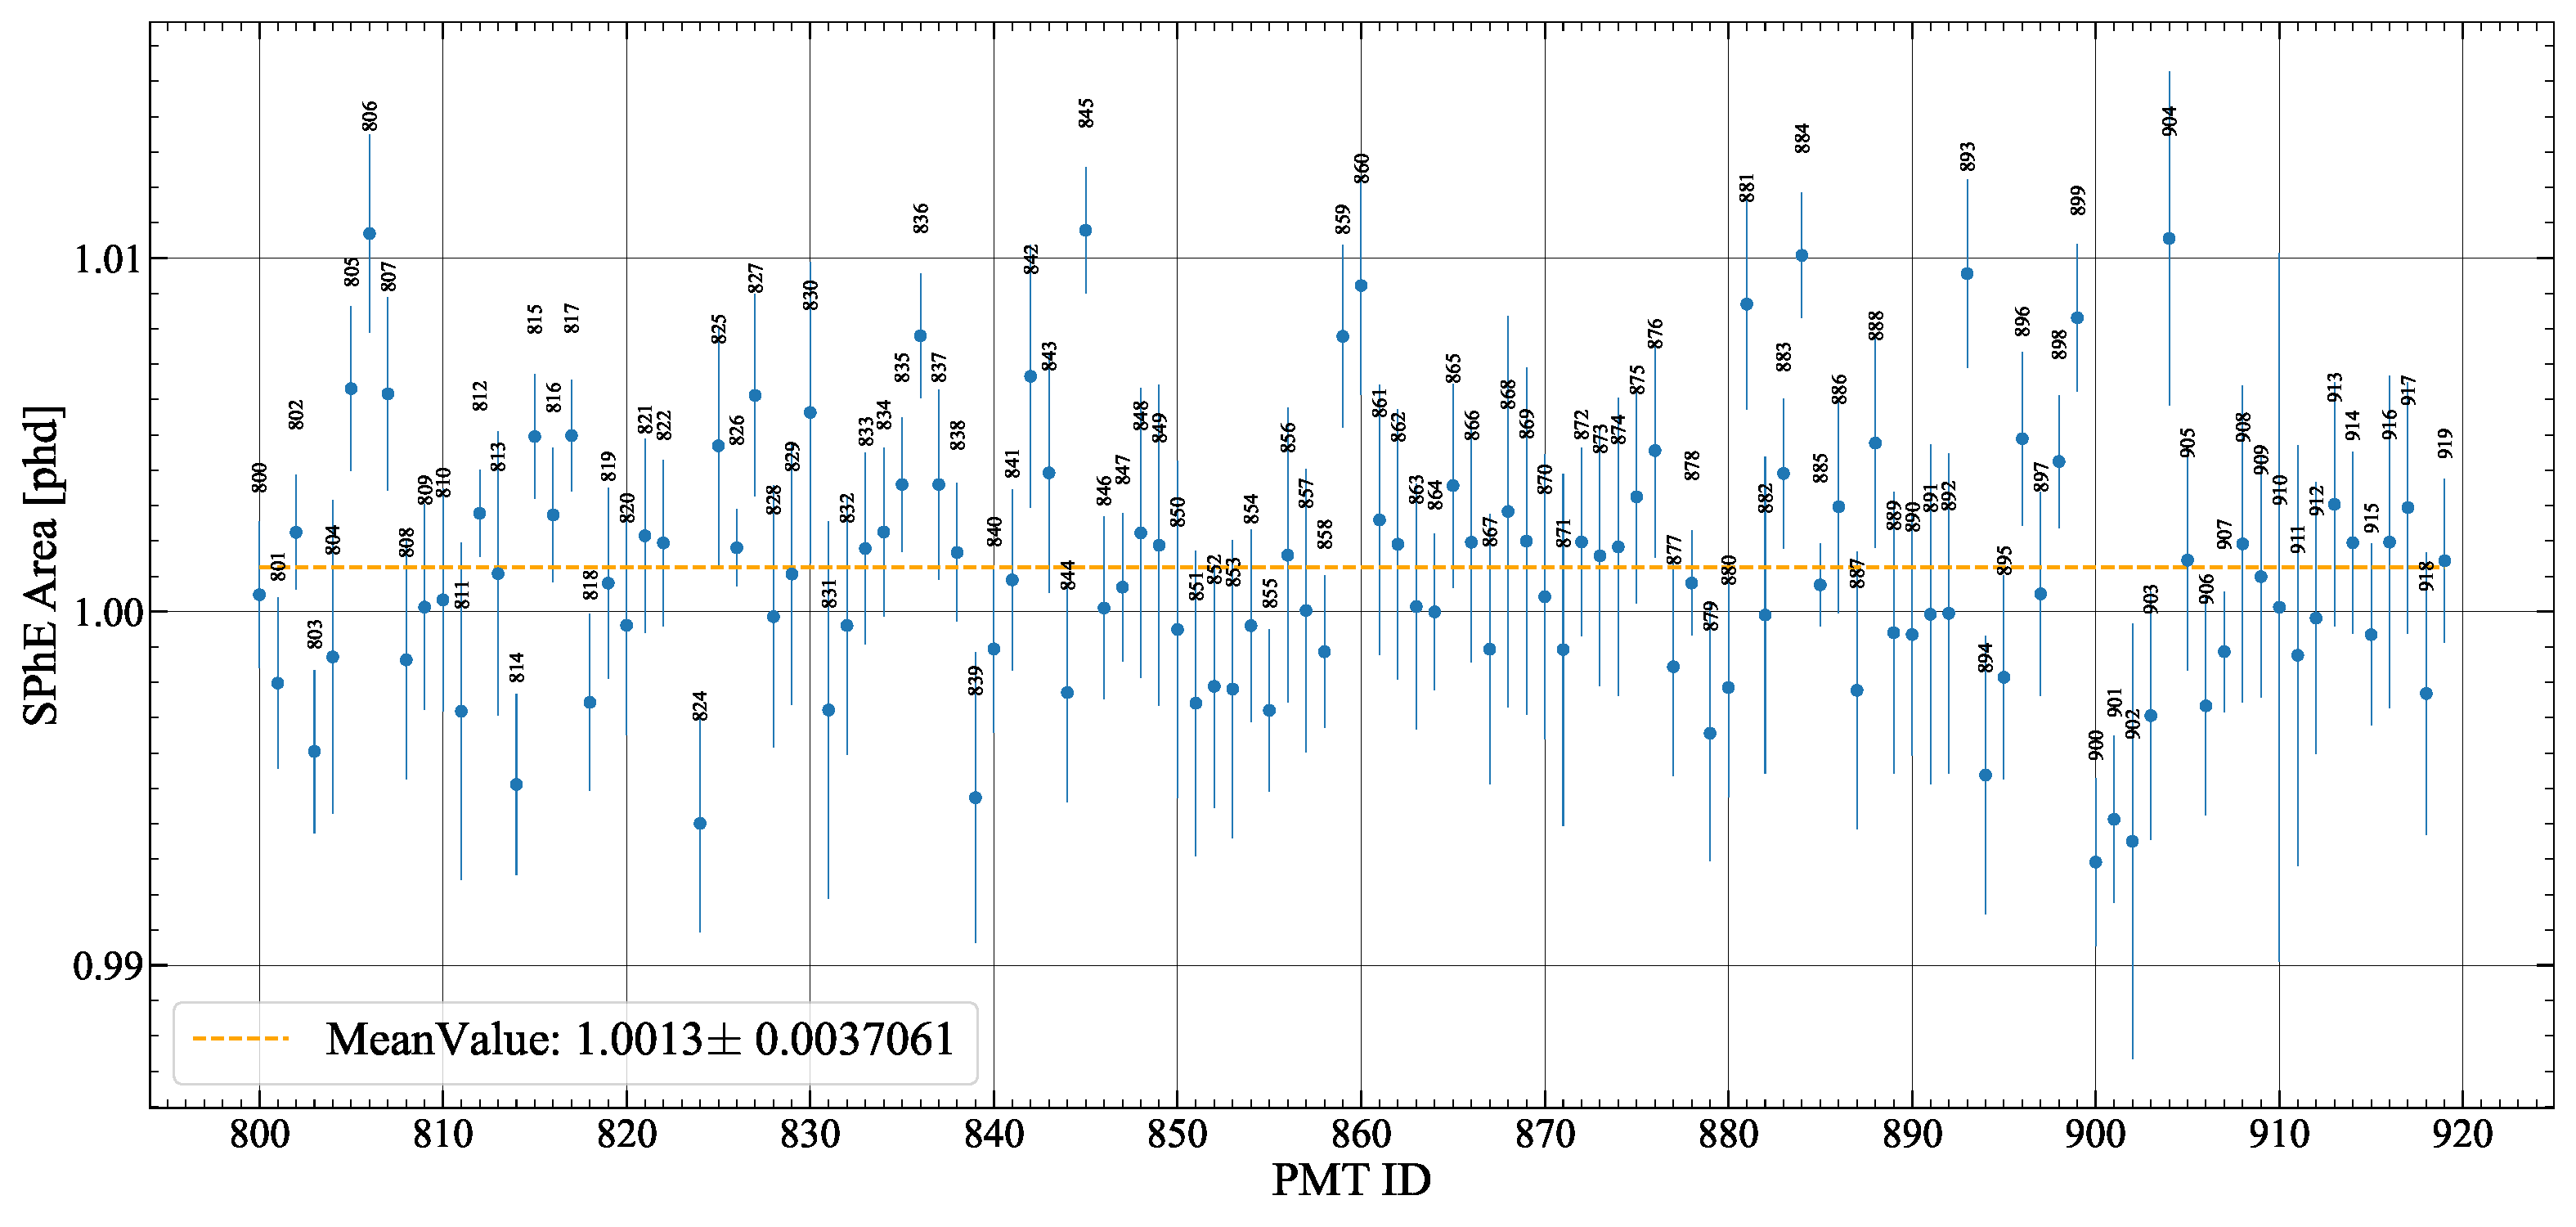
\includegraphics[width=\textwidth]{figures/ODCommissioning/SPHE_phd_2024-7-10.pdf}
    \caption{A scatter plot of the OD SPhE Area size measured in phd versus PMT ID for each OD PMT from a measurement taken on July 10th 2024.}
    \label{fig:SPhEValues_phd}
\end{sidewaysfigure}
\begin{sidewaysfigure}[ht!]
    \centering
    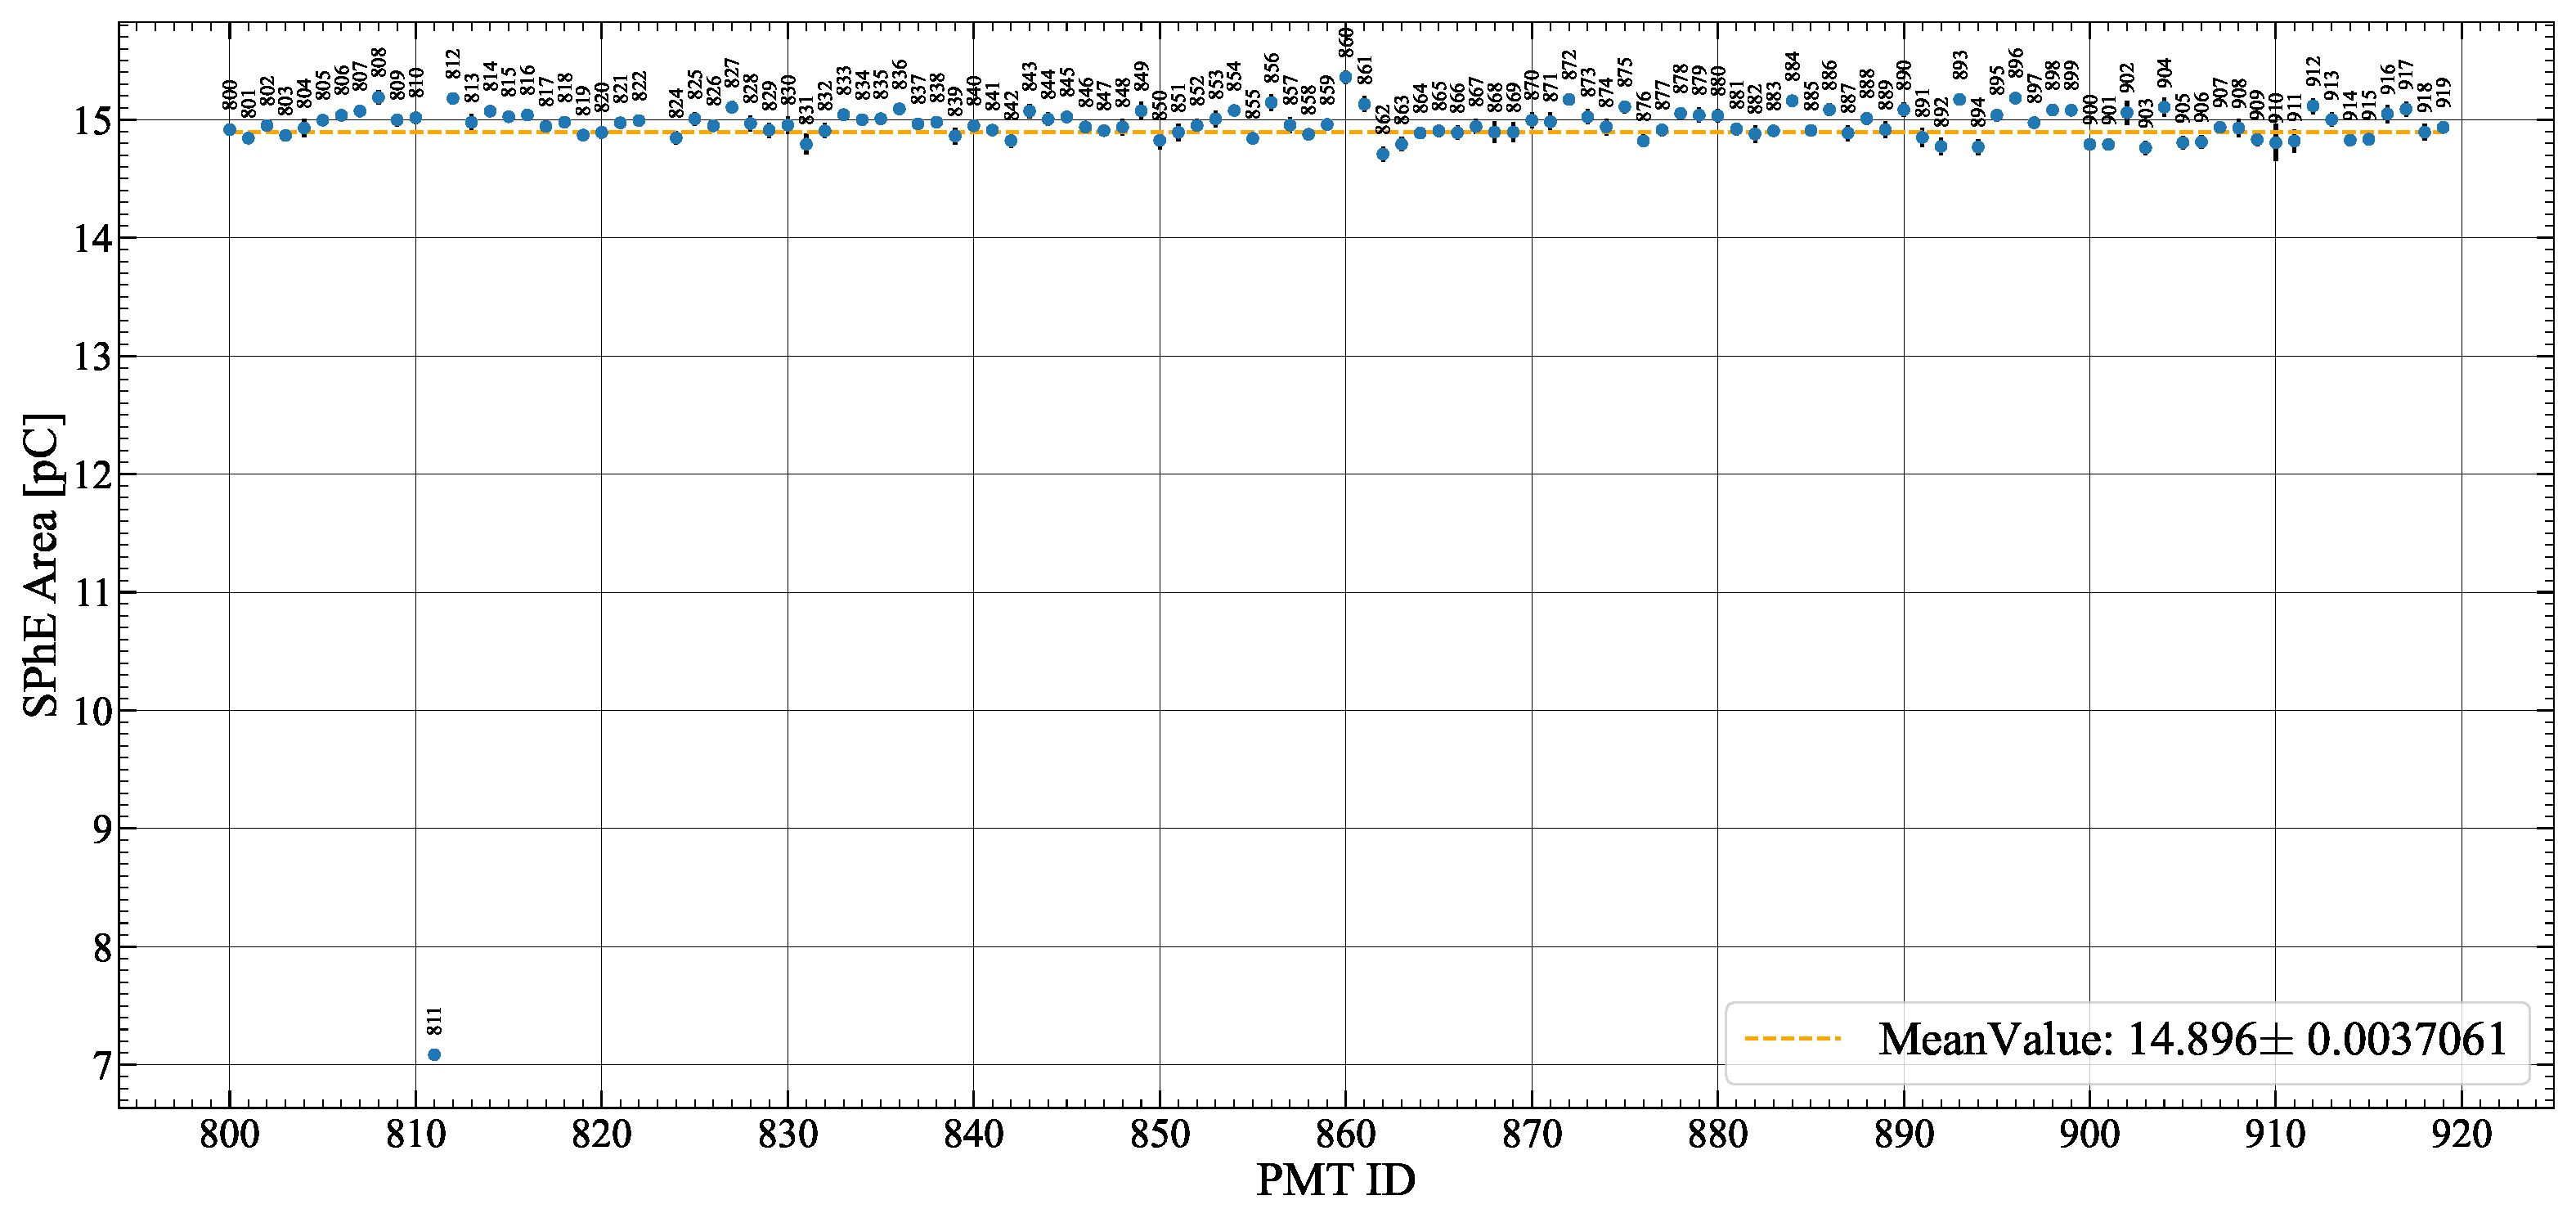
\includegraphics[width=\textwidth]{figures/ODCommissioning/SPHE_pC_2024-7-10.pdf}
    \caption{A scatter plot of the OD SPhE Area size measured in mVns versus PMT ID for each OD PMT from a measurement taken on July 10th 2024.}
    \label{fig:SPhEValues_pC}
\end{sidewaysfigure}


\section{Reconstructed Gain}
So far it has been shown that understanding how the signal from a PMT relates to the amount of light incident on the face of the PMT is key to measuring the energy deposited by particles traversing the detector. The amplification of the photoelectrons produced through the dynode series is known as the PMT's `Gain'. The SPhE Calibration Constant can be converted to understand the gain of the PMT by dividing by the following terms, $e\times44\times50\times10^{12}$, where e is the charge of an electron, $44~\text{V}_{\text{d}}$ is the total voltage division factor across all 10 dynodes in the PMT \cite{HamamatsuR5912}, 50~$\Omega$ is the termination impedance to eliminate signal reflections in the cable \cite{LZ:2024bvw}, $10^{12}$ accounts for the change with the unit prefixes on voltage and time. Using the example case from the previous section, PMT 800 had an average measured SPhE area of 748.5~mVns based on 10 OCS measurements on February $12^{\text{th}}$ 2025 which results in a reconstructed gain of $2.12\times10^6$.

During the commissioning of the Outer Detector PMT system, a target gain of $1\times10^{7}$ initially established based on the operating gain recommended by Hamamatsu Photonics \cite{LZTDR,HamamatsuR5912}. During the OD PMT QA the gain was reduced to $2\times10^{6}$ due to high rates of sub-SPhE noise. Dark rates measurements made during the QA stage exhibited significantly higher rates than the expected 1~kHz dark rate measured in off-site testing. This issue was problematic as spikes up 20~kHz were observed in some cases resulting in the LZ DAQ to crash. Final voltages corresponding to $2.1\times10^{6}$ were determined in October 2021 so that all PMTs achieved the target gain of $2\times10^6$ with $<10~\%$ difference across 119 PMTs. One exception was PMT 811, whose voltage was further reduced in January 2022 resulting in a gain of $1\times10^6$ to reduce the rate of sub-SPhE pulses.
An example scatter plot of gain versus PMT ID is shown in \autoref{fig:ODPMTGain_2024-7-10}

\begin{sidewaysfigure}[ht!]
    \centering
    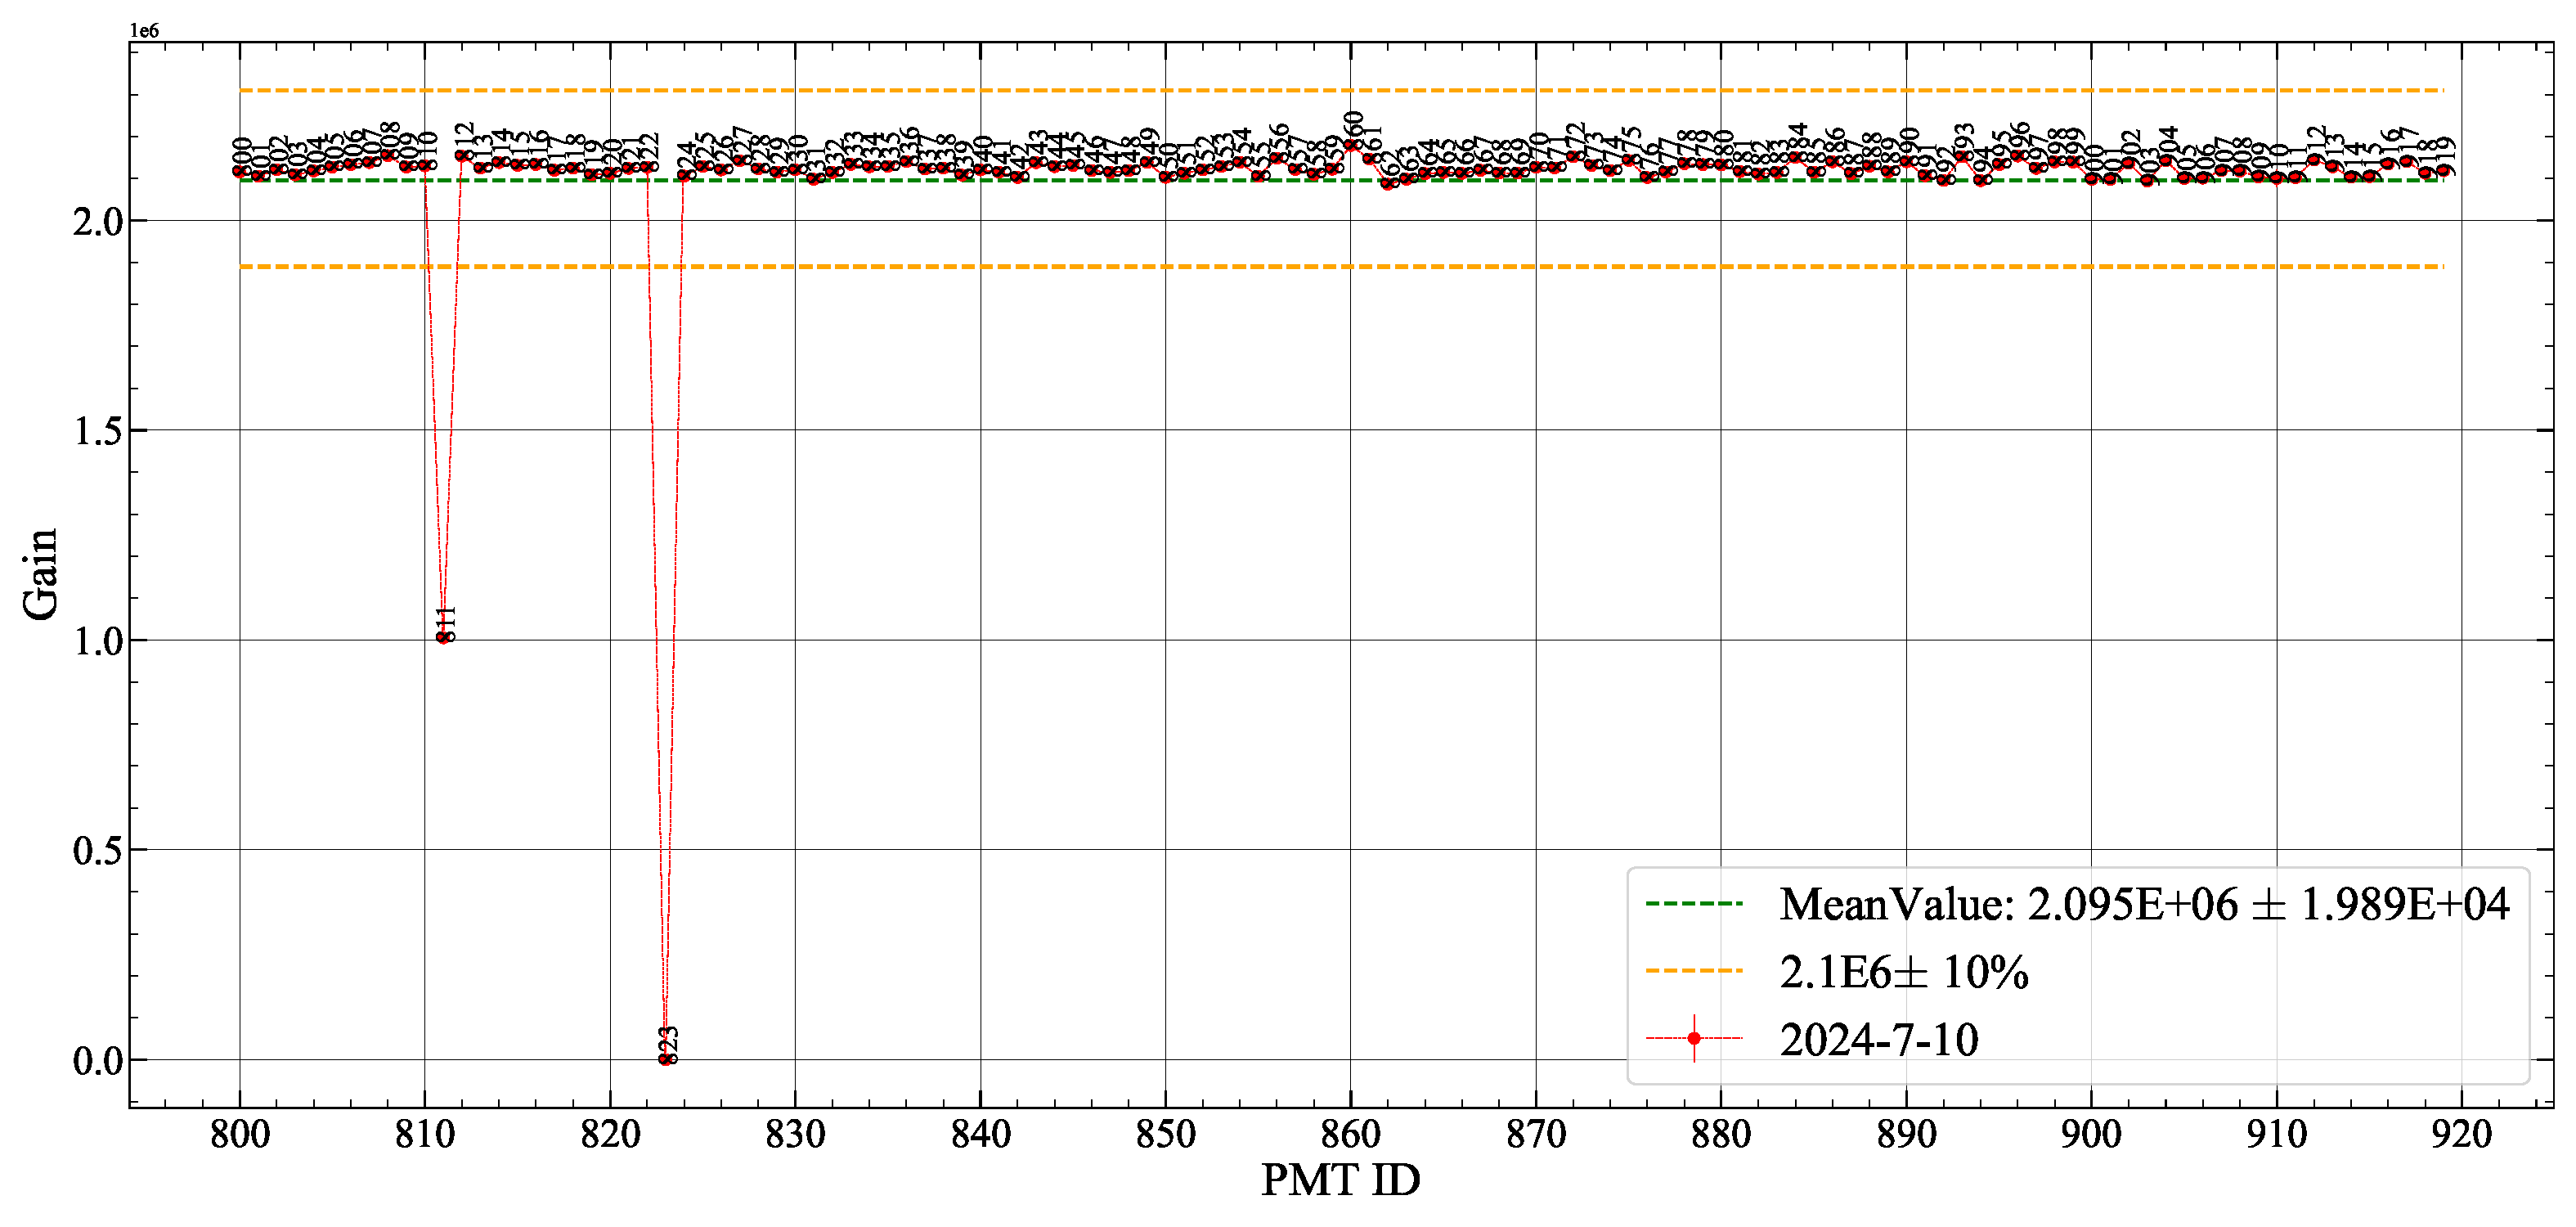
\includegraphics[width=\textwidth]{figures/ODCommissioning/2024-7-10_ODPMT_Gain.pdf}
    \caption{A scatter plot of the OD PMT Gain versus PMT ID for each OD PMT from a measurement taken on July 10th 20254.}
    \label{fig:ODPMTGain_2024-7-10}
\end{sidewaysfigure}

\subsection{Monitoring PMT Response Over Time}
Whilst operating the PMTs it is important to monitoring their response as the SPhE Area size and gain can drift over time \cite{DayaBay:2016ggj,Super-Kamiokande:2023jbt}. Using the data collected during the monthly OD SPhE measurements, the distribution of gain and SPhE size was tracked throughout the WS2022 and WS2024 science runs (until the time of writing) with gain versus PMT ID scatter plots as shown in \autoref{fig:RelativeGain_WS2022} and \autoref{fig:RelativeGain_WS2024}.
To monitor the observed $<1\%$ change in gain month-by-month, the relative change with respect to the start of each science run was measured. During the WS2022 science run, a mean relative change of PMT gain was measured to $(0.81\pm0.47)\%$. At the time of writing, a mean relative change of PMT gain of $(1.37\pm0.25)\%$ was measured for the WS2024 science run. Whilst the average gain change across all PMTs is relatively small, it can be seen in \autoref{fig:RelativeGain_WS2024} that individual PMTs drift at different rates. Due to the short run length of WS2022 it was not necessary to adjust the PMTs voltages to gain match across the PMT array during the science run, however there was a gain matching campaign in May 2022 following the science run. Prior to the start of the WS2024 science run, the OD PMTs were gain matched again to $2.1\times10^{6}$. After 15 months of operation it was necessary to perform another gain match of the OD PMTs as PMT 859 had a relative change in gain $>10\%$ with other PMTs also approaching the $10\%$ limit set by LZ.

\begin{sidewaysfigure}[ht!]
    \centering
    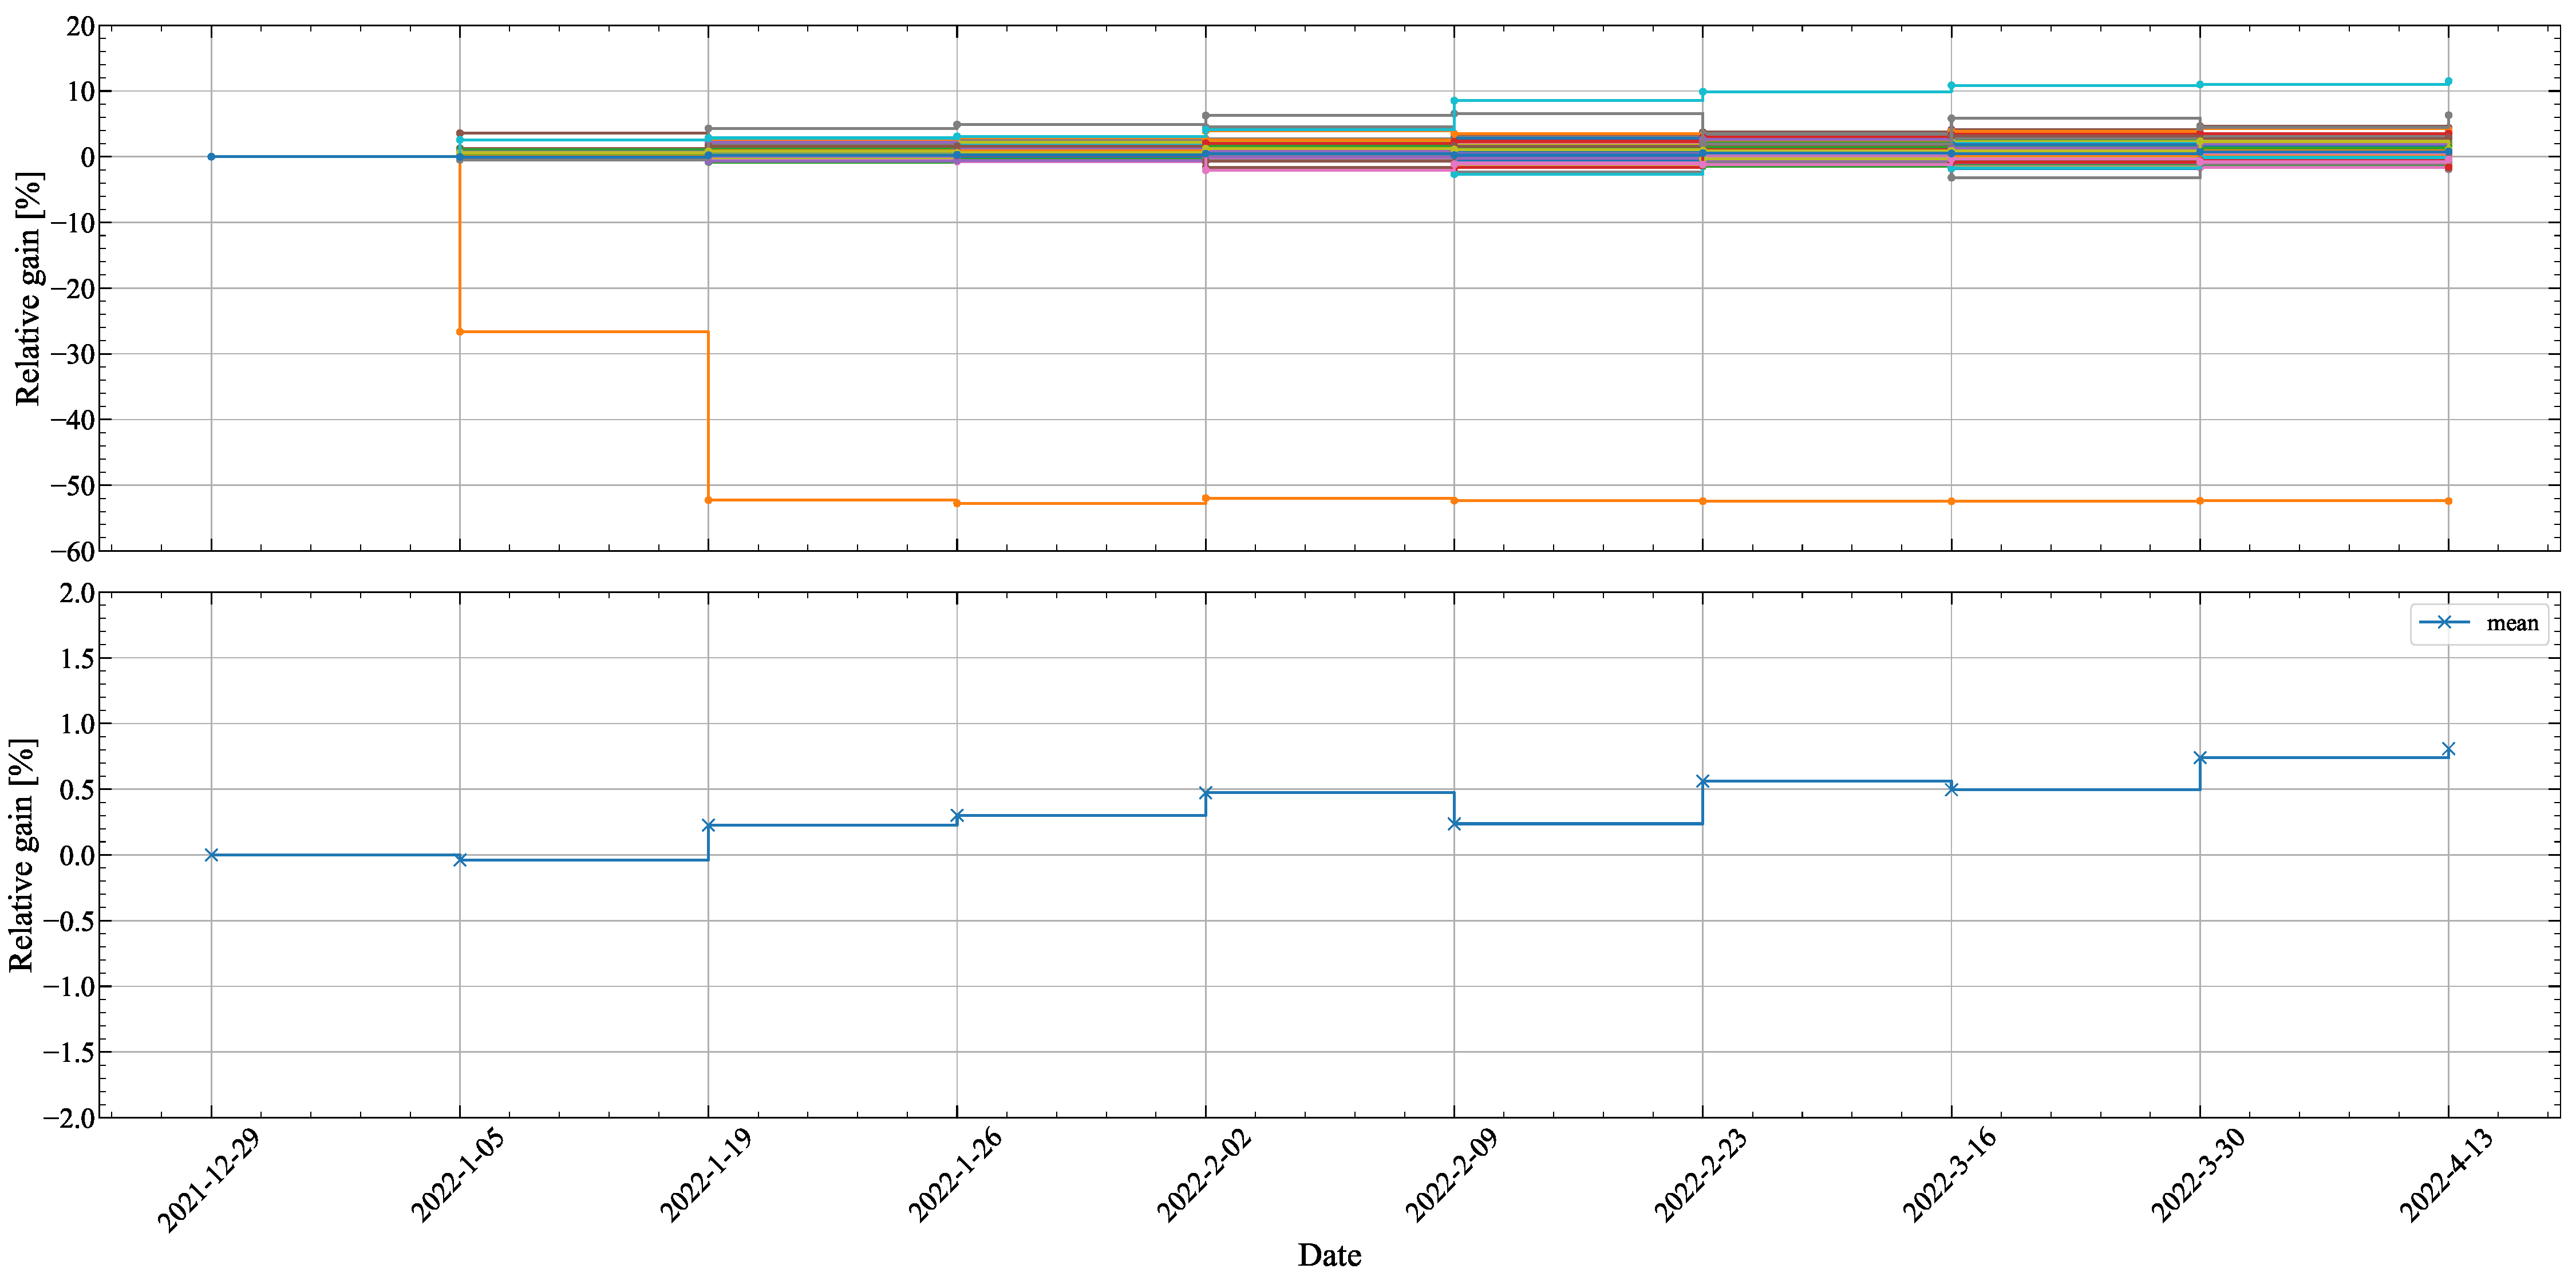
\includegraphics[width=\textwidth]{figures/ODCommissioning/RelativegainOverTime_AllPMTs_Both_Full_WS2022.pdf}
    \caption{\textbf{Top:} A scatter plot of the relative change in OD PMT Gain over WS2022 science run. The reduced gain of PMT 811 can be seen in orange. \textbf{Bottom:} A scatter plot of the average relative change in OD PMT Gain across all OD PMTs over WS2022 science run.}
    \label{fig:RelativeGain_WS2022}
\end{sidewaysfigure}
\begin{sidewaysfigure}[ht!]
    \centering
    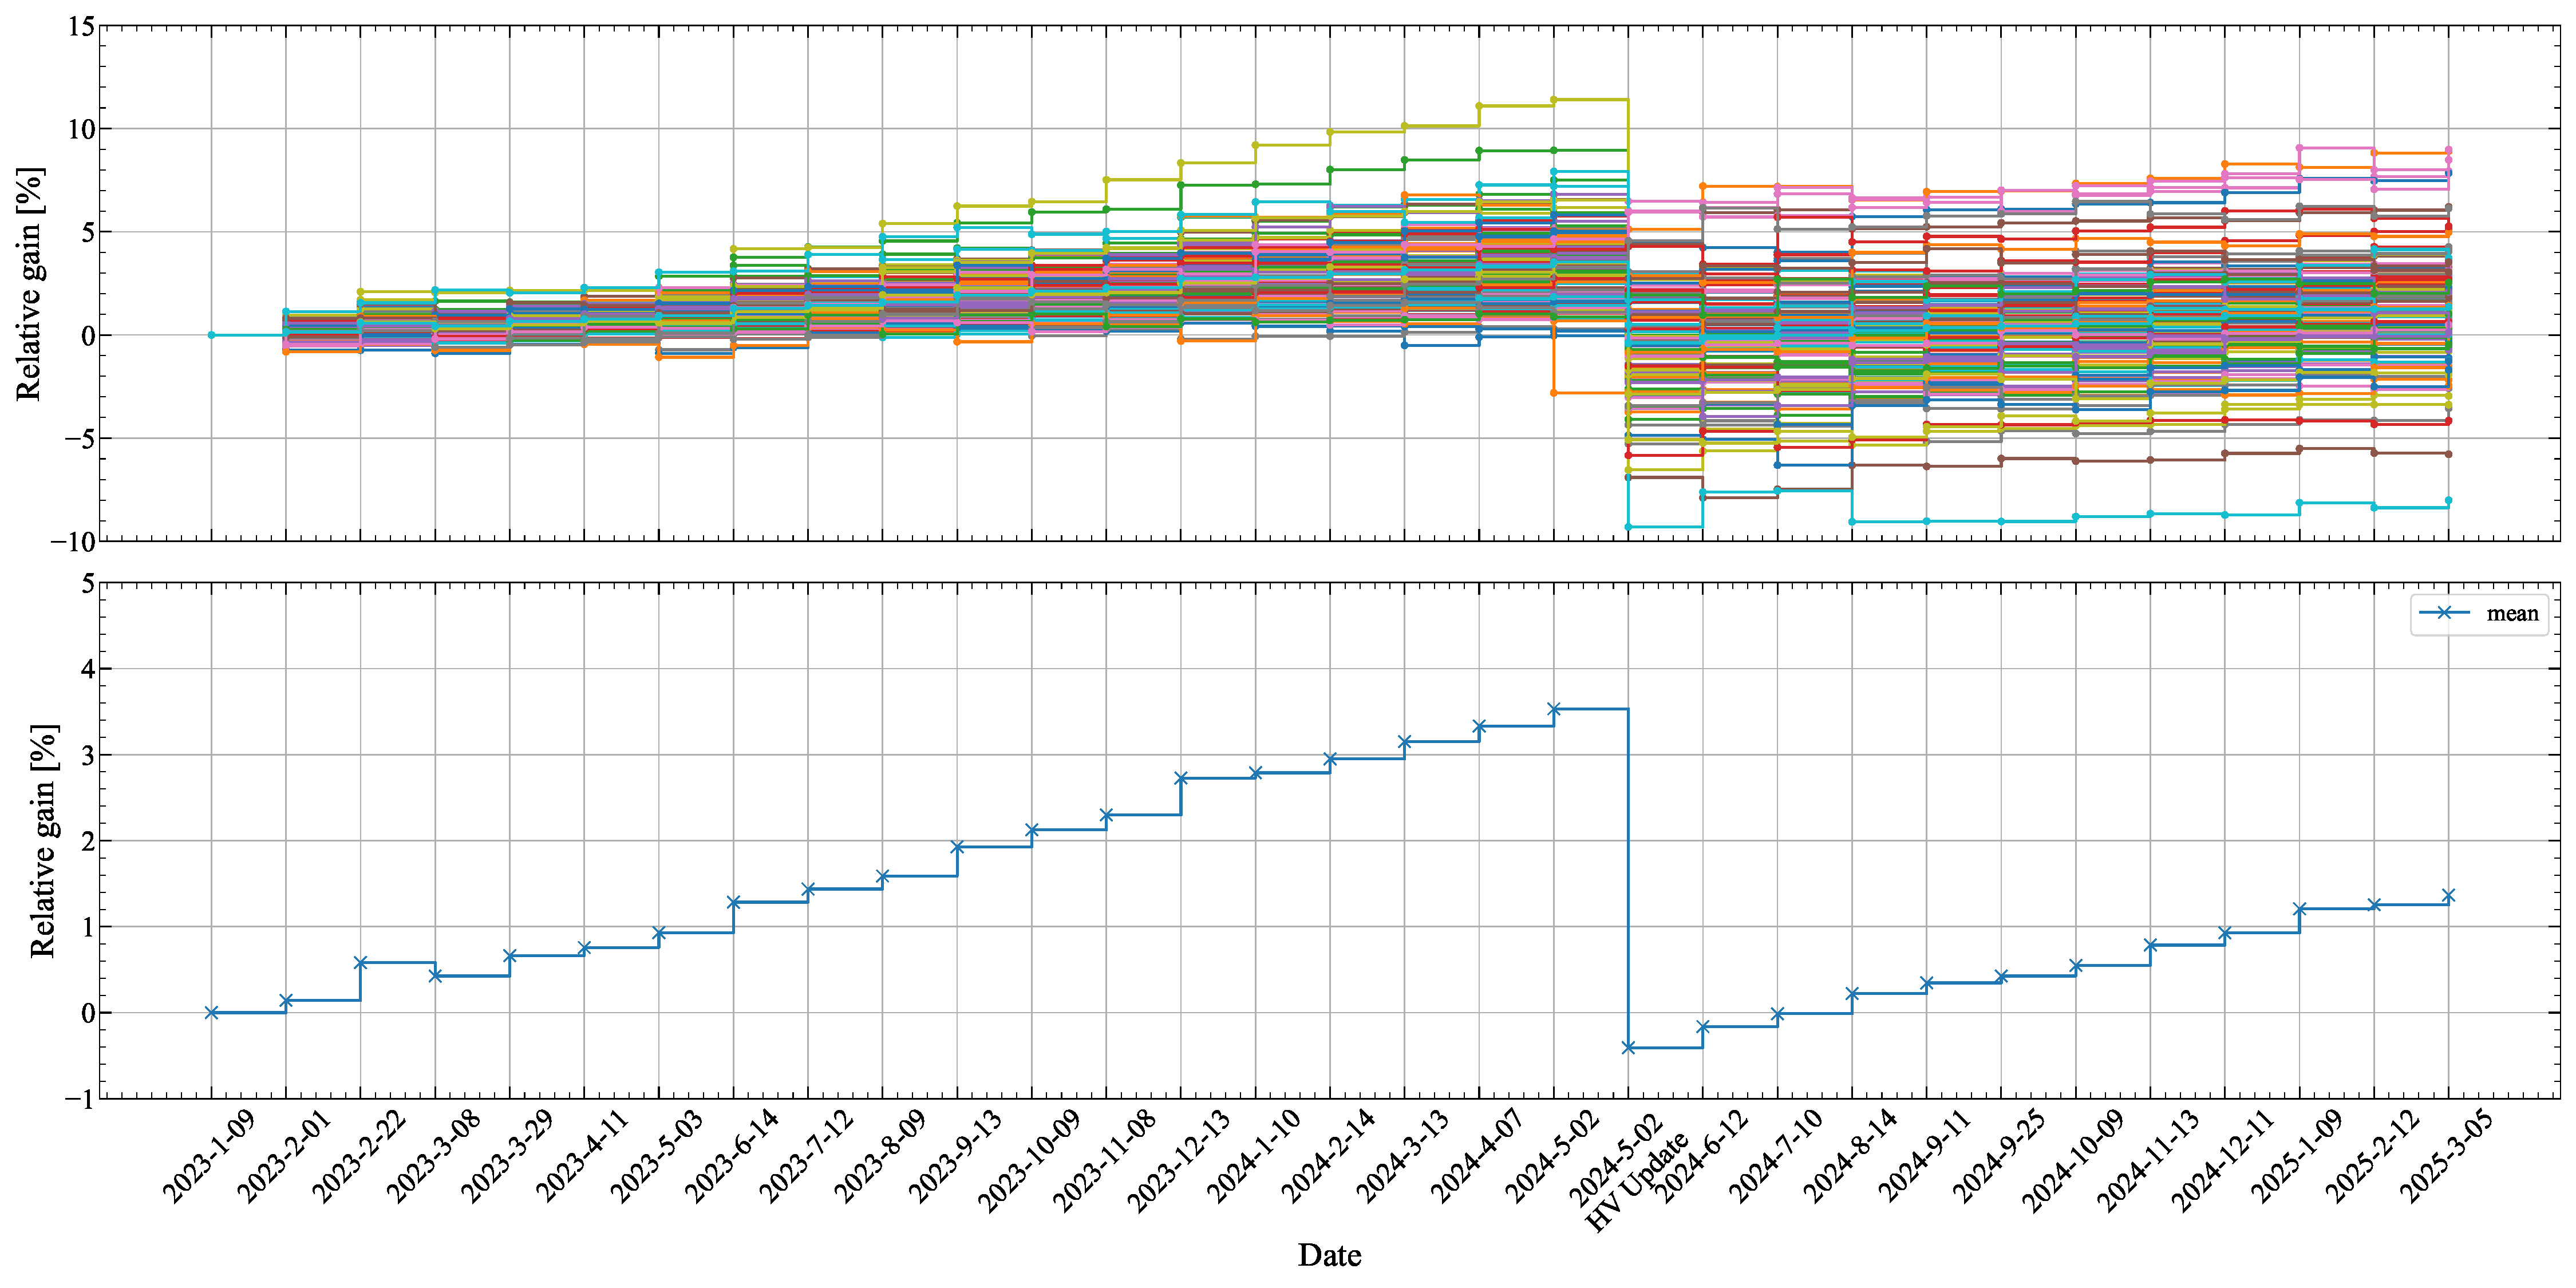
\includegraphics[width=\textwidth]{figures/ODCommissioning/RelativegainOverTime_AllPMTs_Both_Full_WS2024.pdf}
    \caption{\textbf{Top:} A scatter plot of the relative change in OD PMT Gain since the start of the WS2024 science run (until the time of writing). \textbf{Bottom:} A scatter plot of the average relative change in OD PMT Gain across all OD PMTs since the start of the WS2024 science run (until the time of writing).}
    \label{fig:RelativeGain_WS2024}
\end{sidewaysfigure}
\begin{sidewaysfigure}[ht!]
    \centering
    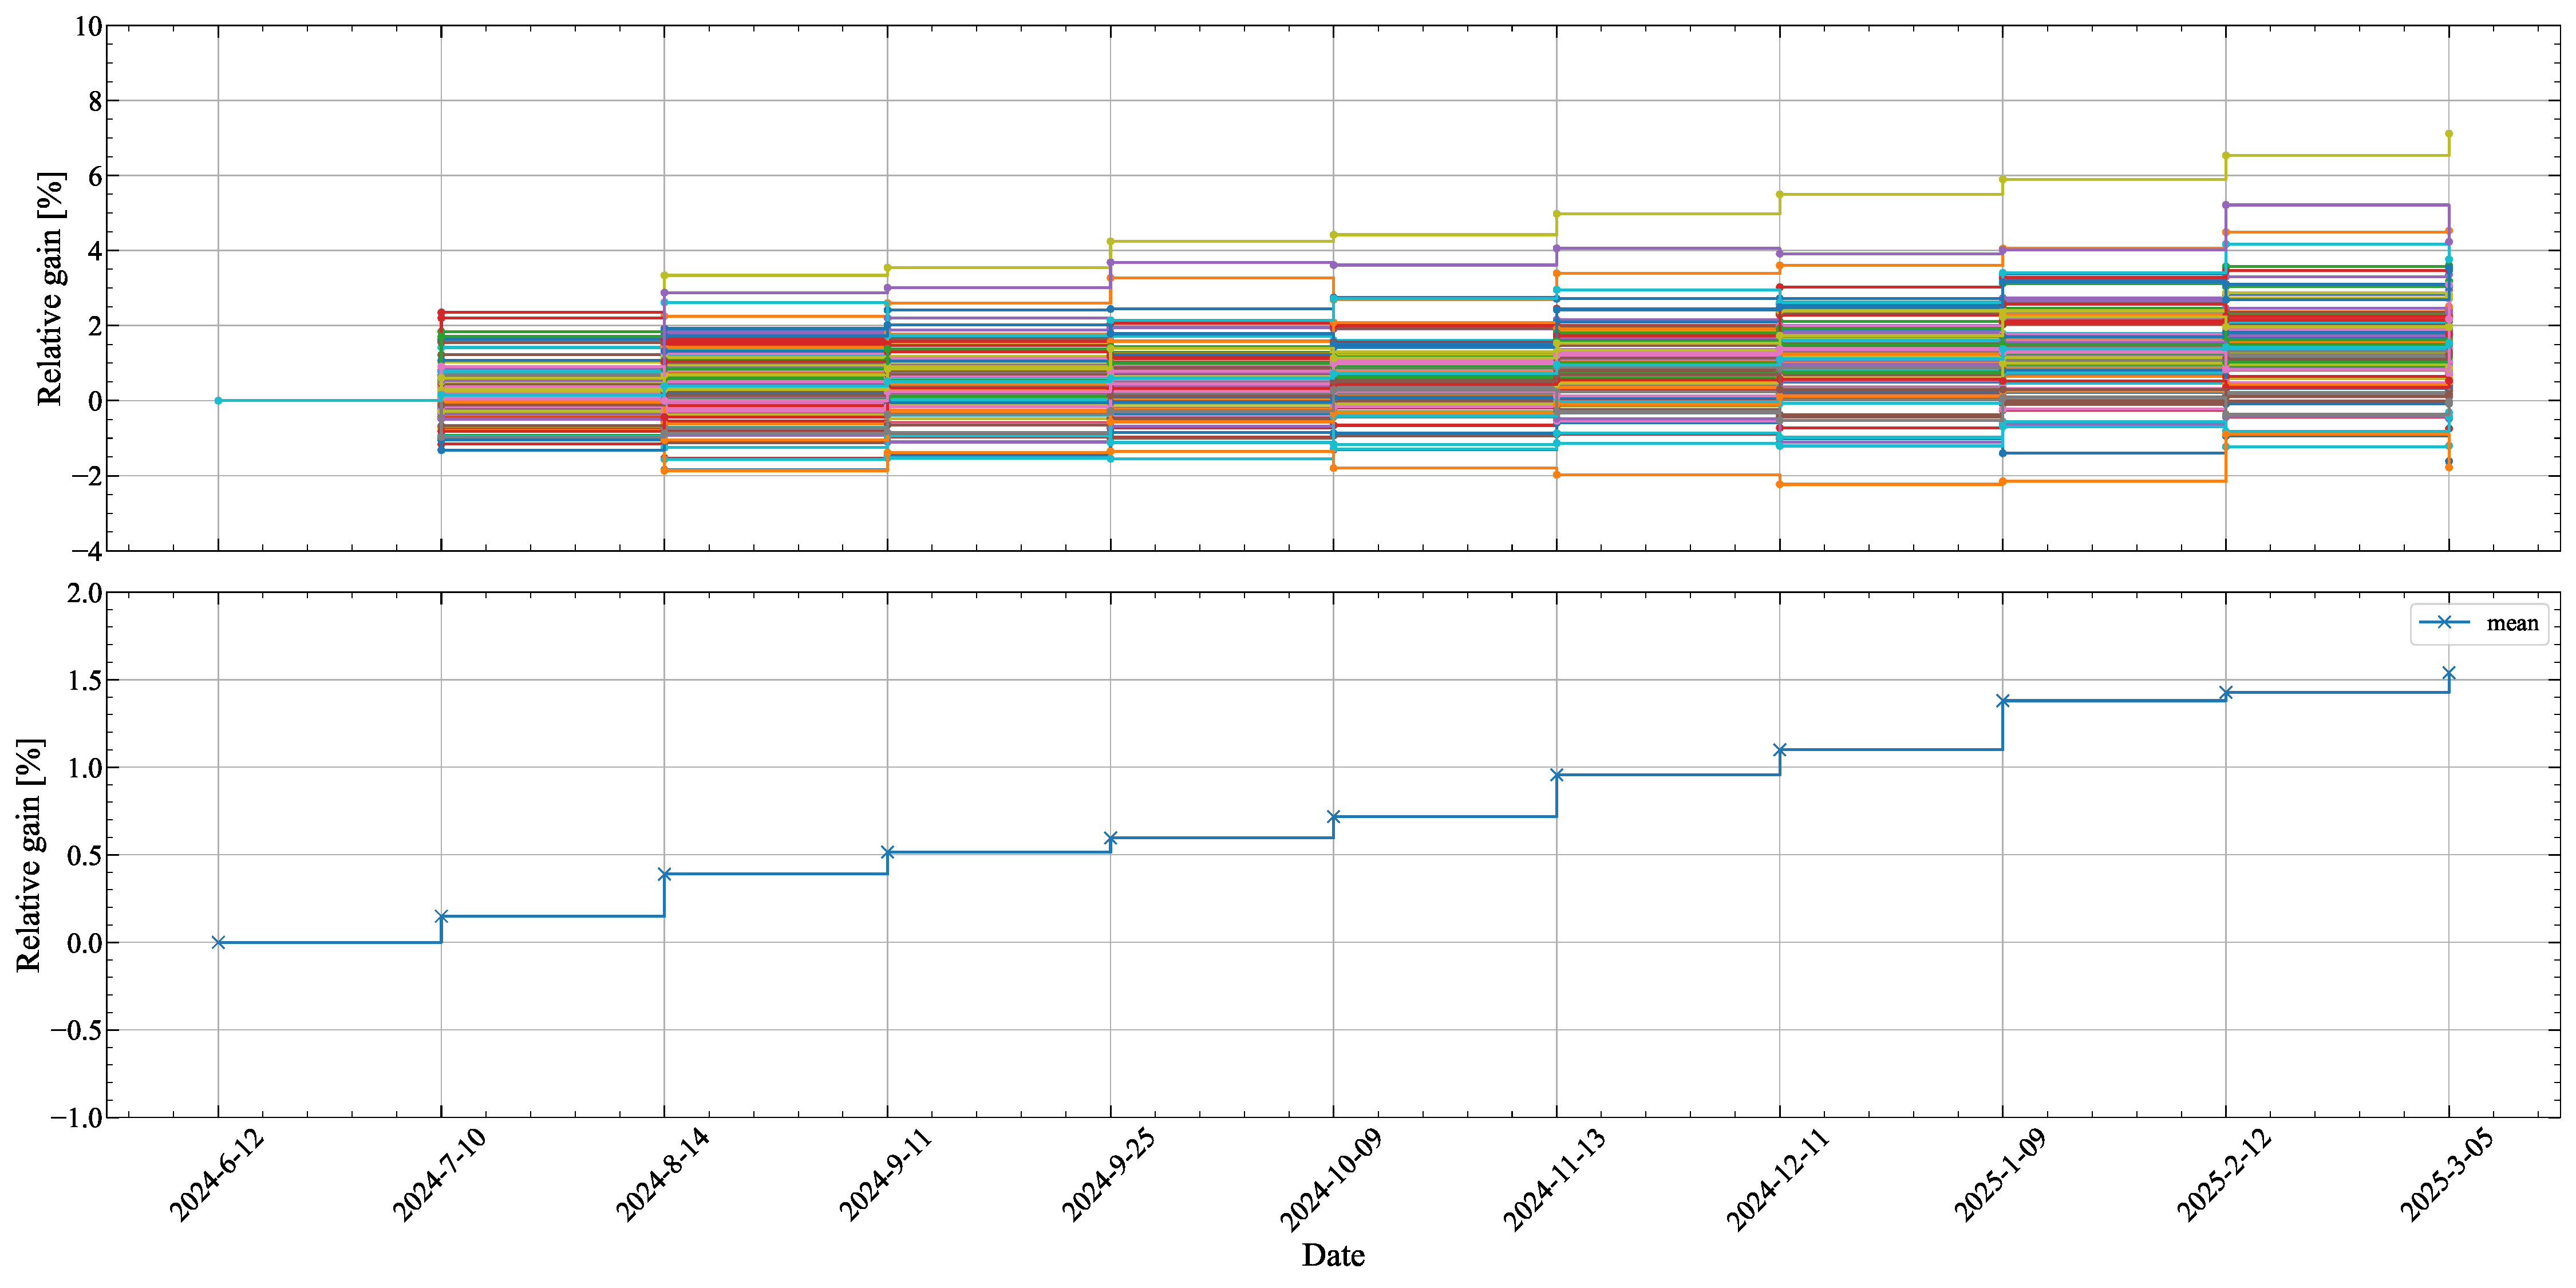
\includegraphics[width=\textwidth]{figures/ODCommissioning/RelativegainOverTime_AllPMTs_Both_Full_WS2024May2024Onwards.pdf}
    \caption{\textbf{Top:} A scatter plot of the relative change in OD PMT Gain since the gain matching campaign in May 2024 (until the time of writing). \textbf{Bottom:} A scatter plot of the average relative change in OD PMT Gain across all OD PMTs since the gain matching campaign in May 2024 (until the time of writing).}
    \label{fig:RelativeGain_WS2024May2024Onwards}
\end{sidewaysfigure}
\subsection{Gain Curves}
\section{Trigger Efficiency}

\section{Optical Calibration System Development}
\subsection{UV LED commissioning}

\subsection{Monitoring PMT}
\chapter{Veto efficiency studies for the 2024 WIMP search analysis}\label{chap:VetoEfficiency}
A WIMP scatter is expected to only deposit a small amount of energy (few~keV) within the LXe volume of the experiment in a single scatter. 
Neutrons produced through radioactive decays within detector materials mimic a WIMP interaction when they scatter off Xe atoms. Veto detectors surrounding the central LXe volume can detect these otherwise indistinguishable events and also permit the assessment of the local radioactivity environment. A WIMP discovery will require an excellent understanding of all background sources, which is best done through the characterization of those backgrounds \textit{in situ}. The efficiency of the veto systems in the detection of the radiation produced by the backgrounds should be maximised whilst minimizing the impact of the veto selection on detector livetime, in turn maximising the detector livetime available for the detection of WIMPs. \autoref{sec:VetoEff/simulation_improvements} describes the series of improvements to the detector simulation geometry that were made before the WS2024 science run, which aided the understanding of the response from the veto detector systems. The refinement of the veto selection algorithm is discussed alongside the impact that the veto selection had on the WS2024 result from \autoref{sec:VetoEff/VetoSelectionOptimisation} onwards.

\section{Improved Outer Detector Simulations}\label{sec:VetoEff/simulation_improvements}
The Outer Detector is defined as a Geant4 geometry, including transparency and other properties of each material, to allow simulations of neutron vetoes. 
Before the WS2024 result, there were a number of major differences between simulations and data in the Outer Detector (OD). As such, an effort was made to correct this through modifications to the geometry of the Outer Detector in simulations to better reflect what is observed in data.

\subsection{Modifications of the Outer Detector simulation geometry}\label{sec:VetoEff/GeometryEdits}
There was a distinct discrepancy in neutron capture timing following single scatters within the TPC. This was one of the metrics that was investigated to quantify the difference between data and simulation. This discrepancy is shown in \autoref{fig:VetoEff/NC_AmLi_50mm7} through the comparison between what is measured in data and the ``baseline simulation''.
The simulation is improved through the following changes:
\begin{enumerate}
	%\item Spacing was added between the acrylic tanks to account for the gaps between the tanks which were present due to minor geometric differences produces in the moulding of the vessels during manufacturing process.
	\item Water was added to the foam volume, which is between the OCV and acrylic tanks. The foam was intended to displace water to reduce neutron capture time; however, the foam became saturated with water.
    
	\item The acrylic tanks were moved further away from the OCV in the simulation to reflect the actual position of the tanks in the Outer Detector, as installed.
\end{enumerate}
A series of simulations is produced varying both the amount of water saturation of the foam displacer in 1\% steps and the position of the acrylic tanks from the OCV in 10~mm steps. A photograph of the foam displacer that encases the OCV is shown in \autoref{fig:VetoEff/od_geometry_for_sr3}, alongside a cross-section of the BACCARAT output geometry.

\begin{figure}[h!]
	\centering
	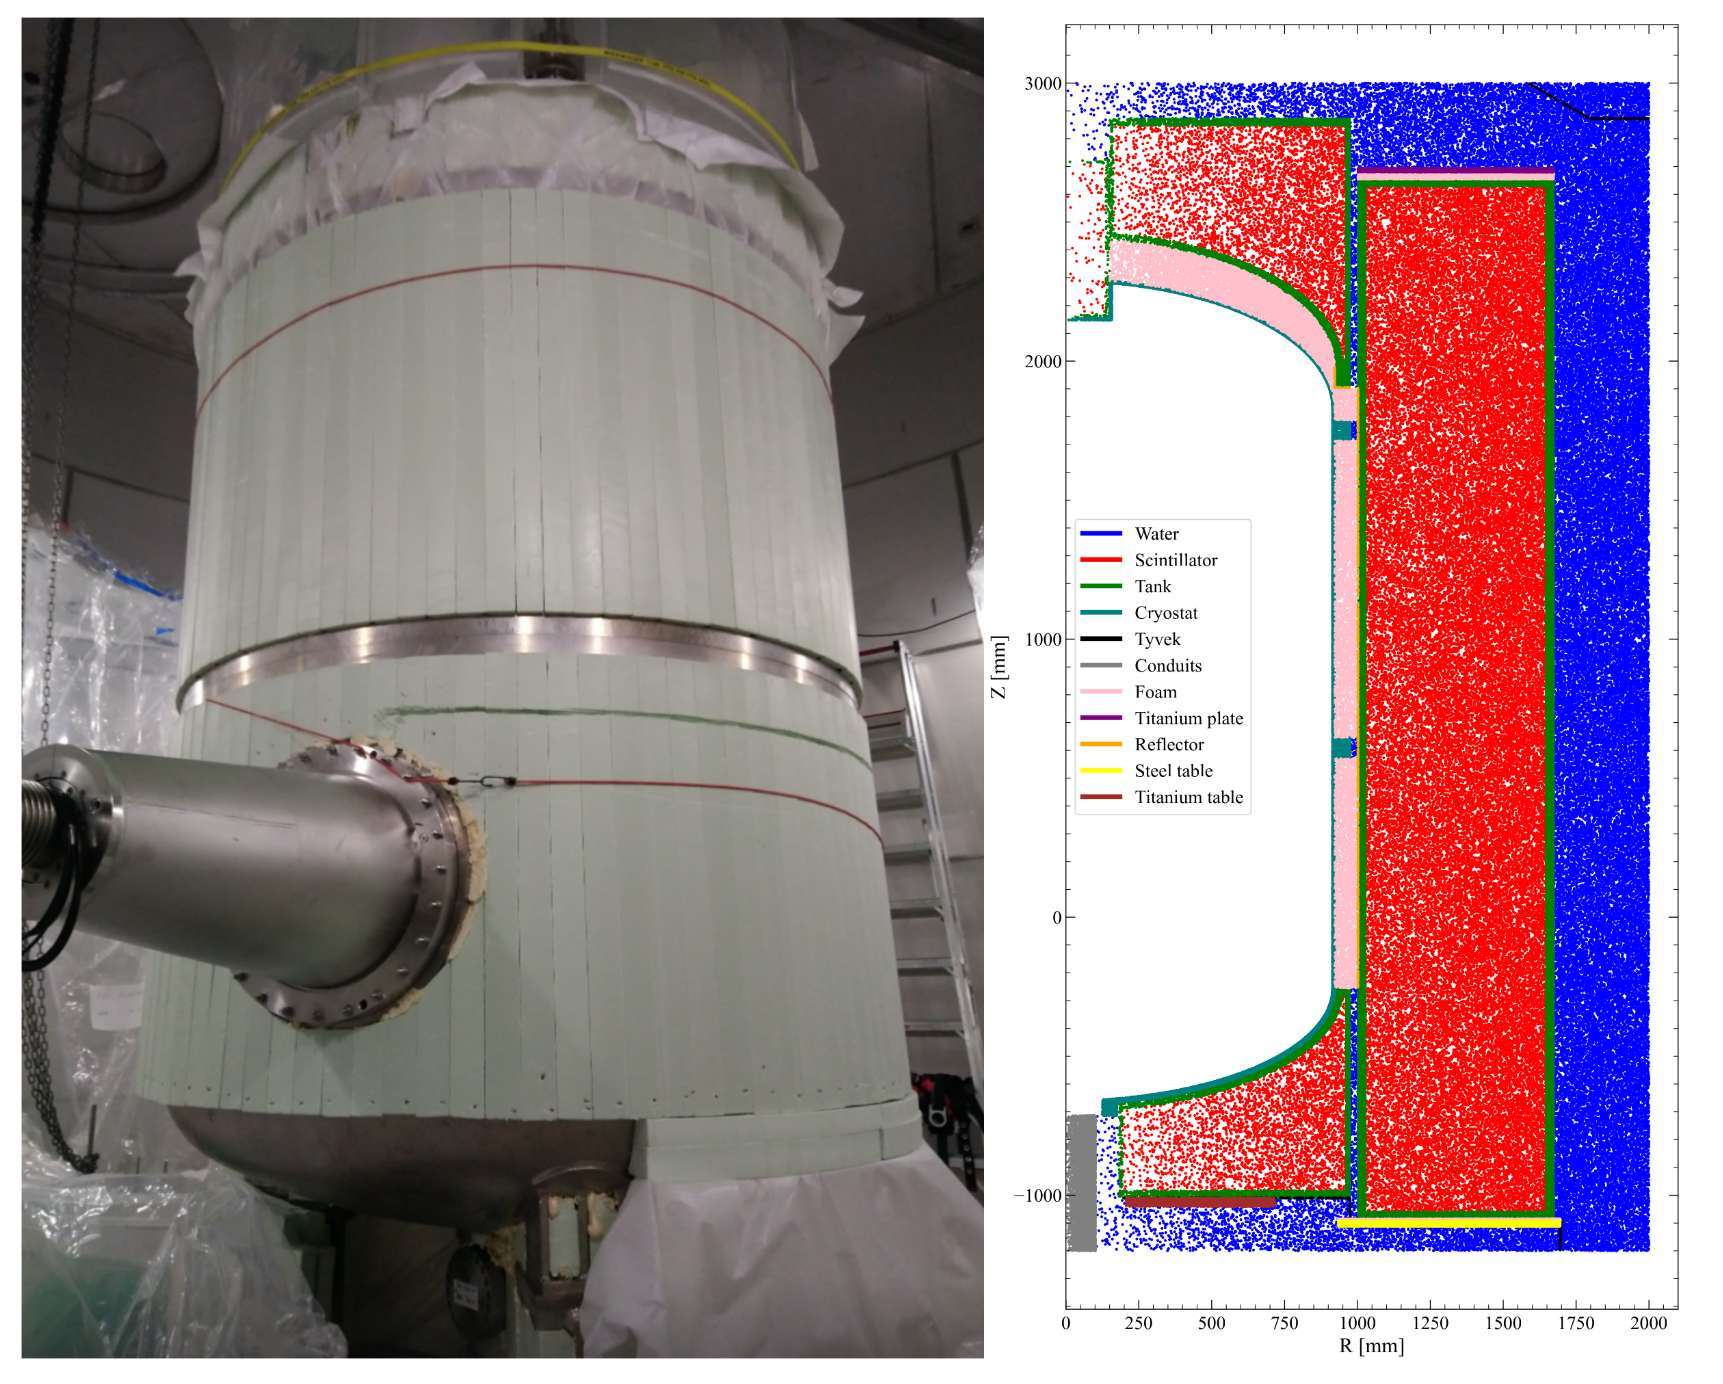
\includegraphics[width=0.8\textwidth]{figures/VetoEfficiency/FoamImgAndSimGeoTogether.png}
	\caption[An image of the foam displacer surrounding the OCS and final geometry in the simulation used for the WS2024 science run.]{Geometry in the simulation used for the WS2024 science run. \textbf{Left:} A photograph of the light green foam water displacer, which resides between the acrylic tanks and the OCV. The water displacer was wrapped in a light reflector made from Tyvek. \textbf{Right:} A cross-section of the BACCARAT output. Geantinos (non-interacting test particles used for visualisation) were passed through the simulation geometry, and the $xyz$ position information and Geant4 volumes were recorded to show the various volumes in the simulation.}
	\label{fig:VetoEff/od_geometry_for_sr3}
\end{figure}

Following these geometry changes, the neutron capture timing using AmLi is studied. Events which are classified as single scatters by LZap and pass the selection outlined in \autoref{sec:app/WSCoreCuts} are used for the study. OD pulses which exceeded a 200~keV (49~phd) threshold are used to optimise the geometry as this corresponds to the threshold associated with proton recoil of neutrons of hydrogen in the OD medium.
All possible configurations of the geometry modifications are visually examined to determine which variation of simulation matches the data. An example of the comparison plot is shown in \autoref{fig:VetoEff/NC_AmLi_50mm7}; the "baseline simulation" is the initial configuration of the geometry before this study.
From this study, it was found that 30~mm~to~50~mm movement of the SATs alongside 5\%~to~7\% increase in the percentage of water in the foam provides the best agreement between data and simulation at a 200~keV threshold. Including results from other studies on the H-Gd neutron capture ratios, where more water is present and thus more hydrogen, the \textit{best} configuration of the simulation geometry changes is found to be 30~mm and 6\% through matching the capture time of neutrons following single scatters in the active LXe volume.
\begin{figure}[!h]
	\centering
	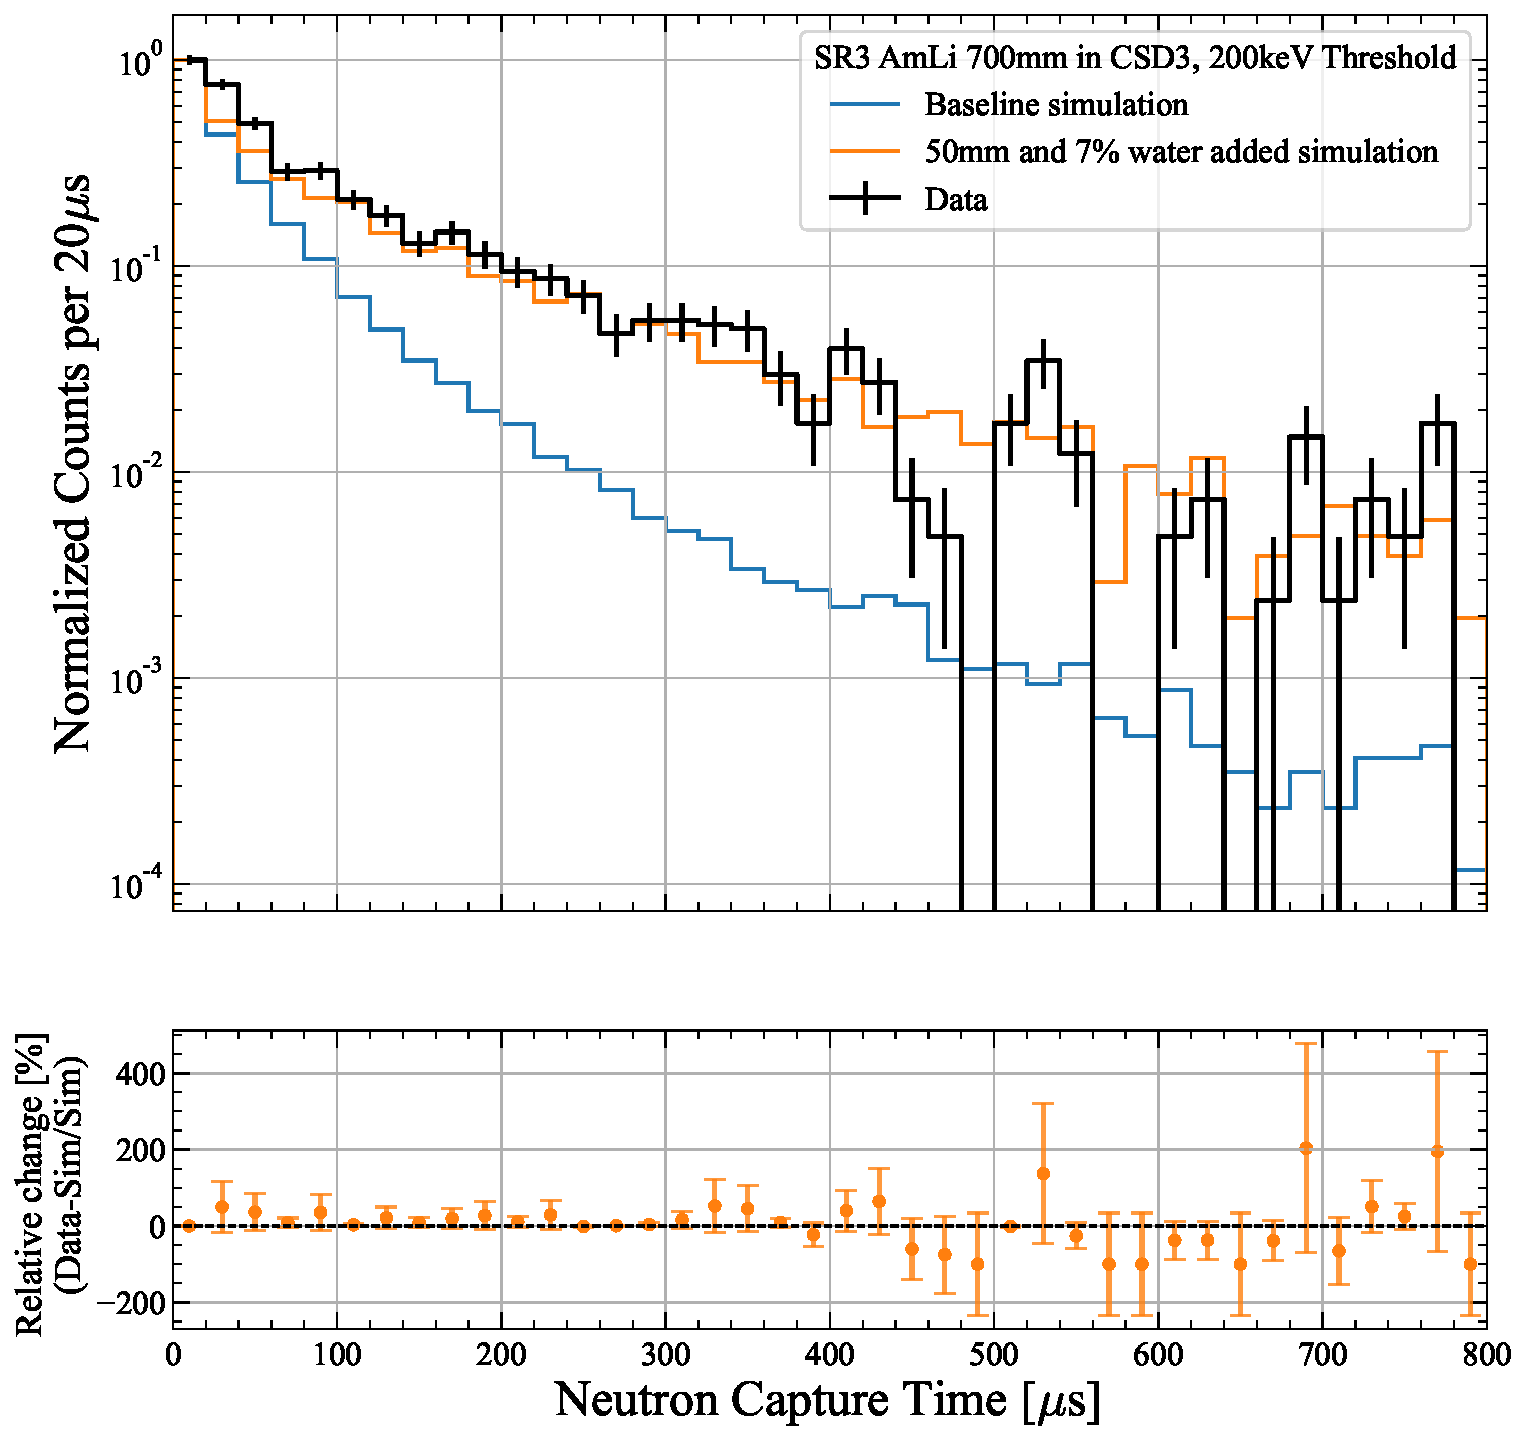
\includegraphics[width=0.8\linewidth]{figures/VetoEfficiency/movedSAT50mm_7percentWater_AmLi_CSD3_Z700mm_200keV_Ratio.pdf}
	\caption[An example of the plot used to compare neutron capture timing in data with the baseline simulation and the modified simulation.]{An example of the plot used to compare neutron capture timing in data with the baseline simulation and the modified simulation. The relative change between data and simulation in each $20~\mu s$ bin is used to aid the visually examination across a 1200~\textmu s window.}
	\label{fig:VetoEff/NC_AmLi_50mm7}
\end{figure}

\section{Veto selection optimisation}\label{sec:VetoEff/VetoSelectionOptimisation}
A description of how the veto selection for the WS2024 is optimised is presented in this section. The Skin and OD veto cuts used in the WS2024 science run are based on those developed for the WS2022 science run, described in Ref.~\cite{LZ:2022lsv}, and are presented in \autoref{tab:VetoEff/sr3_veto_cuts}.
Both the OD and Skin detector may issue a veto, and for each detector, a tighter selection is defined for the first period after an interaction (\textit{prompt}) while a looser selection is applied for a longer time interval (\textit{delayed}), giving four veto categories each with their own intended purpose:
\begin{itemize}
	\item \textit{Skin-prompt} used for tagging $\gamma$-rays in the Skin detector
	\item \textit{OD-prompt} used for tagging $\gamma$-rays and neutron proton recoils in the OD
	\item \textit{Skin-delayed} used for tagging $\gamma$-rays from post-neutron capture de-excitation
	\item \textit{OD-delayed} used for tagging $\gamma$-rays from post-neutron capture de-excitation
\end{itemize}
The cuts used for the different veto criteria are selected at the same time as the AmLi neutron tagging efficiency calculation, and are optimised to maximise the tagging efficiency whilst reducing deadtime. \textit{Pulse area} threshold, \textit{PMT coincidence} threshold, and \textit{veto window length} are the three different variables that can be tuned for this optimisation. Events which were classified as single scatters by LZap and pass the selection outlined in \autoref{tab:VetoEff/amli_efficiency_cuts} are used for the study. The following subsections describe how each of the veto selection variables is tuned.

\begin{table}[!ht]
	\centering
	\caption[Outline of TPC cuts applied to AmLi calibration data for determining the veto efficiency.]{Outline of TPC cuts applied to AmLi calibration data for determining the veto efficiency. All cuts are defined in \autoref{sec:app/WSCoreCuts}.}
	\label{tab:VetoEff/amli_efficiency_cuts}
    \scalebox{0.9}{
	\begin{tabular}{llll}
    \hline\hline
    \textbf{Livetime cuts}&\textbf{Physics cuts}& \textbf{S2 cuts}& \textbf{S1 cuts}\\
    \hline
    Burst noise cut& Single scatter& S2 width vs drift time& S1 Stinger \\
    Muon holdoff& S1 threshold & Narrow S2& S1 TBA vs drift time\\
    Bad buffer cuts& S2 threshold& S2 rise time& S1 HSC \\
    Excess Area cut& Fiducial Volume& S2 early peak& S1 Shape\\
    & & S2 XY quality&\\
    & & S2 TBA &\\
    \hline\hline
	\end{tabular}}
\end{table}

\subsection{Veto window length}\label{sec:VetoEff/VetoWindowLength}
The veto window length is defined as the period of time after a single scatter in the TPC where a coincident signal in the OD or Skin would cause the event.
The veto window length for the prompt windows is determined using AmLi and DD calibration data by measuring the time difference between the TPC single-scatter and OD and Skin pulses. The length of the prompt window is determined by the width of the peak observed in the pulse timing distributions shown in \autoref{fig:VetoEff/veto_prompt_windows}. For the WS2024 selection, no change is made to the OD prompt veto window size; however, the Skin prompt veto window is reduced by 500~ns as the pulses observed outside of the window $(0-250)$~ns are large enough to be rejected by the subsequent delayed veto, and there are no pulses observed before $-250$~ns.
\begin{figure}[!ht]
	\centering
	\begin{subfigure}[b]{0.49\textwidth}
		\centering
		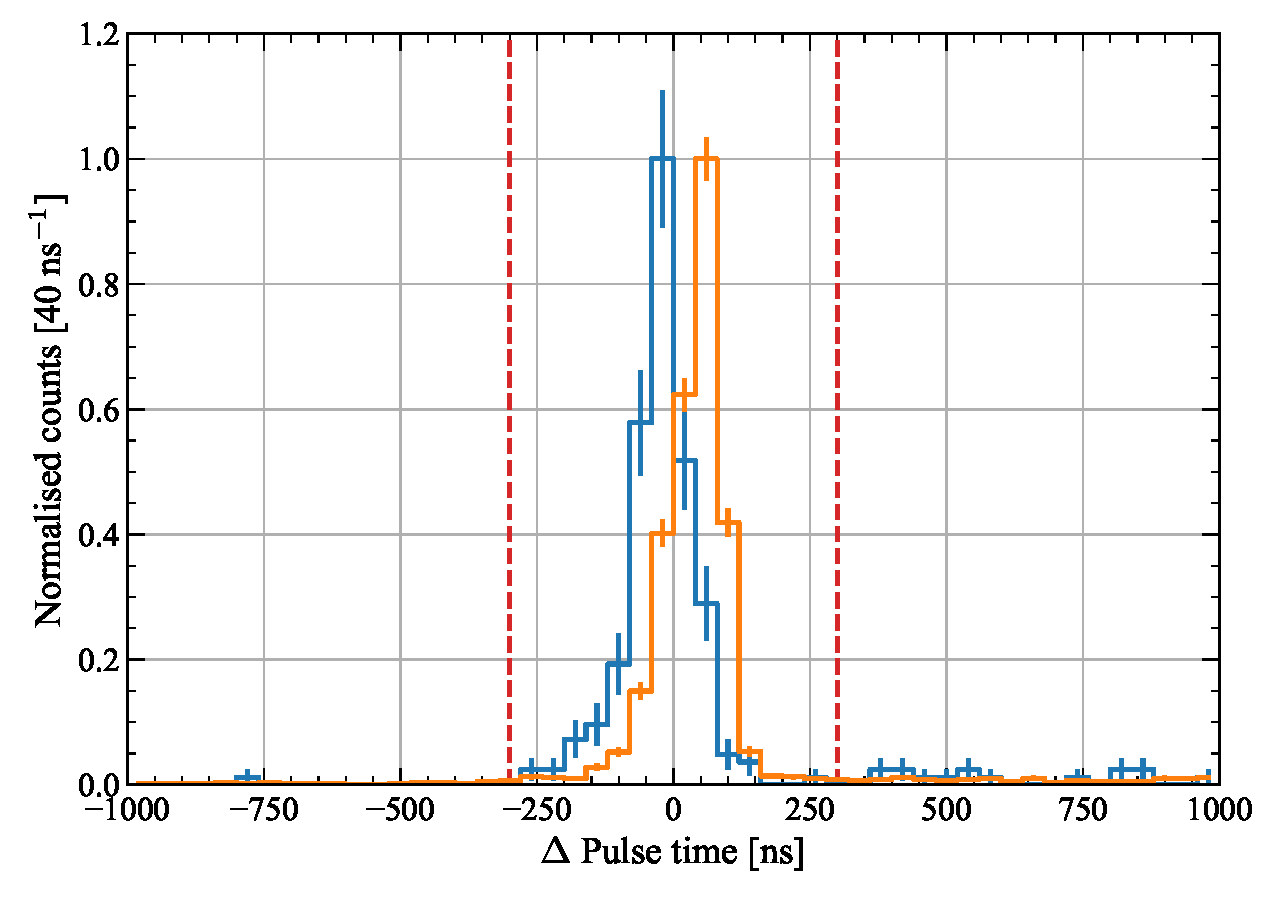
\includegraphics[width=\textwidth]{figures/VetoEfficiency/ODpromptWindowTiming.pdf}
		%\caption{Time difference (in ns) between TPC single-scatter and OD pulses using AmLi data.}
        \caption{}
		\label{fig:VetoEff/od_prompt_window}
	\end{subfigure}
	\hfill
	\begin{subfigure}[b]{0.49\textwidth}
		\centering
		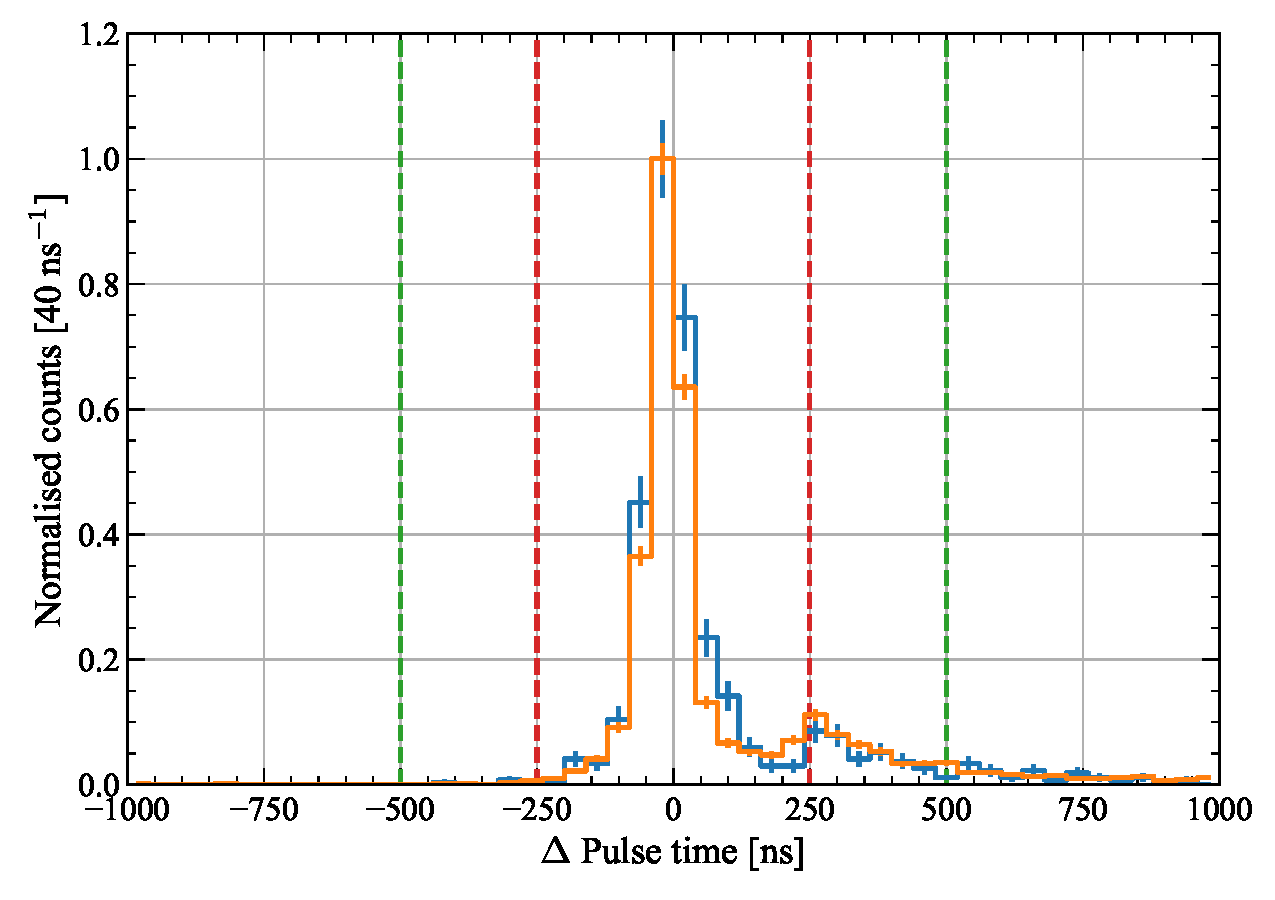
\includegraphics[width=\textwidth]{figures/VetoEfficiency/SkinpromptWindowTiming.pdf}
		%\caption{Time difference (in ns) between TPC single-scatter and OD pulses using DD data.}
		\caption{}
        \label{fig:VetoEff/skin_prompt_window}
	\end{subfigure}
	\caption[Prompt timing window for the OD (left) and Skin (right). 
    AmLi (blue) and DD (orange) calibration data was used to measure the time difference between the TPC single scatter pulse and veto pulse.]{Prompt timing window for the OD (left) and Skin (right). 
    AmLi (blue) and DD (orange) calibration data was used to measure the time difference between the TPC single scatter pulse and veto pulse. 
    The vertical red lines indicate the boundary of the timing selection used for WS2024. There is no change in the size of the OD prompt veto window whereas the Skin prompt veto window is reduced by a total of 500~ns. The WS2022 veto window limits are shown in green.}
	\label{fig:VetoEff/veto_prompt_windows}
\end{figure}

The veto efficiency (defined in \autoref{eqn:VetoEff/neutron_tagging_efficiency}) calculated using AmLi calibration data is used to determine the size of the delayed veto window for both the Skin and OD. The veto window length is reduced by a factor of two for both Skin and OD delayed windows as the slope of the efficiency curve begins to plateau above 600~\textmu s. An example of the veto efficiency plot used is shown in \autoref{fig:VetoEff/DelayedVetoWindow}.
\begin{figure}[!ht]
    \centering
    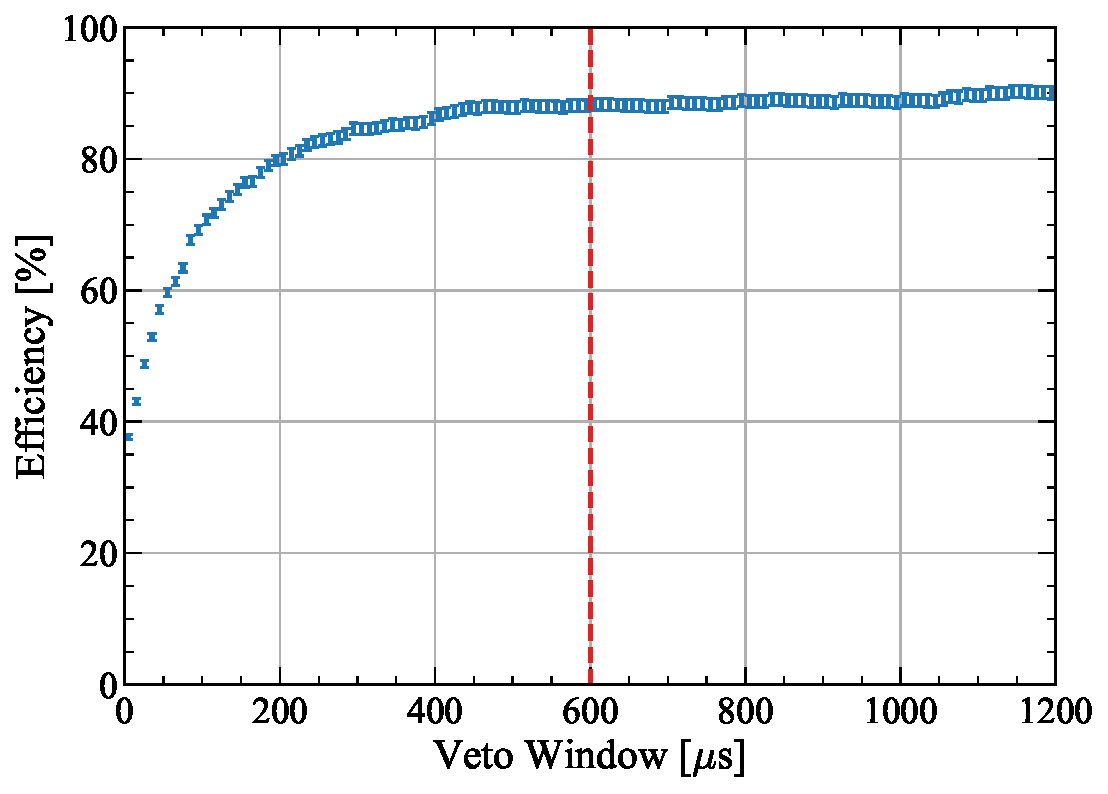
\includegraphics[width=0.7\linewidth]{figures/VetoEfficiency/DelayedVetoWindow.pdf}
    \caption[An example of a veto efficiency curve measured using AmLi calibration data.]{An example of a veto efficiency curve measured using AmLi calibration data. The vertical red line indicates the WS2024 upper bound of the delayed veto windows used for both the Skin and OD.}
    \label{fig:VetoEff/DelayedVetoWindow}
\end{figure}

The reduction in the veto window lengths has a positive impact on the dead time induced by the veto selection. Veto dead time is discussed in greater detail \autoref{sec:VetoEff/DeadtimeStability}.

\subsection{PMT Coincidence and pulse area threshold}
To optimize the pulse area and PMT coincidence thresholds the veto efficiency and deadtime are calculated for a grid in the pulse area and PMT coincidence requirement for the respective veto windows. An example of an efficiency grid (``heatmap'') is shown in \autoref{fig:VetoEff/od_prompt_veto_heatmap}. The efficiency of the veto increases with decreasing pulse area and PMT coincidence threshold, whereas deadtime follows the opposite trend.

\begin{figure}
	\centering
	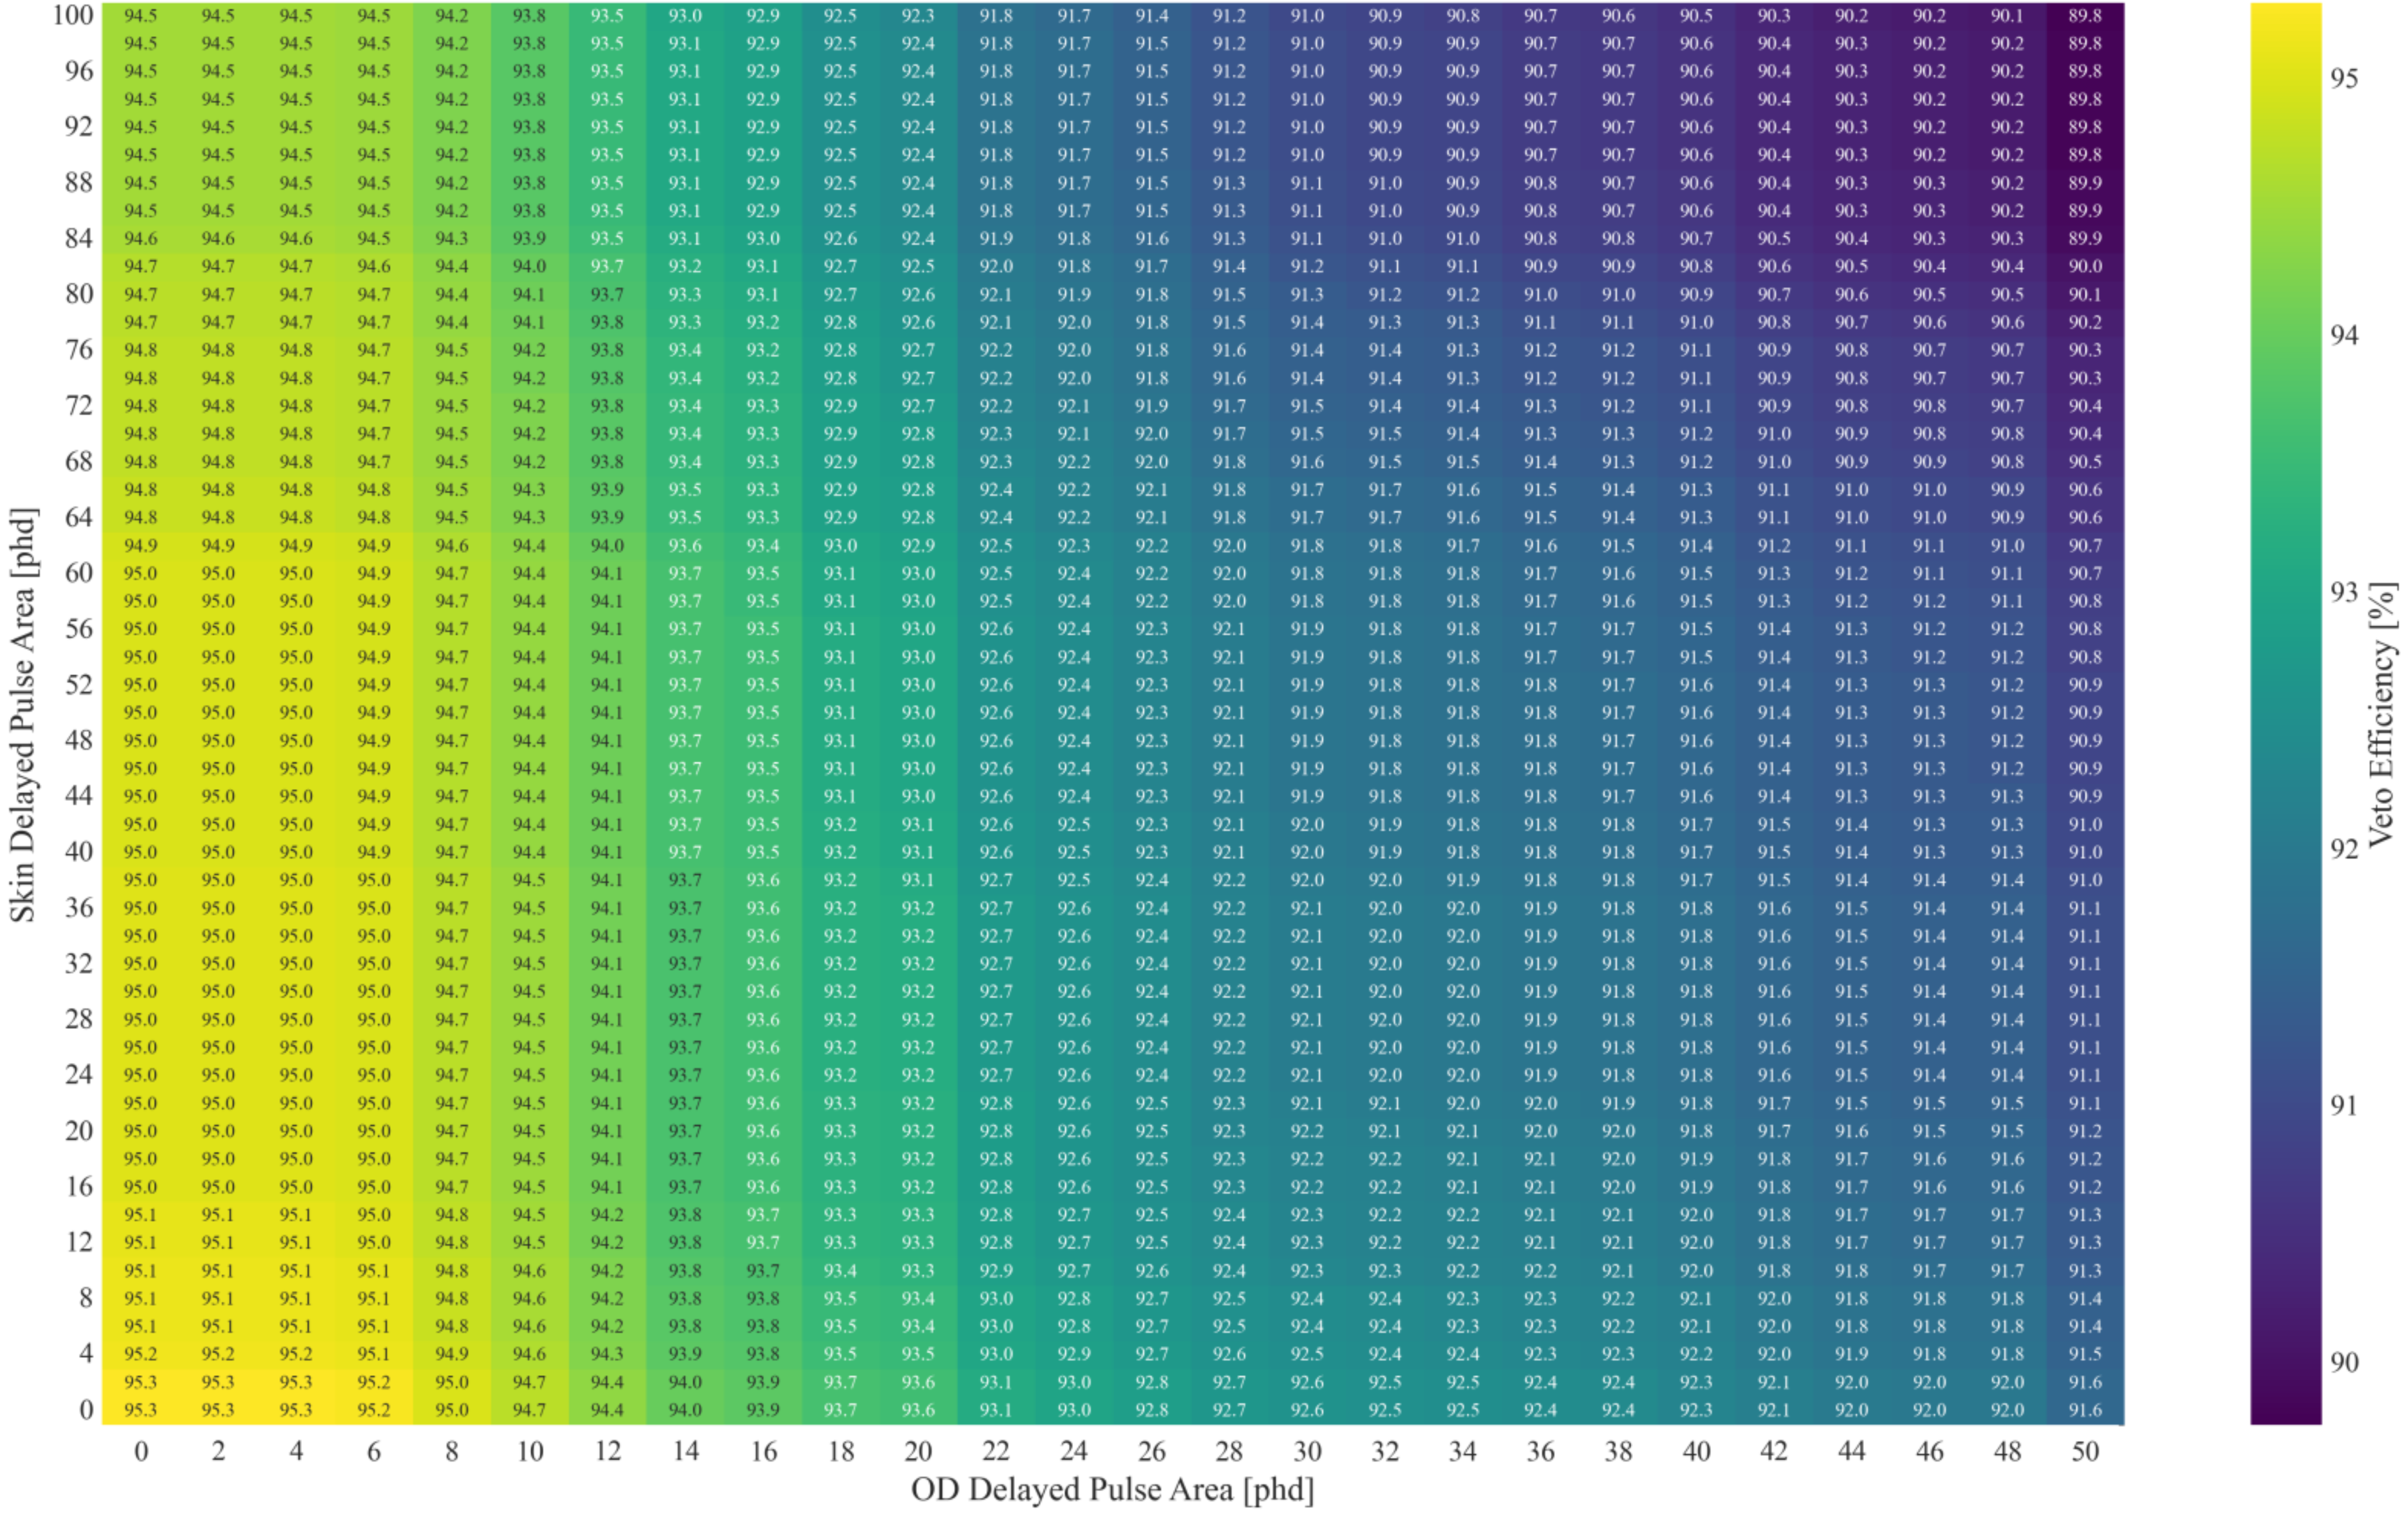
\includegraphics[width=\textwidth]{figures/VetoEfficiency/Heatmap600us_ODDelayedSkinDelayedThresholds.png}
	\caption[Heatmap used to determine optimal OD and Skin Delayed thresholds based on efficiency.]{Heatmap used to determine optimal OD and Skin Delayed thresholds based on efficiency. The $z$-axis shows the efficiency associated with a given pulse area requirement for the delayed veto windows defined in \autoref{tab:VetoEff/sr3_veto_cuts}.}
	\label{fig:VetoEff/od_prompt_veto_heatmap}
\end{figure}

Compiling the heatmaps of efficiency and deadtime for established veto windows of the different criteria, thresholds are chosen to maximise efficiency whilst minimising dead time. An example plot used to determine this is shown in \autoref{fig:VetoEff/veto_cut_optimisation}.
For the WS2024 science run, the approach of trying to maintain the efficiency of WS2022 veto of $\sim$~89\%, whilst reducing the livetime impact is taken. It is determined that the efficiency can be matched to the veto efficiency achieved in the WS2022 science run, whilst achieving a factor of two reduction in deadtime due to the tighter cuts obtained through a better understanding of the veto.

\noindent
The final cuts for the WS2024 science run are shown in \autoref{tab:VetoEff/sr3_veto_cuts}, with the WS2022 selection included for comparison. Any modifications to the selections are shaded to aid the reader's eye.


\begin{figure}[!ht]
	\centering
	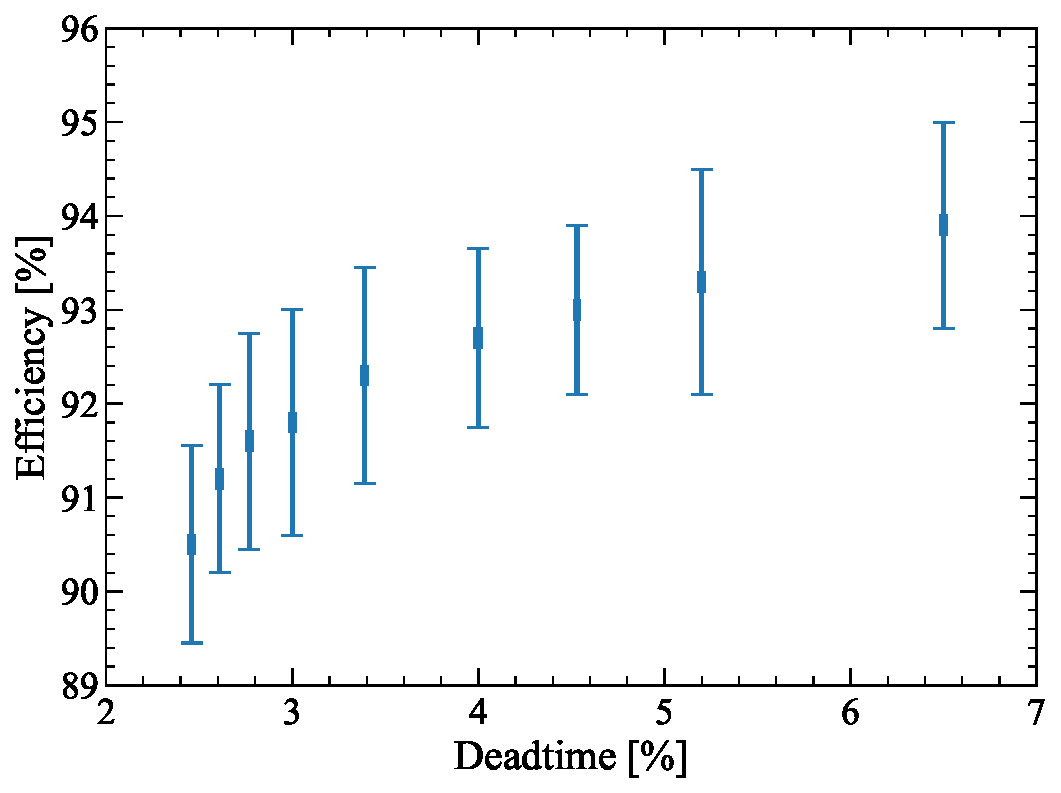
\includegraphics[width=0.7\textwidth]{figures/VetoEfficiency/DeadEffThresholdTest.pdf}
	\caption[Example plot used to highlight a number of considered cuts for the delayed Skin and OD pulse area thresholds for a 600~$\mu$s window.]{Example plot used to highlight a number of considered cuts for the delayed Skin and OD pulse area thresholds for a 600~$\mu$s window. The efficiency values have not been corrected for accidental coincidences (discussed in \autoref{sec:VetoEff/AmLiAccCorrection}). At each point, the numbers in brackets are the OD threshold pulse area and the Skin threshold pulse area.}
	\label{fig:VetoEff/veto_cut_optimisation}
\end{figure}


\begin{table}[!ht]
    \centering
    \caption[Veto coincidence cuts determined to be optimal for the WS2024 science run.]{Veto coincidence cuts determined to be optimal for the WS2024 science run. The WS2022 cuts are also included, where any modifications made to the selections is shaded accordingly.}
    \label{tab:VetoEff/sr3_veto_cuts}
    \scalebox{0.9}{
    \begin{tabular}{|c|c|c||c|c|c|}
    \hline
    \multicolumn{3}{|c||}{\textbf{Skin Prompt}} & \multicolumn{3}{c|}{\textbf{OD Prompt}} \\
    \hline
    & WS2024 & WS2022 & & WS2024 & WS2022 \\
    \hline
    Window & \cellcolor[HTML]{cecece} [-250,250]~ns & \cellcolor[HTML]{cecece}[-500,500]~ns & Window & [-300,300]~ns & [-300,300]~ns\\
    Coincidence&$>2$&$>2$&Coincidence&$>5$&$>5$\\
    Pulse Area & $>2.5$ & $>2.5$ & Pulse Area & \cellcolor[HTML]{cecece}$>4.5$ &\cellcolor[HTML]{cecece} $>0$ \\    
    \hhline{|===||===|}
    \multicolumn{3}{|c||}{\textbf{Skin Delayed}} & \multicolumn{3}{c|}{\textbf{OD Delayed}} \\
    \hline
    &WS2024&WS2022&&WS2024&WS2022\\
    \hline
    Window&\cellcolor[HTML]{cecece}[250~ns, 600~$\mu$s]&\cellcolor[HTML]{cecece}[500~ns, 1200~$\mu$s]&Window&\cellcolor[HTML]{cecece}[300~ns, 600~$\mu$s]&\cellcolor[HTML]{cecece}[300~ns, 1200~$\mu$s]\\
    Coincidence&\cellcolor[HTML]{cecece}$>2$&\cellcolor[HTML]{cecece}$>55$&Coincidence&$>5$&$>5$\\
    Pulse Area&\cellcolor[HTML]{cecece}$>46$&\cellcolor[HTML]{cecece}$>50$&Pulse Area&\cellcolor[HTML]{cecece}$>32.0$&\cellcolor[HTML]{cecece}$>37.5$\\
    \hline
    \end{tabular}}
\end{table}

\subsection{Deadtime stability}\label{sec:VetoEff/DeadtimeStability}
The stability of the induced deadtime for each of the veto selection windows over the WS2024 science run is assessed for stability by comparing the deadtime at monthly intervals. For each month, the rate of pulses in the Skin and OD (above the threshold as defined by the specific veto cut) using randomly triggered data is recorded. The stability of measured deadtime over the WS2024 science run is shown in \autoref{fig:VetoEff/deadtime_stability}.
The deadtime is then calculated as:
\begin{equation}
	\textrm{Dead Time [\%]} = 100 - (\lambda(x)\cdot t_{\text{vw}})
\end{equation}
where $\lambda(x)$ is the background rate above the veto threshold $x$, and $t_{\text{vw}}$ represents the veto window length measured in ns.
The conclusion that the deadtime is stable over the WS2024 science run is confirmed by measuring the rate of OD pulses above $200~\text{keV}$ (as defined by the WS2022 energy calibration) using the \lstinline{ODHealth} PREM module. No significant fluctuation is observed during the WS2024 science run, shown in \autoref{fig:VetoEff/deadtime_stability_prem}.
\begin{figure}[!h]
	\centering
	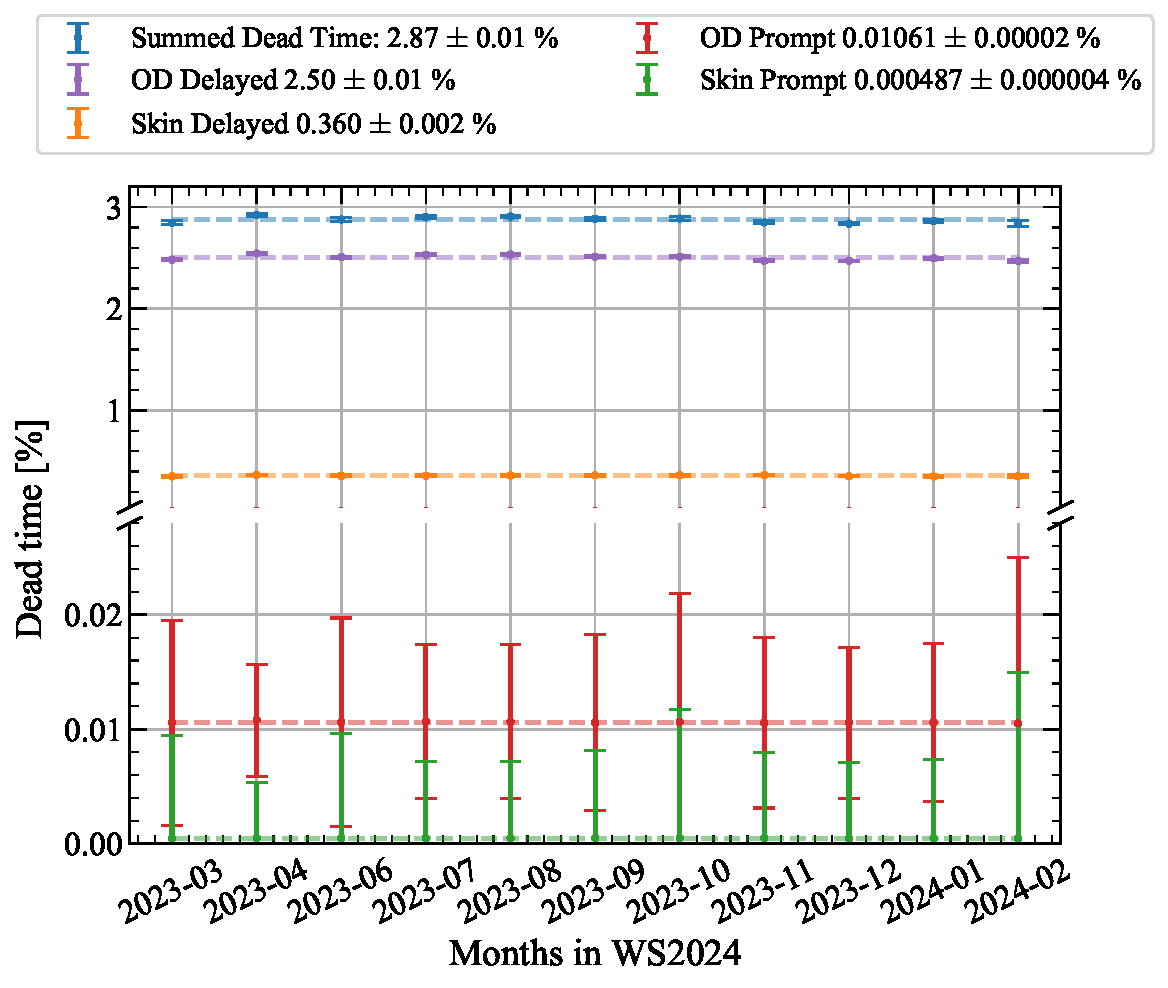
\includegraphics[width=0.7\textwidth]{figures/VetoEfficiency/SR3DeadTimeAll_withMean.pdf}
	\caption[Deadtime from the Skin and OD veto selection criteria during each month of WS2024 science run.]{Deadtime from the Skin and OD veto selection criteria during each month of WS2024 science run. The error shown is purely statistical, and the mean across the science run is shown by a dashed line.}
	\label{fig:VetoEff/deadtime_stability}
\end{figure}
\begin{figure}[!h]
	\centering
	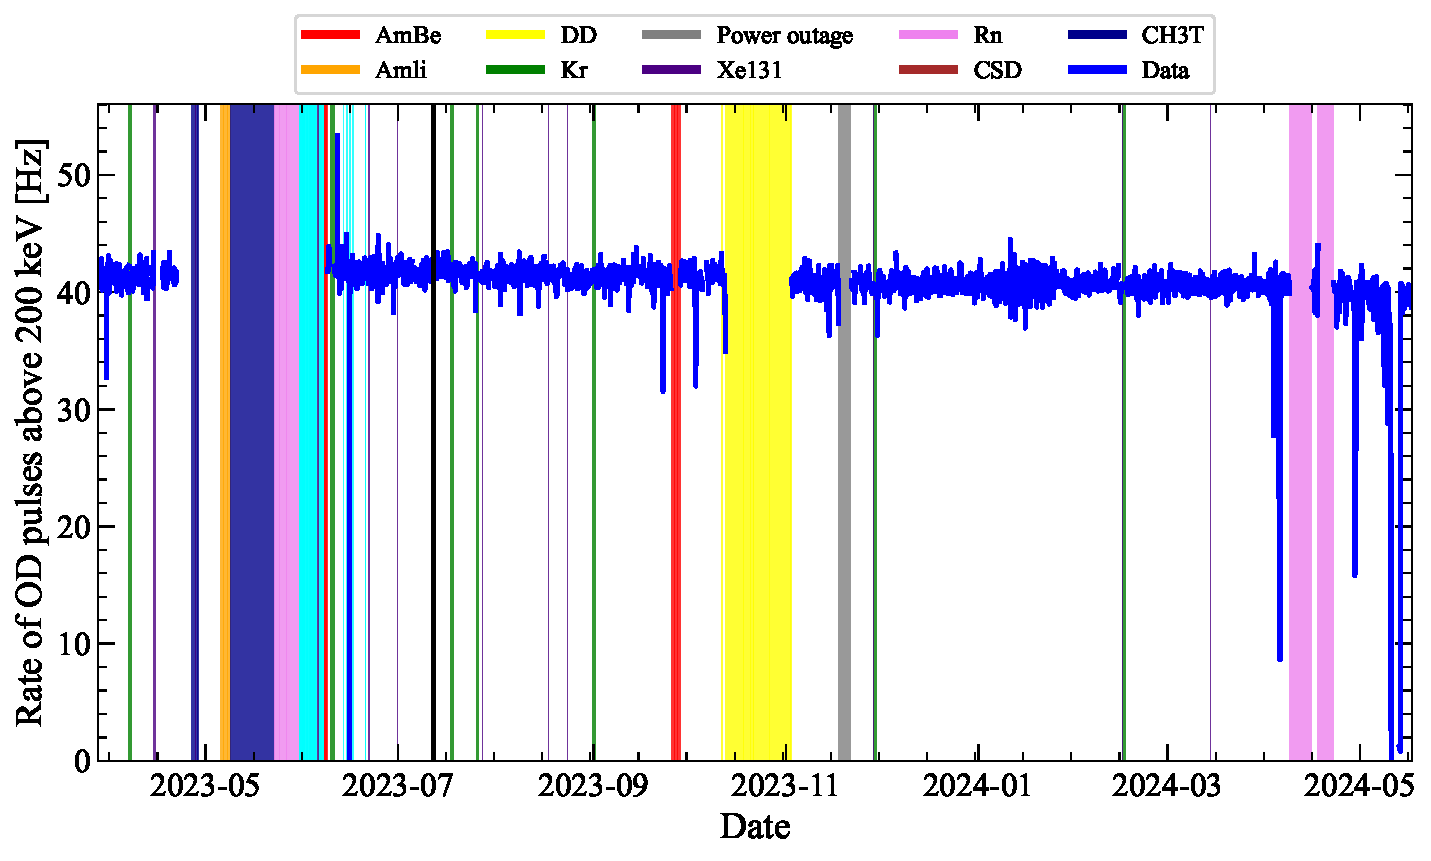
\includegraphics[width=\textwidth]{figures/VetoEfficiency/prem_od_stability.pdf}
	\caption[Rate of OD pulses above 200~keV over the WS2024 science run.]{Rate of OD pulses above 200~keV (as defined by WS2022 energy calibration) over the WS2024 science run. Various periods of calibration are indicated by the coloured regions. The vertical black line indicates a change in the state of xenon circulation in the TPC.}
	\label{fig:VetoEff/deadtime_stability_prem}
\end{figure}

\section{Neutron veto efficiency}\label{sec:VetoEff/efficiency}
To estimate the neutron background of LZ during a science run, we must know what fraction of neutron-induced NR single scatters produce a signal in the veto detectors. We call this quantity the \textit{veto efficiency}.
In this section, the efficiency of tagging background neutrons using the Skin and OD detectors is calculated.
This is performed by calculating the efficiency on AmLi and DD calibration data and comparing to simulations.
The difference between efficiencies from simulations and data is then used to calculate an offset factor.
The efficiency is then calculated for detector NR simulations, and the observed offset factor is used to estimate the tagging efficiency for events classified as detector NR \cite{LZ:2022ysc,LZ:2024zvo}.
The efficiency is defined as:
\begin{equation}\label{eqn:VetoEff/neutron_tagging_efficiency}
	\eta\;[\%] = \frac{\textrm{Events passing TPC analysis cuts + veto cuts}}{\textrm{Events passing TPC analysis cuts}} \times 100
\end{equation}
and the inefficiency is defined as $\cancel{\eta}=100-\eta$. For all veto efficiency calculations in this chapter, if a pulse in the Skin or OD passes any of the selections outlined in \autoref{tab:VetoEff/sr3_veto_cuts}, then the event is included in the number of events in the numerator of \autoref{eqn:VetoEff/neutron_tagging_efficiency}. The efficiency based on this decision logic is the \textit{total veto efficiency}.

Two additional efficiencies are investigated: \textit{delayed veto efficiency} defined as events where a pulse is observed that fulfils either of the Skin delayed or OD delayed selection criteria, denoted by $\eta_\text{delayed}$; and \textit{OD-delayed veto efficiency} defined as events where a pulse is observed that fulfils the OD delayed selection criteria, denoted by $\eta_\text{OD-delayed}$.

Unless otherwise stated, all veto efficiencies presented follow the \textit{total veto efficiency} logic.

\subsection{Neutrons from calibration sources}\label{sec:VetoEff/NeutronsFromCalibrationSources}
LZ utilises two neutron sources, AmLi and a deuterium-deuterium (DD) neutron generator, to calibrate the detector response to nuclear recoils and to measure the neutron tagging efficiencies of the veto detectors. The following two sections will detail the veto calculation for each of the calibration data sets.

\subsubsection{AmLi}\label{sec:VetoEff/AmLi_Efficiency}
AmLi sources are a compound of \textsuperscript{241}Am $\alpha$-radioactivity and \textsuperscript{7}Li produces low-energy neutron emission via nuclear $(\alpha,\text{n})$ reactions. Alphas from $^{241}$Am decay bombard the $^{7}$Li nuclei. This leads to a nuclear reaction of type \textsuperscript{7}Li$+\alpha \rightarrow$\textsuperscript{11}B\textsuperscript{*}. The excited \textsuperscript{11}B nucleus then decays to \textsuperscript{11}B via neutron emission. The neutrons produced by the AmLi sources have a maximum energy of $\sim1.5~\text{MeV}$, which results in a nuclear recoil depositing up to $\sim45~\text{keV}_{nr}$ of energy \cite{LZ:2024bsz}. Gamma radiation is also emitted in the \textsuperscript{241}Am decay to various states of \textsuperscript{237}Np and is an associated background to the reaction neutrons. The neutron to gamma ray emission ratio is 0.032 \cite{Sazzad:2023uqs}. The gamma ray background of the AmLi source is accounted for by the accidental correction factors described later in this section. The characterisation of the LZ AmLi sources is discussed in detail in Ref.~\cite{Sazzad:2023uqs}.

The AmLi calibration data used in this study were taken during the May 2023 calibration campaign before the WS2024 science run. Events which are classified as single scatters by LZap and pass the selection outlined in \autoref{tab:VetoEff/amli_efficiency_cuts} are used for the study. Two additional cuts are applied to the calibration data:
\begin{enumerate}
	\item \textit{CSD tube position selection:} A circular cut on the reconstructed position of the SS S1 pulse in the TPC, such that events from just one CSD tube are selected at a time. During the calibration campaign, sources were simultaneously deployed in each of the CSD tubes at equal heights (three separate height positions were used, $z=100~\text{mm},700~\text{mm},1300~\text{mm}$ relative to the cathode at $z=0~\text{mm}$). Whereas separate simulations were produced with a single source in each CSD tube at three different heights (equal to the $z$-position used in the calibration campaign).
    The circular cut selects events that have an SS S1 reconstructed position within a 50~mm radius of the CSD tube using the following equation:
    \begin{equation}\label{eqn:VetoEff/CSDSelection}
        \sqrt{(\text{S1}_x-\text{CSD}_x^i)^2+(\text{S1}_y-\text{CSD}_y^i)^2}<50,
    \end{equation}
    where S1$_{x,y}$ is the reconstructed $(x,y)$-position of the S1 pulse in the SS and $\text{CSD}_{x,y}^i$ is the $(x,y)$-position of CSD where $i=1,2,3$ for each of the three CSD tubes.
    The boundaries of the cuts for each of the CSD tubes is shown in \autoref{fig:VetoEff/CSDSelection}. 
    \begin{figure}[!ht]
    \centering
        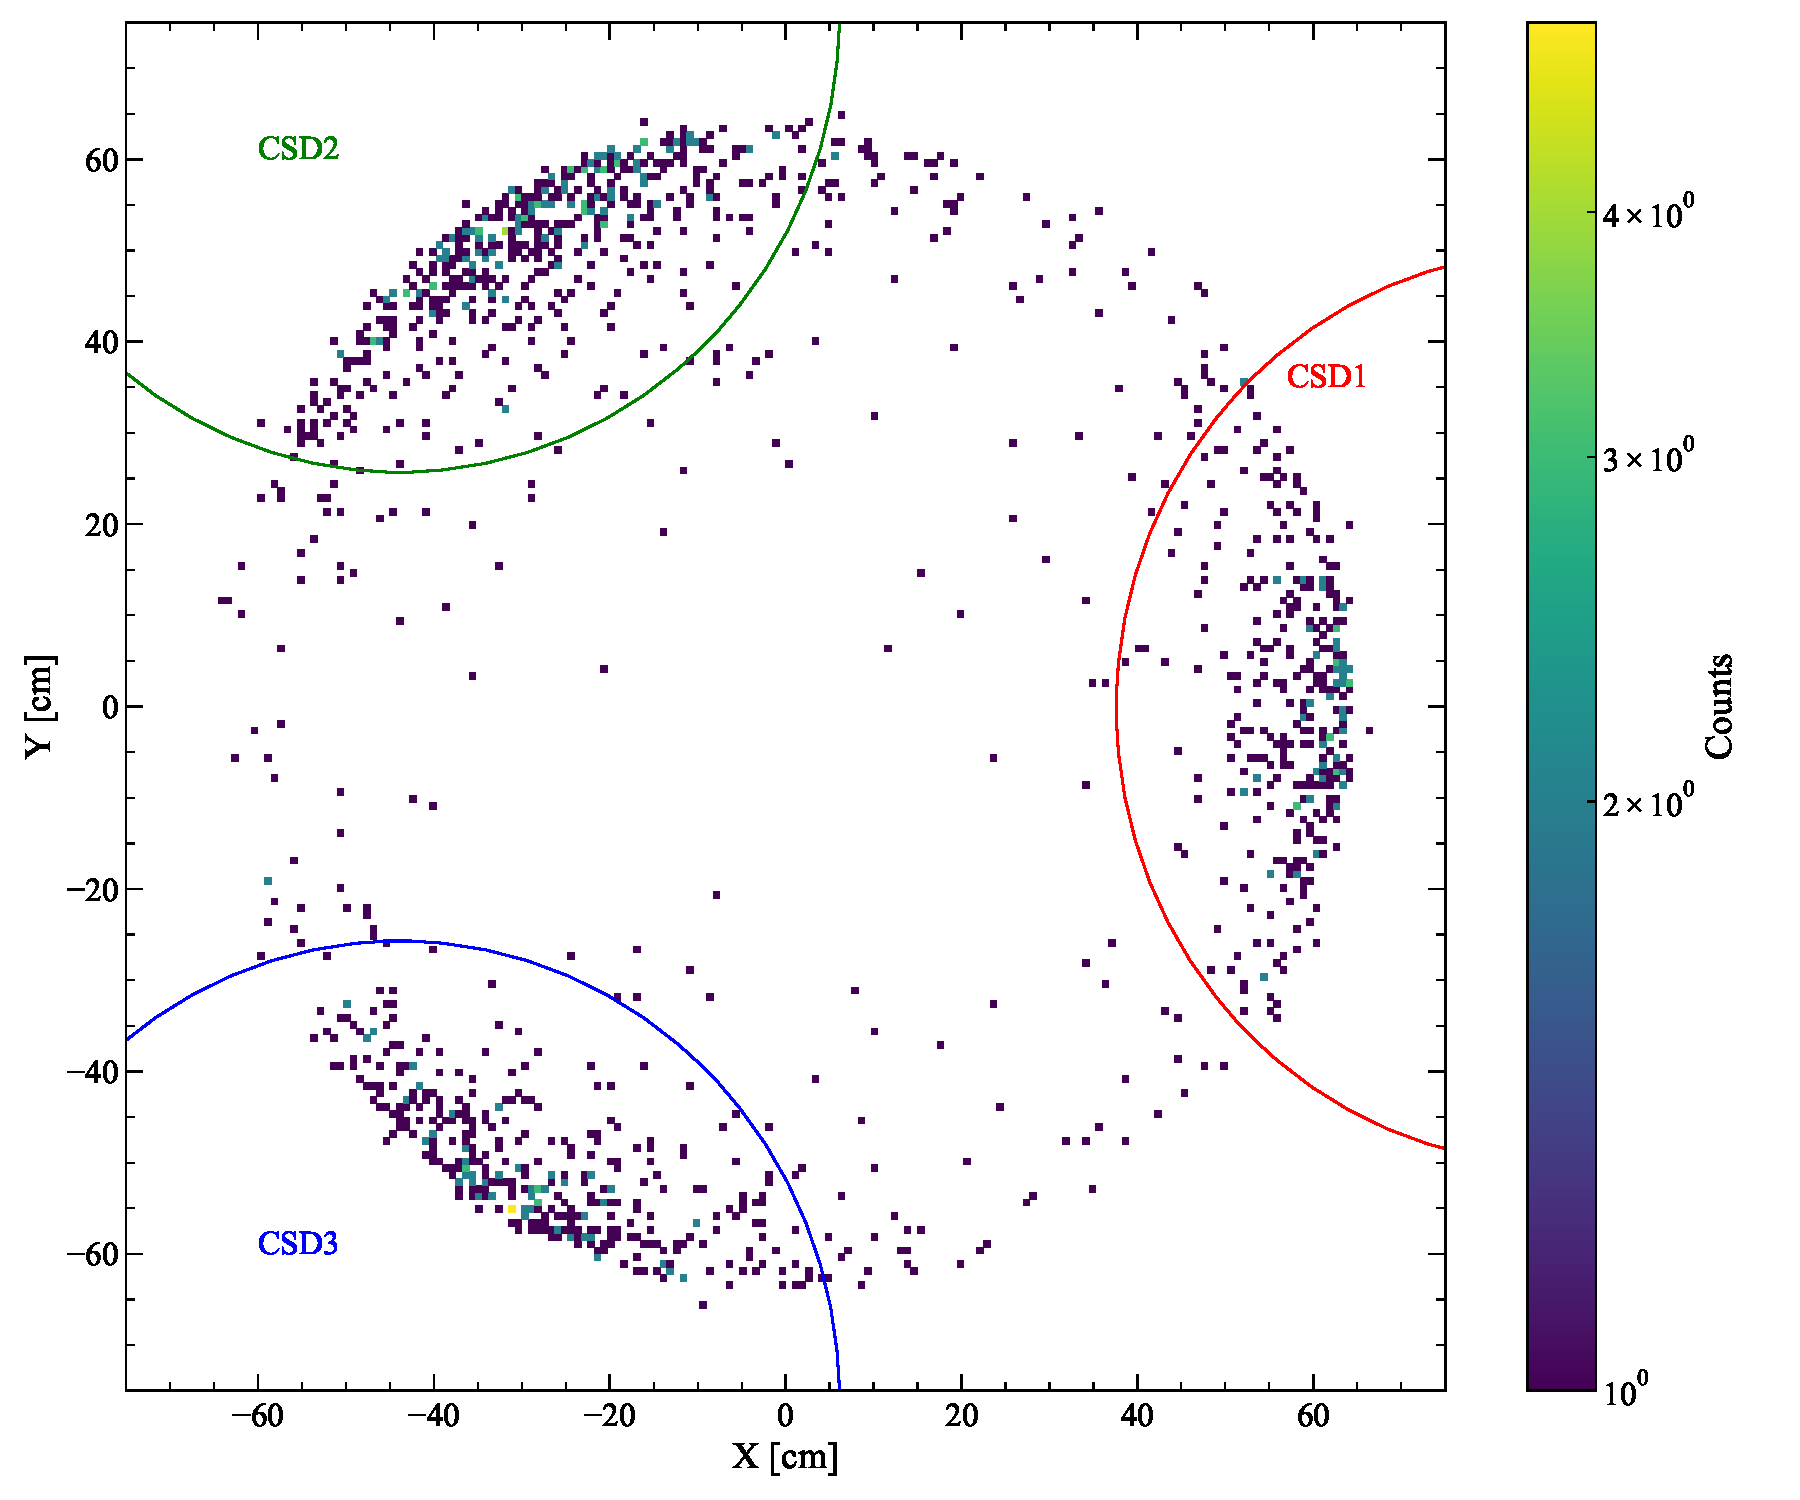
\includegraphics[width=0.7\textwidth]{figures/VetoEfficiency/CircularCSDCut.pdf}
        \caption[X-Y distribution of SS S1 pulses in the TPC for AmLi sources positioned at 700mm.]{X-Y distribution of SS S1 pulses in the TPC for AmLi sources positioned at 700mm. Each of the circular cuts are overlaid on the plot.}
        \label{fig:VetoEff/CSDSelection}
    \end{figure}
    
    The position dependence of the veto efficiency can be examined by applying the CSD tube selection to data collected at different $z$-positions. The veto efficiency for different CSD tubes and $z$-positions is shown in \autoref{fig:VetoEff/VetoEffPositionDependence}.
    
    \begin{figure}[!h]
    	\centering
    	\begin{subfigure}[b]{0.49\textwidth}
    		\centering
    		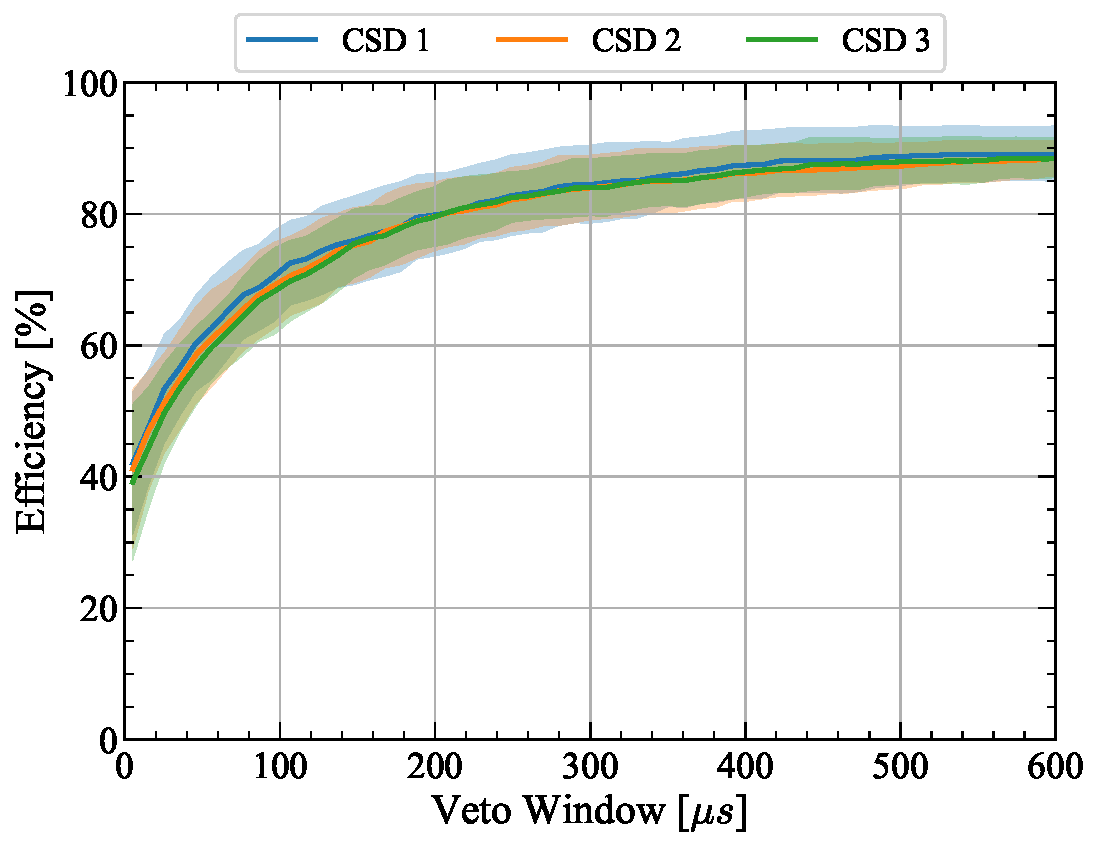
\includegraphics[width=\textwidth]{figures/VetoEfficiency/Eff_AmLi_Total_AllCSD.pdf}
    		\caption{}
            \label{fig:VetoEff/VetoEffPositionDependenceZPos}
    	\end{subfigure}
    	\hfill
    	\begin{subfigure}[b]{0.49\textwidth}
    		\centering
    		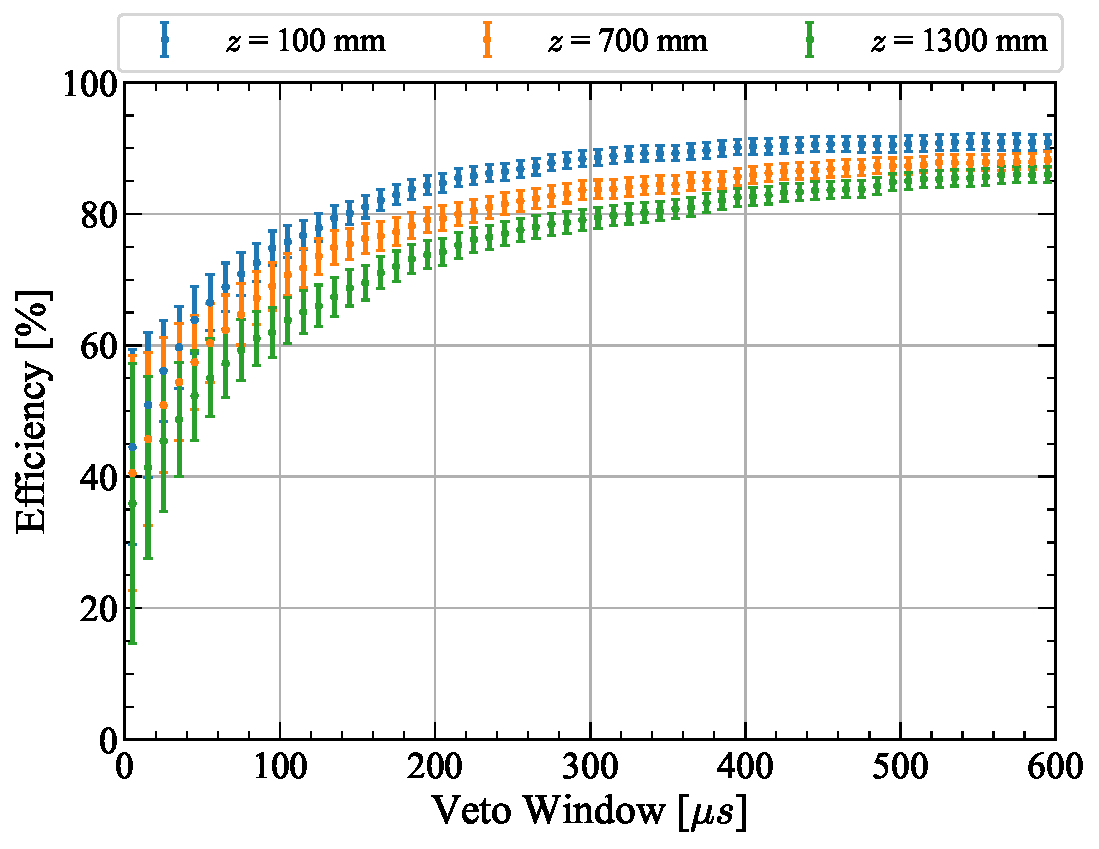
\includegraphics[width=\textwidth]{figures/VetoEfficiency/Eff_AmLi_Total_AllHeights.pdf}
            \caption{}
    		\label{fig:VetoEff/VetoEffPositionDependenceCSD}
    	\end{subfigure}
    	\caption[Position dependent veto efficiencies for different CSD tubes (left) and $z$-positions (right).]{Position dependent veto efficiencies for different CSD tubes (left) and $z$-positions (right). The bands for each trace correspond to 1$\sigma$ statistical errors on the efficiency measured.}
    	\label{fig:VetoEff/VetoEffPositionDependence}
    \end{figure}
    
	A concern of this cut is that events towards the centre of the TPC are excluded from the veto efficiency measurement, biasing the measured efficiency to events closer to the wall of the TPC. When the efficiency is averaged across different heights and CSD tube, the average can then be replicated in both data and simulation. 
    The position-averaged efficiency when the CSD cut is applied and without a cut is compatible, at  $(88.21\pm1.03)\%$ and $(88.25\pm1.22)\%$ respectively.
	The cut has $<5\%$ impact across the veto window and $<0.1\%$ impact at the 600~$\mu$s veto window threshold. This comparison is shown in \autoref{fig:VetoEff/CSDSelectionEffComp}.
    \begin{figure}[!h]
    	\centering
    	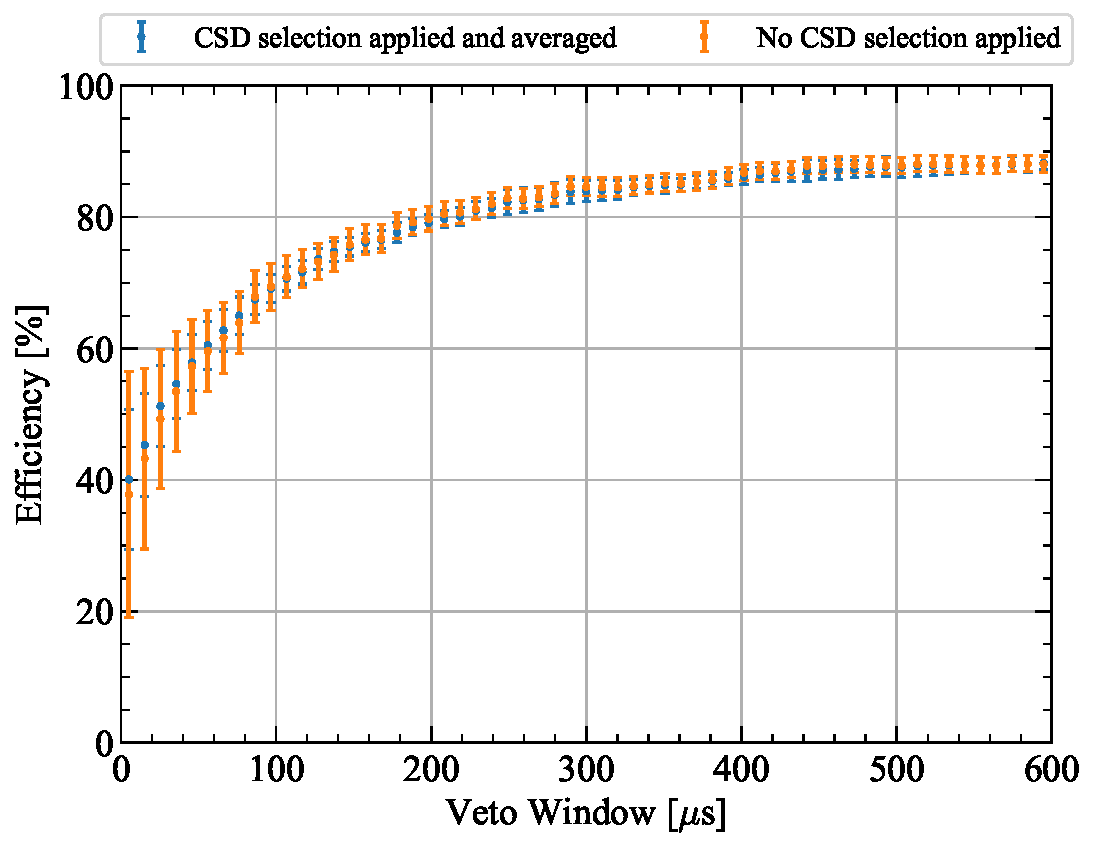
\includegraphics[width=0.7\linewidth]{figures/VetoEfficiency/CSDSelectionCheck.pdf}
    	\caption[CSD tube selection impact on veto efficiency.]{CSD tube selection impact on veto efficiency. The average veto efficiency for events that have a reconstructed position with 50~mm of a CSD tube (blue) is compared to the veto efficiency of all events with no CSD selection applied. The cut has $<5\%$ impact across the veto window and $<0.1\%$ impact at the 600~$\mu$s veto window threshold.}
    	\label{fig:VetoEff/CSDSelectionEffComp}
    \end{figure}

	\item \textit{NR-band selection:} SS events which have an S1 and S2 pulse area that lie within 1-$\sigma$ of NR band mean are selected for the veto efficiency calculation.
    The NR bands generated using the Noble Element Simulation Technique (NEST) \cite{NEST2011} are shown in \autoref{fig:VetoEff/SR3NRBands}. As discussed in \autoref{sec:LZ/NRERDiscrim}, the ratio between S1 and S2 light is used for ER and NR discrimination. This discrimination can be seen clearly by the spacing between the ``Flat beta ER'' band and the NR bands from AmLi and DD. The NR bands of AmLi and DD differ from each other due to the energy of the neutrons emitted by the sources and the corresponding energy deposited in the single scatter interactions.
    The selection is defined as:
    \begin{equation}\label{eqn:VetoEff/NRBandSelection}
        -1<\frac{\textrm{log}_{10}(\text{S2}_\text{obs.})-\overline{\textrm{log}_{10}(\text{S2})}(\text{S1}_\text{obs.})}{\sigma_{\textrm{log}_{10}(\overline{\text{S2}})}(\text{S1}_\text{obs.})}<1,
    \end{equation}
    where $\text{S1}_\text{obs.}$ and $log_{10}(\text{S2}_\text{obs.})$ are the observed pulse areas from the SS, $\overline{log_{10}(\text{S2})}(\text{S1}_\text{obs.})$ is the mean S2 corresponding to a observed S1 with $\sigma_{log_{10}(\overline{\text{S2}})}(\text{S1}_\text{obs.})$ based on the NEST model. The purpose of this cut is to improve the purity of the selection and retain 63\% of the data.
    \begin{figure}[!ht]
    \centering
    \begin{subfigure}[b]{0.49\textwidth}
        \centering
        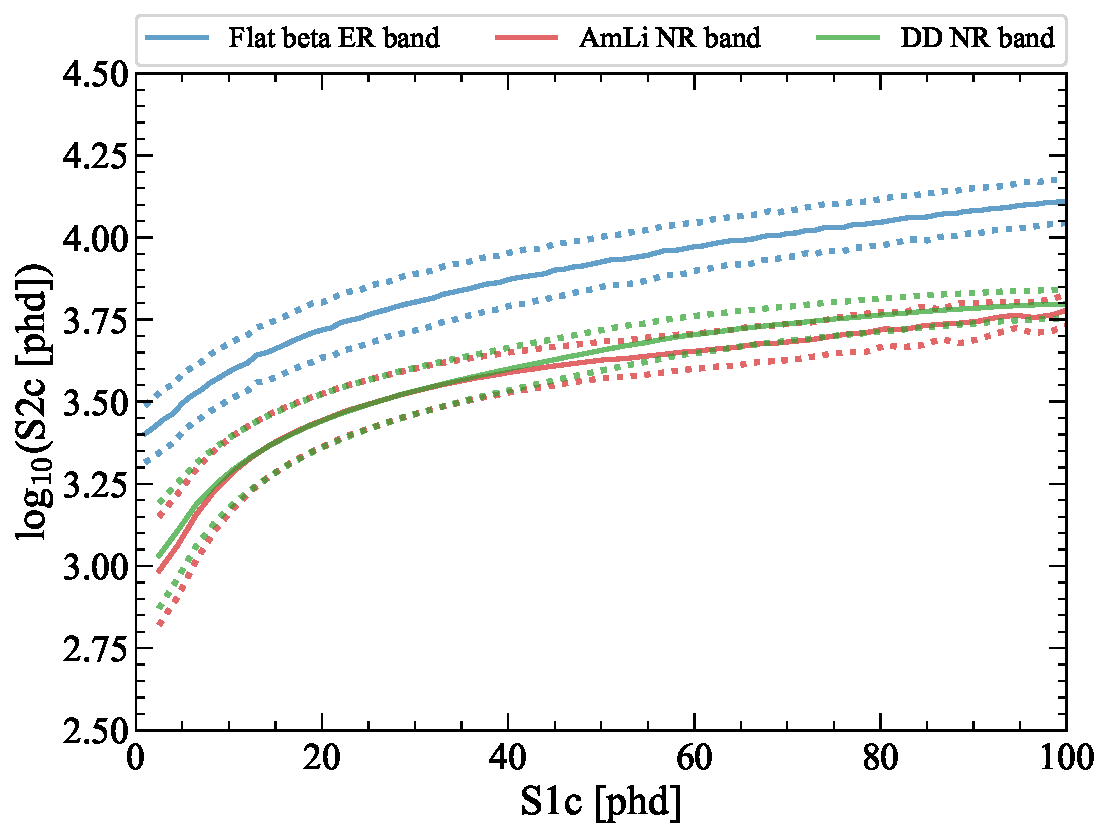
\includegraphics[width=\textwidth]{figures/VetoEfficiency/NRBands.pdf}
        \caption{}
        \label{fig:VetoEff/SR3NRBands}
    \end{subfigure}
    \hfill
    \begin{subfigure}[b]{0.49\textwidth}
        \centering
        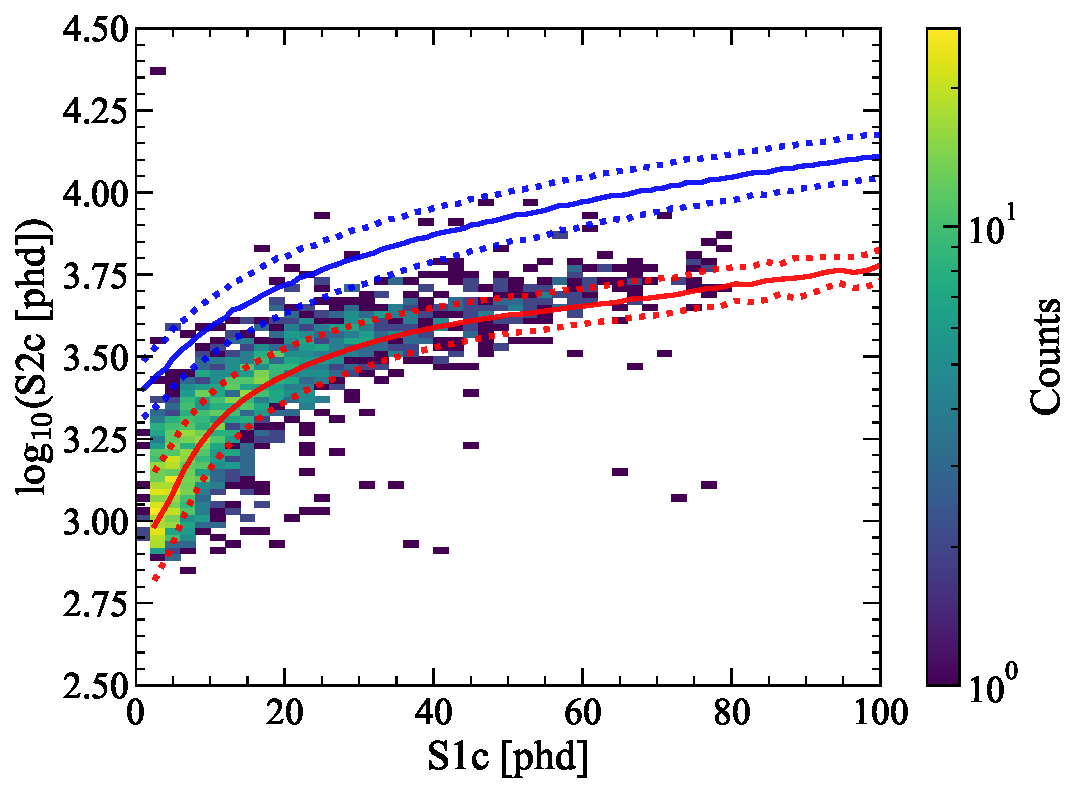
\includegraphics[width=\textwidth]{figures/VetoEfficiency/AmLi700_NRBands.pdf}
        \caption{}
        \label{fig:VetoEff/AmLi700_NRBands}
    \end{subfigure}
    \caption[NR and ER bands for the flat beta ER, AmLi NR, and DD NR models alongside a plot of AmLi calibration data with the corresponding NR bands overlaid.]{\textbf{Left:} The NR band means (solid line) with 1-$\sigma$ boundaries (dashed lines) for AmLi and DD calibration sources and a flat beta ER band mean with 1-$\sigma$ boundary. Both NR and ER bands and 1-$\sigma$ boundaries were generated using NEST. \textbf{Right:} AmLi calibration data at $z=700~\text{mm}$ with the corresponding NR band mean and 1-$\sigma$ boundary overlaid.}
    \label{fig:VetoEff/SR3NRBands&AmLi700mmData}
\end{figure}
\end{enumerate}

\subsubsection{Accidental correction factor calculation}\label{sec:VetoEff/AmLiAccCorrection}
If, during the calibration, neutrons and gamma rays cause additional veto signals when an unconnected NR event is recorded in the TPC, the veto efficiency will be overestimated. In this chapter, I will call these events \textit{accidental coincidences}\footnote{In LZ, accidental coincidences are also used as a term for spuriously paired S1 and S2 false events, but this is not a concern in this chapter.}. To account for this, we estimate the rate of such non-connected vetoes with a sample of events from the calibration dataset randomly triggered in time. Neutrons, which are associated with accidental coincidences, are produced via additional $(\alpha,\text{n})$ reactions of the AmLi source, whilst gamma rays are produced from neutron capture on Gd and H in the GdLS. A small percentage of gamma rays are produced by the $\alpha$ decay of \textsuperscript{241}Am \cite{Sazzad:2023uqs}.

We define the probability of no veto signal in the absence of a TPC interaction as $P(a=0)$, where $a$ is the number of veto detectors observing a pulse. We also define the true veto inefficiency $\cancel\eta_\text{true}$ as the probability, given a TPC interaction, that no veto signal is caused by the neutron that caused \emph{the interaction in the TPC}. Since in $1-P(a=0)$ of cases, such an event will have a spurious veto, the observed veto inefficiency will be $\cancel\eta_\text{obs.}=P(a=0)\cdot\cancel\eta_\text{true}$. The observables are the number of TPC SS NR events $N$, the number of those events without a veto signal $M$, the number of randomly triggered `events' $N_\text{random}$, and the number of times a randomly triggered event without a veto signal $M_\text{random}$, giving:

\begin{align}
    \cancel\eta_\text{obs.}&=\frac{M}{N}\\
    P(a=0)&=\frac{M_\text{random}}{N_\text{random}}\\
    \hat{\cancel\eta}&=\frac{\cancel\eta_\text{obs.}}{P(a=0)}\\
    &=\frac{M/N}{M_\text{random}/N_\text{random}},
\end{align}

where $\hat{\cancel\eta}$ is the estimated veto inefficiency for a given veto selection. The accidental correction and veto efficiency are correlated with the length of the veto window and veto pulse thresholds. Scans over the entire delayed veto window in 10~$\mu$s steps to observe the change in the correction factor over time are shown in \autoref{fig:VetoEff/SR3AmLi_700mm_Corrections}. The probability of observing zero accidental pulses in the veto detector decreases with increasing veto window size. The probability of observing a coincident neutron from the AmLi or a gamma from neutron capture on Gd and H in the GdLS increases with veto window size. At the chosen delayed cut window length of 600~\textmu s, $P(a=0)=0.79\pm0.03$. 
The impact of the accidental correction when applied to the observed efficiency is shown in \autoref{fig:VetoEff/AmLiAccidentalCorrectionImpact}. The impact can be as large as 20\% at large cut windows.

\begin{figure}[!ht]
    \centering
    \begin{subfigure}[b]{0.49\textwidth}
        \centering
        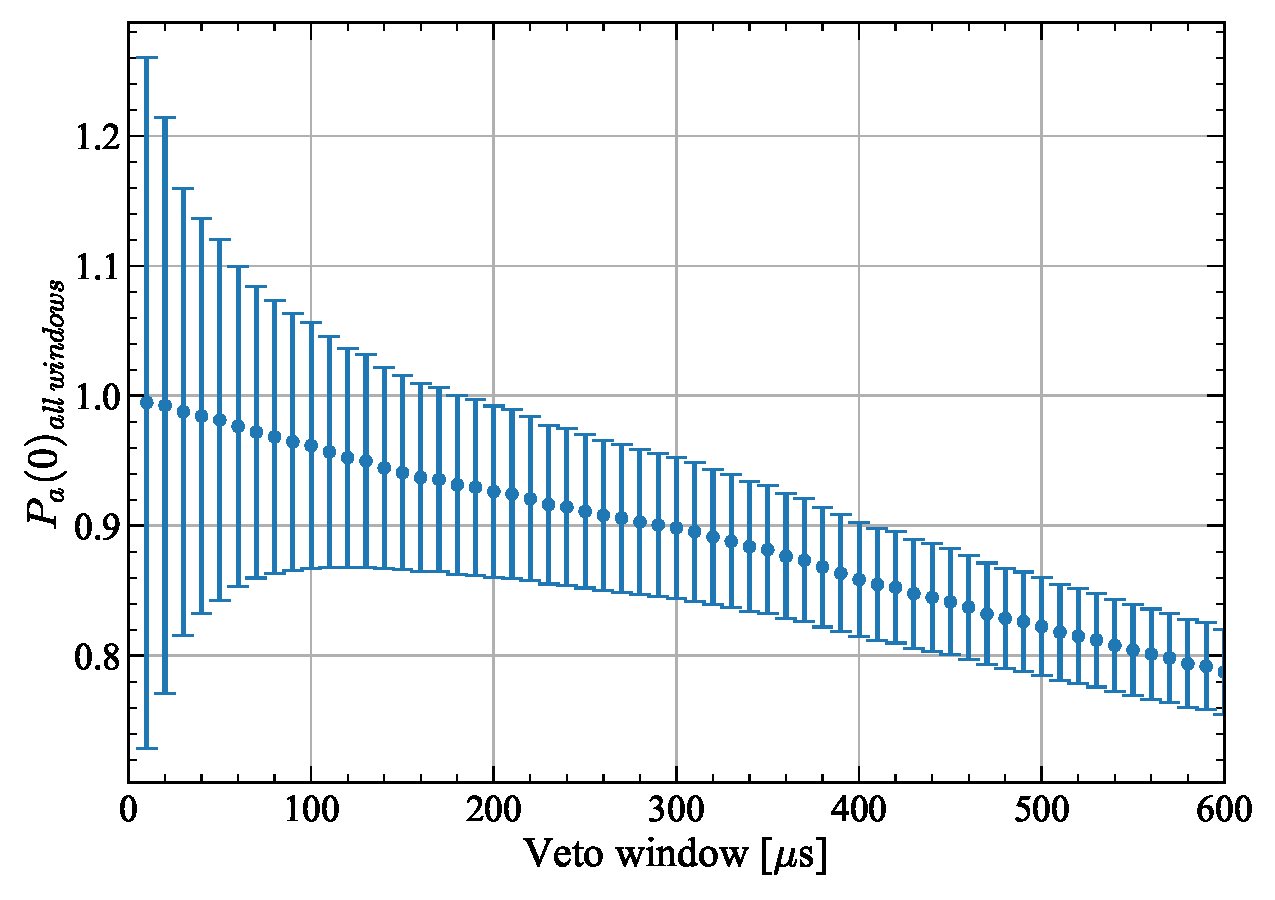
\includegraphics[width=\textwidth]{figures/VetoEfficiency/SR3AmLi_700mm_Corrections_100k.pdf}
        \caption{}
        \label{fig:VetoEff/SR3AmLi_700mm_Corrections}
    \end{subfigure}
    \hfill
    \begin{subfigure}[b]{0.49\textwidth}
        \centering
        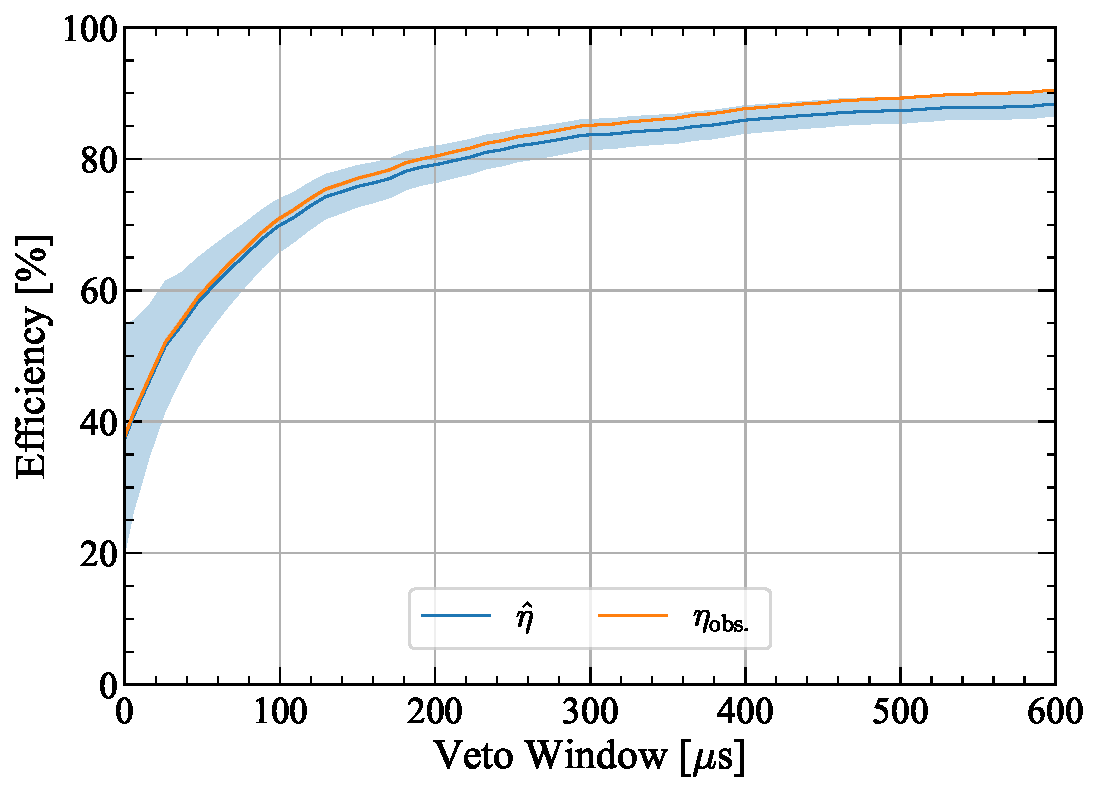
\includegraphics[width=\textwidth]{figures/VetoEfficiency/AmLiAccidentalCheck.pdf}
        \caption{}
        \label{fig:VetoEff/AmLiAccidentalCorrectionImpact}
    \end{subfigure}
    \caption[$P(a=0)$ accidental correction factors over a 600~\textmu s for AmLi calibration sources positioned at $z=700~\text{mm}$ alongside the veto efficiency with the corrections applied.]{\textbf{Left:} $P(a=0)$ accidental correction factors over a 600~\textmu s for AmLi calibration sources positioned at $z=700~\text{mm}$. The errors shown are only statistical uncertainties. \textbf{Right:} Comparison between calculated veto efficiencies for AmLi calibration sources positioned at $z=700~\text{mm}$ with accidental correction applied, $\hat{\eta}$, and not applied, $\eta_\text{obs.}$.}
    \label{fig:VetoEff/AmLiAccidentalPlots}
\end{figure}
The final efficiencies measured using AmLi calibration data, corrected for accidental coincidences, and averaged across all positions are shown in \autoref{fig:VetoEff/AmLiEfficiencies}. At the nominal 600~\textmu s veto window, $\eta^\text{Total}_\text{Data}=(89\pm3)\%$, $\eta^\text{Delayed}_\text{Data}=(83\pm3)\%$, and $\eta^\text{OD Delayed}_\text{Data}=(76\pm2)\%$.

\begin{figure}[!ht]
    \centering
    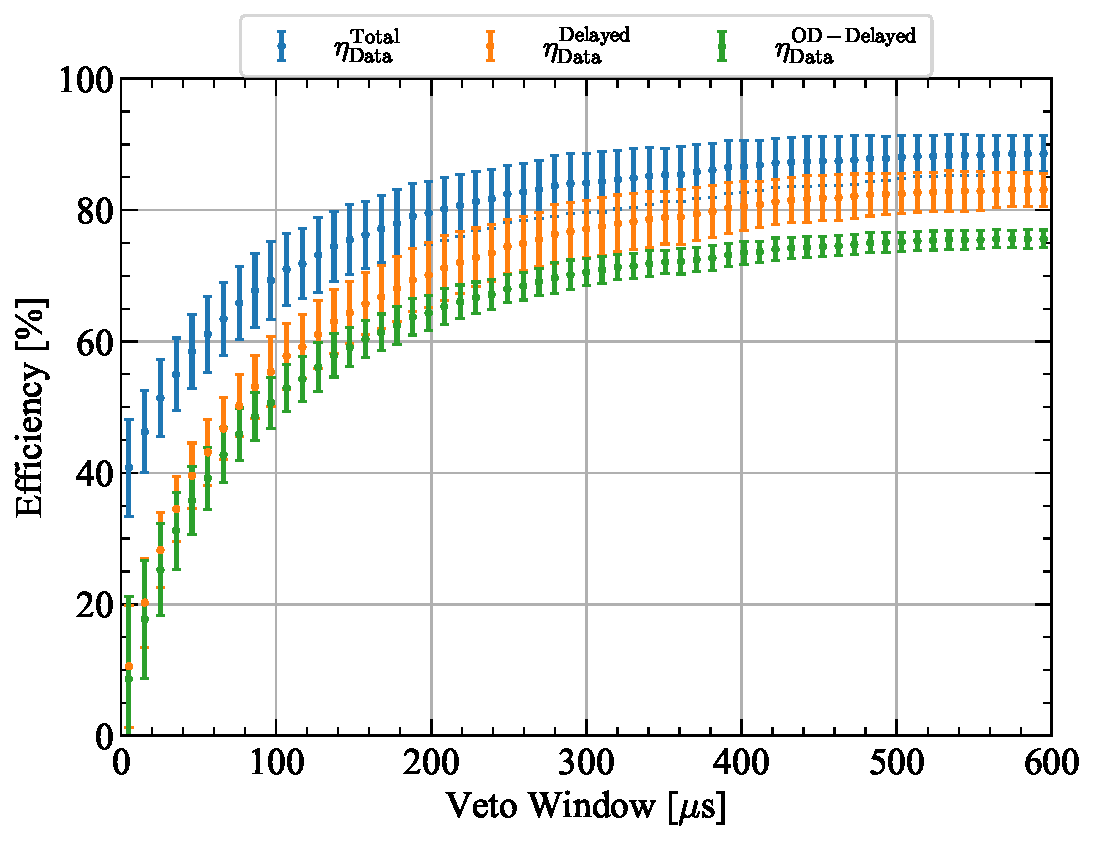
\includegraphics[width=0.7\textwidth]{figures/VetoEfficiency/AmLiEfficiencies_Data.pdf}
    \caption[Final efficiencies measured using AmLi calibration data, corrected for accidental coincidences.]{Final efficiencies measured using AmLi calibration data, corrected for accidental coincidences, and averaged across all positions. At the nominal 600~\textmu s veto window, $\eta^\text{Total}_\text{Data}=(89\pm3)\%$, $\eta^\text{Delayed}_\text{Data}=(83\pm3)\%$, and $\eta^\text{OD Delayed}_\text{Data}=(76\pm2)\%$.}
    \label{fig:VetoEff/AmLiEfficiencies}
\end{figure}

\subsubsection{Deuterium-deuterium neutron generator}
A deuterium-deuterium (DD) neutron generator is used to produce mono-energetic 2.46~MeV neutrons, which result in nuclear recoils depositing up to $74~\text{keV}_{nr}$ of energy. Neutrons are produced by the DD generator as follows: Deuterium is ionized and turned into a plasma by a microwave. Deuterium ions in the plasma are accelerated towards a charged titanium-coated copper target. D\textsuperscript{+} ions embed into the target form of titanium deuteride. Subsequent D\textsuperscript{+} ions fuse to the embedded ions and release neutrons via the D+D$\rightarrow$\textsuperscript{3}He+n. The generator is positioned outside of the water tank, and neutrons are collimated and transmitted to the OCV through nitrogen-purged conduits \cite{LZ:2024bsz}. The neutron production is pulsed to suppress the ER background rate and enables the selection of events coincident with neutron production. Neutron pulsing decreases the impact of accidental coincidences, which artificially increases the veto tagging efficiency. Accidental correction factors are still required as pulsing neutron production does not completely suppress accidental coincidences.

The DD calibration data used in this study were taken during the October 2023 calibration campaign before the WS2024 science run. Events which are classified as single scatters by LZap and pass the selection outlined in \autoref{tab:VetoEff/dd_efficiency_cuts} are used for the study. In addition to these cuts, an NR band selection, defined by \autoref{eqn:VetoEff/NRBandSelection}, is applied. It is important to note that the DD NR band is different from the AmLi NR band. The two different NR bands for the calibration sources are shown in \autoref{fig:VetoEff/SR3NRBands}.

\begin{table}[!ht]
	\centering
	\caption[Outline of cuts applied to DD calibration data for determining the veto efficiency.]{Outline of cuts applied to DD calibration data for determining the veto efficiency. All cuts are defined in \autoref{sec:app/WSCoreCuts}.}
	\begin{tabular}{lll}
    \hline\hline
	\textbf{Physics cuts}&\textbf{S2 cuts}&\textbf{S1 cuts} \\
	\hline
	Single scatter & S2 width vs drift time & S1 Stinger \\
	S1 threshold & Narrow S2 & S1 TBA vs drift time  \\
	S2 threshold & S2 rise time & S1 HSC cut \\
    Fiducial volume & S2 early peak & S1 Shape \\
	NR Band Selection (defined in \autoref{eqn:VetoEff/NRBandSelection})& S2 XY quality & \\
	& S2 TBA & \\
    \hline\hline
	\end{tabular}
	\label{tab:VetoEff/dd_efficiency_cuts}
\end{table}
The DD calibration data is also corrected for accidental coincidences. The same method is used, which is discussed in \autoref{sec:VetoEff/AmLiAccCorrection}. The correction factors used as a function of veto window are shown in \autoref{fig:VetoEff/DDAccCorrectionParameters}. At the nominal 600~\textmu s veto window, $P(a=0)=0.88\pm0.11$. The impact of accidental coincidences on DD data is significantly less than AmLi, as events are selected using the trigger from the DD neutron generator. The LZ DAQ is triggered by the generator during neutron production as neutrons are pulsed. The selection of events based on the generator trigger suppresses accidental coincidences. The impact of the accidental corrections on the observed DD veto efficiency is shown in \autoref{fig:VetoEff/DDAccCorrectionImpact_P0}. Due to the high rate of events in the first 60~\textmu s, which were triggered by the DD neutron generator, the number of randomly triggered events used to generate the accidental correction is zero during this period. Due to the trigger logic used by the LZ DAQ system, randomly triggered events are only allowed if there are no other triggers present. Therefore, this period is not considered in the accidental coincidence correction estimate.
\begin{figure}[!ht]
    \centering
    \begin{subfigure}[b]{0.49\textwidth}
        \centering
        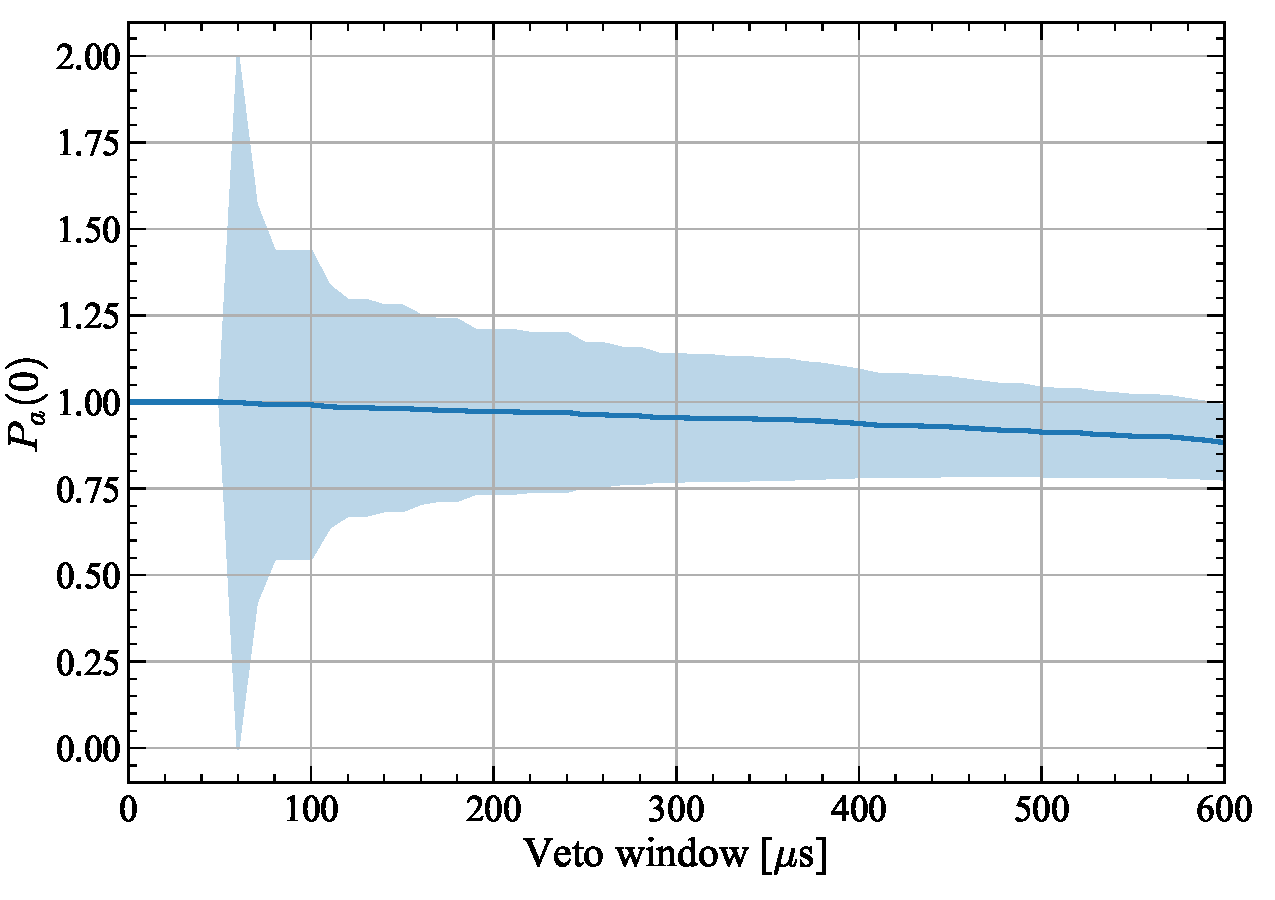
\includegraphics[width=\textwidth]{figures/VetoEfficiency/SR3DDdirect_Corrections_100k.pdf}
        \caption{}
        \label{fig:VetoEff/DDAccCorrectionParameters}
    \end{subfigure}
    \hfill
    \begin{subfigure}[b]{0.49\textwidth}
        \centering
        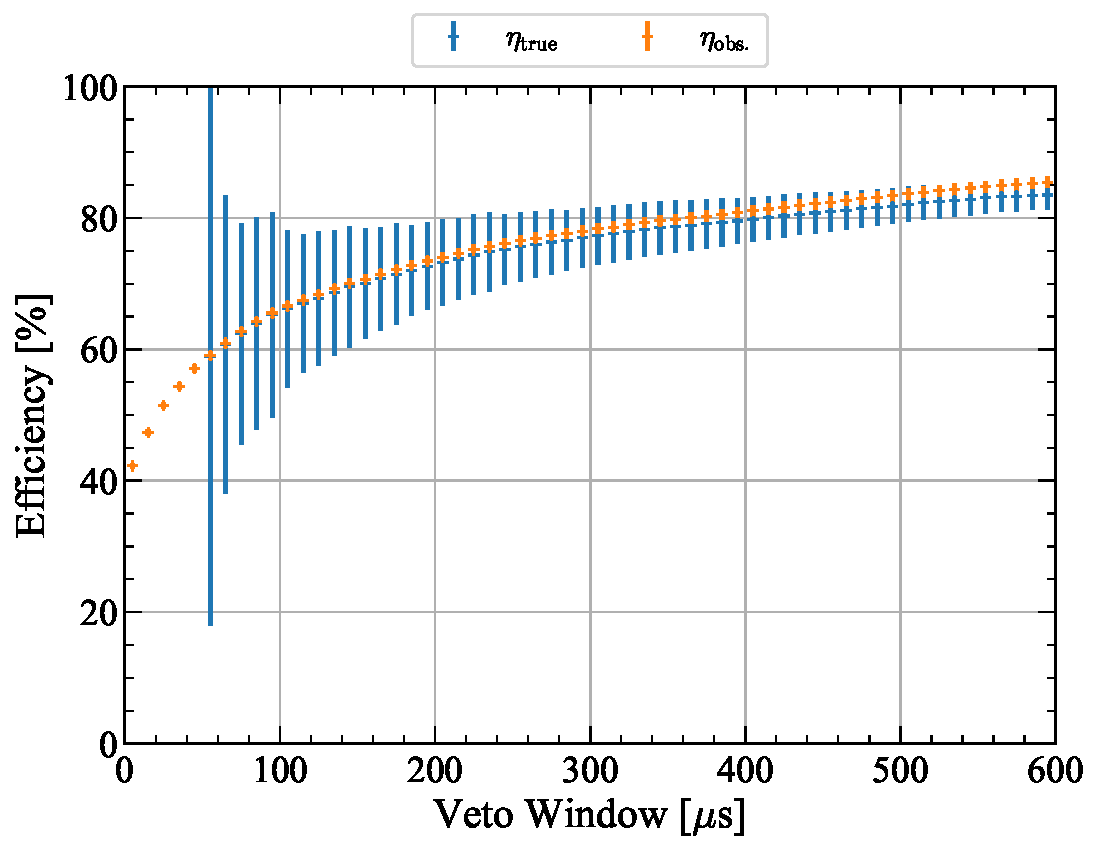
\includegraphics[width=\textwidth]{figures/VetoEfficiency/DDAccidentalCheck.pdf}
        \caption{}
        \label{fig:VetoEff/DDAccCorrectionImpact_P0}
    \end{subfigure}
    \caption[$P(a=0)$ accidental correction factors over a 600~\textmu s for DD calibration sources alongside the veto efficiency with the corrections applied.]{\textbf{Left:} $P(a=0)$ accidental correction factors over a 600~$\mu$s veto window for the DD calibration source data. The errors shown are only statistical uncertainties. The first 60~\textmu s lacks any randomly triggered data to generate accidental corrections during this time. \textbf{Right:} Comparison between calculated veto efficiencies for the DD calibration source with accidental correction applied, $\hat{\eta}$, and not applied, $\eta_\text{obs.}$.}
    \label{fig:VetoEff/DDAccidentalPlots}
\end{figure}

The final efficiencies for DD calibration data corrected for accidental coincidences are shown in \autoref{fig:VetoEff/DDEfficiencies}. At the nominal 600~\textmu s veto window, $\eta^\text{Total}_\text{Data}=(88\pm2)\%$, $\eta^\text{Delayed}_\text{Data}=(84\pm2)\%$, and $\eta^\text{OD Delayed}_\text{Data}=(82\pm3)\%$.

\begin{figure}[h!]
    \centering
    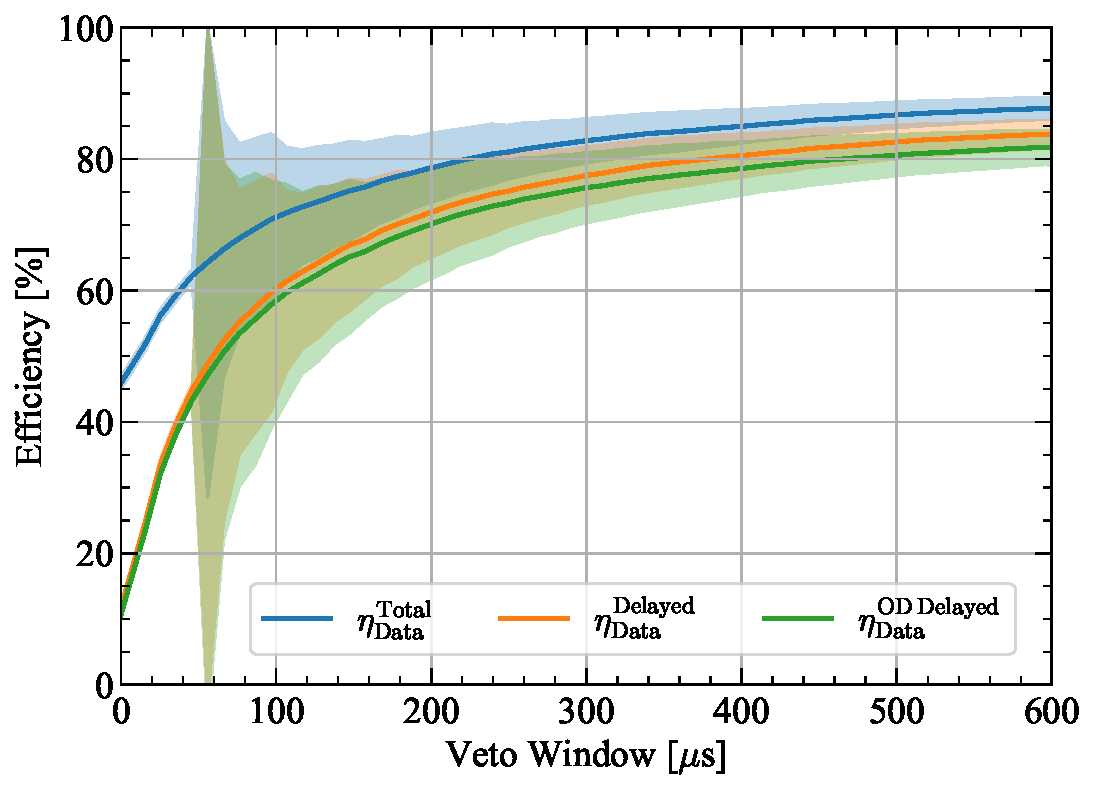
\includegraphics[width=0.7\textwidth]{figures/VetoEfficiency/DDEfficiencies_Data.pdf}
    \caption[DD efficiencies measured in data, all efficiencies are corrected for accidental coincidences.]{DD efficiencies measured in data, all efficiencies are corrected for accidental coincidences. At the nominal 600~\textmu s veto window, $\eta^\text{Total}_\text{Data}=(88\pm2)\%$, $\eta^\text{Delayed}_\text{Data}=(84\pm2)\%$, and $\eta^\text{OD Delayed}_\text{Data}=(82\pm3)\%$.}
    \label{fig:VetoEff/DDEfficiencies}
\end{figure}

\subsection{Simulated neutrons from calibration sources}
AmLi and DD calibration sources are simulated using LZ's \textit{fast} chain simulation technique (discussed in \autoref{sec:LZ/Simulations}). Simulated events which are classified as single scatters by LZLAMA and pass the following selection: S1 and S2 threshold, fiducial volume, CSD selection (AmLi-only, defined in \autoref{eqn:VetoEff/CSDSelection}), and NR Band Selection (defined in \autoref{eqn:VetoEff/NRBandSelection}) are used to determine the calculated veto efficiency (All cuts are defined in \autoref{sec:app/WSCoreCuts} unless stated otherwise.). 
No accidental gammas or neutrons are present in the simulation; therefore, no accidental correction is required. All efficiencies measured using simulated calibration data are presented in \autoref{tab:VetoEff/CalibrationSimulationEfficiencies} and is shown in \autoref{fig:VetoEff/CalibrationSimEfficiencies}.

\begin{figure}[ht!]
    \centering
    \begin{subfigure}[b]{0.49\textwidth}
        \centering
        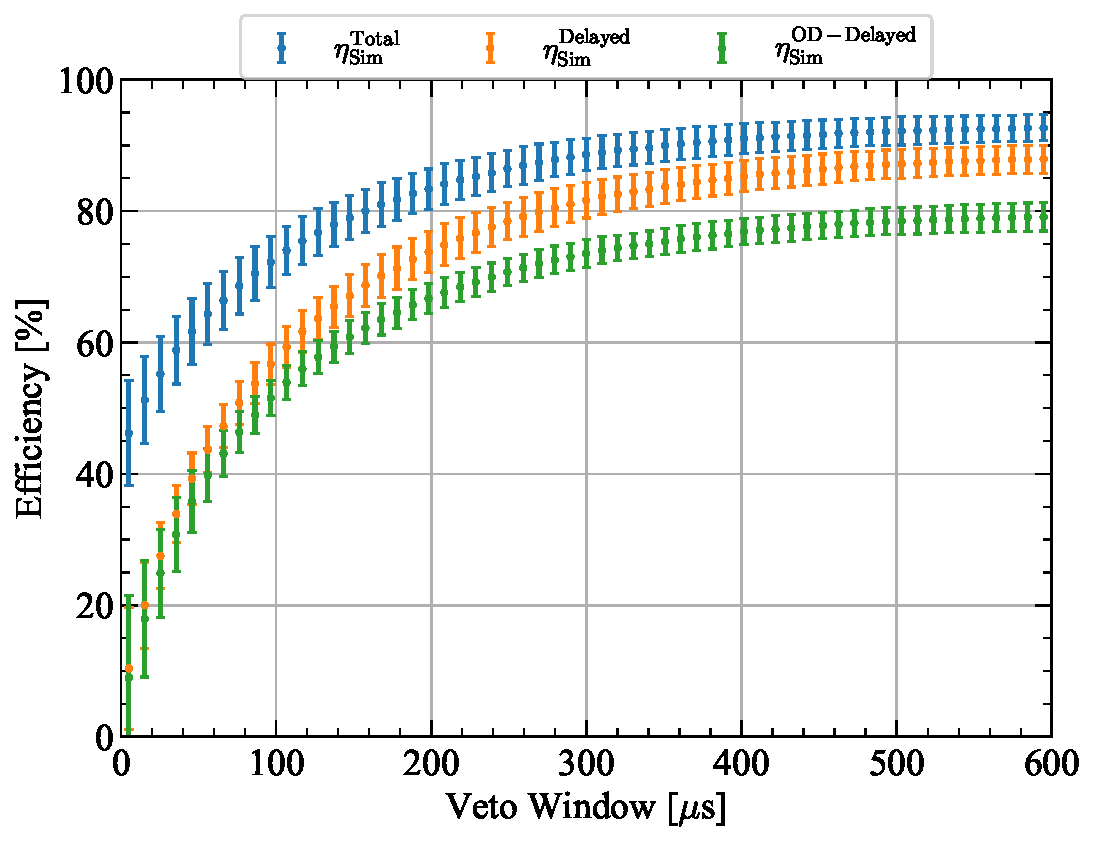
\includegraphics[width=\textwidth]{figures/VetoEfficiency/AmLiEfficiencies_Sim.pdf}
        \caption{}
        \label{fig:VetoEff/AmLiSimEfficiencies}
    \end{subfigure}
    \hfill
    \begin{subfigure}[b]{0.49\textwidth}
        \centering
        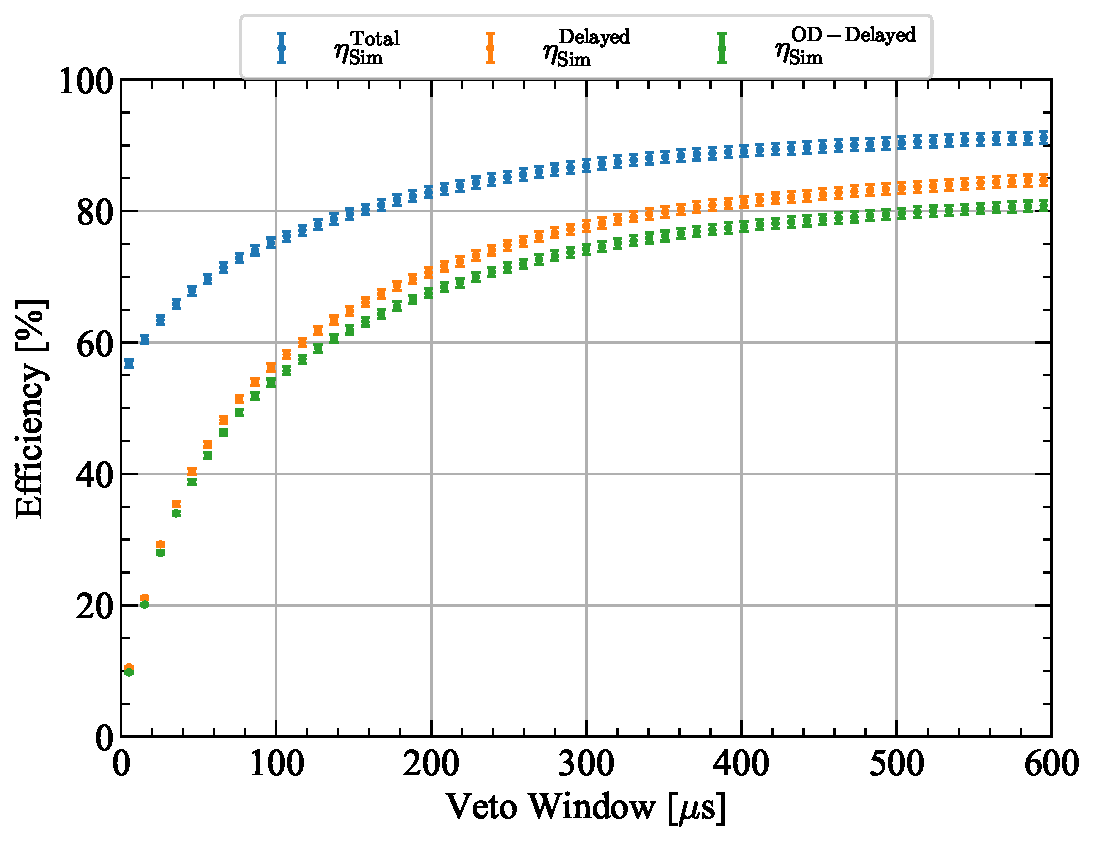
\includegraphics[width=\textwidth]{figures/VetoEfficiency/DDEfficiencies_Sim.pdf}
        \caption{}
        \label{fig:VetoEff/DDSimEfficiencies}
    \end{subfigure}
    \caption[Measured veto efficiencies from AmLi and DD calibration simulations.]{Measured veto efficiencies from AmLi (left) and DD (right) calibration simulations using \textit{Total}, \textit{Delayed}, and \textit{OD Delayed} veto efficiency logic.}
    \label{fig:VetoEff/CalibrationSimEfficiencies}
\end{figure}
\renewcommand{\arraystretch}{1.5}
\begin{table}[h!]
    \centering
    \caption[Calculated efficiencies from AmLi and DD calibration simulations at the nominal 600~\textmu s window.]{Calculated efficiencies from AmLi and DD calibration simulations at the nominal 600~\textmu s window.}
    \begin{tabular}{llll}
    \hline\hline
    \textbf{Source} & \textbf{$\eta^\text{Total}_\text{Sim}$ [\%]} & \textbf{$\eta^\text{Delayed}_\text{Sim}$ [\%]} & \textbf{$\eta^\text{OD Delayed}_\text{Sim}$ [\%]}\\
    \hline
    AmLi & $93\pm2$ & $88\pm3$ & $79\pm3$ \\
    DD & $91\pm1$ & $85\pm1$ & $81\pm1$\\
    \hline\hline
    \end{tabular}
    \label{tab:VetoEff/CalibrationSimulationEfficiencies}
\end{table}
\renewcommand{\arraystretch}{1}

The comparison between veto efficiencies calculated for data and simulation for both sources is shown in \autoref{fig:VetoEff/Sim2DataVetoEffComparisons}. The veto efficiency for AmLi is averaged across all CSD positions and $z$-positions. The percentage difference between the calculated veto efficiency is presented below the veto efficiency curves for both sources. Both sources show agreement when total veto efficiencies are compared with $4\%$ and $2\%$ difference between data and simulation for AmLi and DD calibration sources, respectively.


\begin{figure}[h!]
    \centering
    \begin{subfigure}[b]{0.49\textwidth}
        \centering
        \includegraphics[width=\textwidth]{figures/VetoEfficiency/AmLi_Total_Avg_Ratio.pdf}
        \caption{}
        \label{fig:VetoEff/Sim2DataVetoEffComparisons_AmLi}
    \end{subfigure}
    \hfill
    \begin{subfigure}[b]{0.49\textwidth}
        \centering
        \includegraphics[width=\textwidth]{figures/VetoEfficiency/DDDirect_Total_Ratio.pdf}
        \caption{}
        \label{fig:VetoEff/Sim2DataVetoEffComparisons_DD}
    \end{subfigure}
    \caption[Comparison of calculated data and simulation veto efficiencies for AmLi and DD calibration sources.]{Comparison of calculated data (black) and simulation (red) veto efficiencies for AmLi (left) and DD (right) calibration sources. The difference between the calculated veto efficiency is presented below the veto efficiency curves for both sources. Both sources show good agreement when veto efficiencies are compared with $4.37\%$ and $2.39\%$ difference between data and simulation for AmLi and DD calibration sources, respectively. The lower panel of the DD efficiency comparison has been magnified to better present the difference at 600~\textmu s.}
    \label{fig:VetoEff/Sim2DataVetoEffComparisons}
\end{figure}



\subsection{Background neutrons}\label{sec:VetoEff/BackgroundNeutrons}
Detector NR simulations are produced using LZ's \textit{fast} chain simulation technique as part of the official LZ production before the WS2024 science run.
As part of this production, each of the 644 components that have a radioactive background is simulated.
Simulated events, which are classified as single scatters by LZLAMA and pass the following selection cut: S1 and S2 threshold, fiducial volume, were used to determine the calculated veto efficiency (All cuts are defined in \autoref{sec:app/WSCoreCuts}).
The efficiency of tagging neutrons from Uranium Spontaneous Fission (USF) and ($\alpha$,n) events is shown in \autoref{fig:VetoEff/detector_nr_efficiency}. Also shown is the total efficiency.


\begin{figure}[!ht]
	\centering
	\includegraphics[width=0.7\textwidth]{figures/VetoEfficiency/det_nr_efficiency.png}
	\caption[Efficiencies to veto simulated events which include a single scatter NR TPC.]{Efficiencies to veto simulated events which include a single scatter NR TPC. Each of the 644 background component contributions is weighted according to its contribution to the total NR background. TPC NR events are required to have a reconstructed $z$-position corresponding to an average drift time $t_\text{drift}$ between 350~\textmu s and 700~\textmu s in this example.}
	\label{fig:VetoEff/detector_nr_efficiency}
\end{figure}

\subsection{Background neutron efficiency from data}\label{sec:VetoEff/BkgNeutronEff}
The neutron veto efficiency from each calibration source from data and simulation is shown in \autoref{fig:VetoEff/efficiency_summary}. Also shown is the efficiency from simulated background neutrons.
The $z$-position of each point is calculated from the mean drift time, $\overline{t}_{\text{drift}}$, of events which pass the selection outlined in \autoref{sec:VetoEff/BackgroundNeutrons}.
For the detector NR simulations, the events are separated into three $z$-sections by the following criteria:
\begin{itemize}
    \item \textit{Top:} 71~\textmu s $\leq\overline{t}_{\text{drift}}\leq$350~\textmu s
    \item \textit{Middle:} 350~\textmu s $<\overline{t}_{\text{drift}}\leq$700~\textmu s
    \item \textit{Bottom:} 700~\textmu s $<\overline{t}_{\text{drift}}\leq$1030~\textmu s
\end{itemize}

\begin{figure}[!ht]
	\centering
	\includegraphics[width=0.7\textwidth]{figures/VetoEfficiency/SummaryPlot.pdf}
	\caption[Summary of efficiency from all simulations and calibration sources.]{Summary of efficiency from all simulations and calibration sources. The CSD sources are averaged at each deployment position, $z=100~\text{mm},700~\text{mm},1300~\text{mm}$. Circle markers represent calculated veto efficiencies from data. Star markers represent calculated veto efficiencies from simulation.}
	\label{fig:VetoEff/efficiency_summary}
\end{figure}

Categorisation of detector NR simulation by $t_{\text{drift}}$ is performed to compare the calculated veto efficiencies of the detector NR simulations to veto efficiencies calculated from calibration sources. However, this was not used in the final efficiency evaluation. Shown in \autoref{tab:VetoEff/final_veto_efficiency} are the veto efficiencies of all calibration sources for both simulations and data, alongside the veto efficiencies for the detector NR sources.

The importance of this chapter lies in determining LZ's efficiency to reject background neutrons, the estimated veto efficiency for detector NR events, $\eta_{\text{Det. NR}}^{\text{Data}}$. The method to estimate this efficiency is as follows. 
The average simulation calibration efficiency is taken between, $\overline{\eta}_{\text{AmLi}}^{\text{Sim.}}=(92.8\pm2.0)\%$ and $\eta_{\text{DD}}^{\text{Sim.}}=(91.8\pm1.0)\%$ which results in an average efficiency of $\overline{\eta}_{\text{Cal.}}^{\text{Sim.}}=(92.3\pm1.1)\%$.

The average data calibration efficiency is taken between, $\overline{\eta}_{\text{AmLi}}^{\text{Data}}=(88.6\pm2.7)\%$ and $\eta_{\text{DD}}^{\text{Data}}=(87.7\pm1.8)\%$, which results in an average efficiency of $\overline{\eta}_{\text{Cal.}}^{\text{Data}}=(88.2\pm1.6)\%$.

The difference, $\Lambda$, between the simulation calibration and data calibration efficiencies is used as a systematic uncertainty on the efficiency of detector NR simulations. This process is expressed in \autoref{eqn:VetoEff/DetNR_efficiency}, and produces an estimated veto efficiency for detector NR of $\eta_{\text{Det. NR}}^\text{Data}=(92.2\pm4.3)\%$.

The final uncertainty of the estimated detector NR veto efficiency, $\sigma^\text{Data}_\text{Det. NR}$, is the product of the statistical uncertainty from the simulations $\sigma^\text{Sim.}_\text{Det. NR}=1\%$, and $\Delta=4.2\%$ from the subtraction of the data calibration efficiency from the simulation calibration efficiency.

\begin{equation}
    \label{eqn:VetoEff/DetNR_efficiency}
    \begin{split}
    	\overline{\eta}_{\text{Cal.}}^{\text{Sim.}} & = \frac{\overline{\eta}_{\text{AmLi}}^{\text{Sim.}}+\eta_{\text{DD}}^{\text{Sim.}}}{2}\\
    	\overline{\eta}_{\text{Cal.}}^{\text{Data}} & = \frac{\overline{\eta}_{\text{AmLi}}^{\text{Data}}+\eta_{\text{DD}}^{\text{Data}}}{2} \\
    	\Lambda &= \overline{\eta}_{\text{Cal.}}^{\text{Sim.}} - \overline{\eta}_{\text{Cal.}}^{\text{Data}}\\
    	\eta_\text{Det. NR}^\text{Data}   & = \eta_\text{Det. NR}^\text{Sim.} - \Lambda
    \end{split}
\end{equation}

For the 2024 WIMP search result \cite{LZCollaboration:2024lux}, LZ achieved an estimated neutron tagging efficiency, $\eta_\text{Det. NR}^\text{Data}=(92\pm4)\%$.

\begin{table}[!h]
	\centering
	\caption[Summary of veto tagging efficiencies.]{Summary of veto tagging efficiencies.}
	\begin{tabular}{lll}
    \hline\hline
    \textbf{Source}& \textbf{$\eta^\text{Sim.}$ [\%]}& \textbf{$\eta^\text{Data}$ [\%]}\\ 
    \hline
    AmLi (average) & 92.8$\pm$2.0 & 88.6$\pm$2.7\\
    DD & 91.8$\pm$1.0 & 87.7$\pm$1.8\\
    Sources (average)& $92.3\pm1.1$ & $88.2\pm1.6$\\
    Detector NR & 96.4$\pm$1.0 & 92.2$\pm$4.3\\
    \hline\hline
	\end{tabular}
	\label{tab:VetoEff/final_veto_efficiency}
\end{table}

\newpage

\section{Veto selection and the 2024 WIMP search result}\label{sec:VetoEff4WIMPSearch}
Candidate events for the WIMP search analysis (see \autoref{chap:WS2024Result}) are selected using a series of event and data selections. The cuts described in the \autoref{sec:VetoEff/VetoSelectionOptimisation} are the ``veto coincidence cuts'' which are used to reject SS events that are accompanied by a coincident signal in the Skin and/or OD. The greatest benefit of the veto system to the WIMP search analysis is the increase in the fiducial volume of the TPC. Background events produced near the walls of the TPC are tagged by the veto system and are rejected from the analysis. In the absence of the veto system, the optimum method of removing background events near the wall would be to remove that portion of the target mass entirely. This method would result in a 40\% decrease in exposure \cite{lkorley:thesis}. This is not a suitable method for a dark matter direct detection search, where the amount of target mass should be maximized, where possible. The reconstructed TPC position of events selected by the veto coincidence cuts is shown in \autoref{fig:VetoEff/WS2024_TPCPosPlots_2panel} alongside candidate events used for the 2024 WIMP search analysis.
\begin{figure}[h!]
    \centering
    \includegraphics[width=\linewidth]{figures/VetoEfficiency/WS2024_TPCPosPlots_2panel.png}
    \caption[Data from the WS2024 science run reconstructed in TPC with events that are vetoed coloured in red and blue.]{\textbf{Left:} Data from the WS2024 science run reconstructed in TPC $x$ and $y$ position, in black with all analysis cuts applied. Red crosses and blue circles represent events that are vetoed by the Skin and OD veto coincidence cuts, respectively. The dashed line shows the active volume, averaged over azimuth, and the solid lines depict the FV at the azimuths of its smallest and largest radial extent. The two circle lines depict the boundary of the position-based selection, which removes events within 6~cm of TPC field cage resistors with elevated rates of radioactivity. \textbf{Right:} The same events shown in the left panel are reconstructed in TPC $\text{R}^2$ and $z$.}
    \label{fig:VetoEff/WS2024_TPCPosPlots_2panel}
\end{figure}

Events that have a coincidence signal in the delayed veto window have a higher chance of having been caused by a neutron recoiling in the TPC. Selecting events with a veto signal, therefore, yields a neutron-rich sideband with which we constrain the neutron rate in the WIMP 2024 data set.
Events that passed the Skin-delayed and OD-delayed selection are used to generate the sideband sample. In the final statistical analysis, a likelihood fit returns an expectation of $0.0^{+0.2}$ SS counts attributed to detector neutrons \cite{LZCollaboration:2024lux}. The events selected for this sideband analysis are shown in \autoref{fig:VetoEff/VetoSideBandEvents} and are overlaid against the final set of events passing all selection cuts. 

\begin{figure}[h!]
    \centering
    \includegraphics[width=0.7\linewidth]{figures/VetoEfficiency/WS2024VetoSideBandEvents_WIMP40.png}
    \caption[Final set of events passing all selection cuts in the WS2024 dataset with events tagged by the OD and Skin overlaid.]{The final set of events passing all selection cuts is shown in black. Events that are tagged by the Skin and OD delayed selection are shown in red. Regions containing 68\% and 95\% of the ER portion of the background model and a 40~GeV/$c^2$ WIMP are shown with the dark and light gray and purple shading, respectively. Gray lines show contours of constant ER-equivalent ($\text{keV}_\text{ee}$) and NR-equivalent ($\text{keV}_\text{nr}$) energy. The dashed lines show the boundary of the WIMP region of interest.}
    \label{fig:VetoEff/VetoSideBandEvents}
\end{figure}

\pagebreak

\section{Concluding remarks}
Improvements to the Outer Detector geometry in simulation now better reflect the neutron capture timing observed in calibration data sets. As the time between single scatter S1 and veto pulses is considered in the veto coincidence selection, the accurate modelling of the detector response in simulation is crucial for the optimisation of veto coincidence selection for the WIMP analysis. These improvements are further reflected in the measurement of the neutron tagging efficiency when results are compared to simulations of AmLi and DD calibration sources. The optimisation of the veto coincidence selection resulted in a factor of two reduction in detector dead time induced by the selection whilst maintaining the same tagging efficiency measured in the WS2022 science run. An estimated neutron tagging efficiency of $(92\pm4)\%$ with a 3\% detector dead time is presented. The inclusion of the veto coincidence selection to the WIMP analysis cuts affords LZ the ability to increase the fiducial volume by 40\% by rejecting background events near the wall of the TPC, which otherwise would be removed by constraining the fiducial volume selection. To estimate the number of single scatter events resulting from detector neutrons, a sample data set of events selected using the delayed veto coincidence selection is generated. An expectation of $0.0^{+0.2}$ single scatter events is attributed to detector neutrons using likelihood fit analysis. It should be stressed that if a WIMP signal were observed by LZ, the veto system will be crucial to exclude backgrounds as an explanation for the excess. To conclude this chapter, I echo the words of Carl Sagan, \textit{``extraordinary claims require extraordinary evidence''} \cite{SaganCarl:BrocasBrain}.
\chapter{Atmospheric muons and the LUX-ZEPLIN experiment}\label{chap:Muons}
Atmospheric muons pose a threat to direct detection dark matter searches such as LZ. Energetic neutrons which could mimic a dark matter signal can be produced through muon interactions with detector and the surrounding materials \cite{LZ_SIMS}. To decrease the impact that atmospheric muons have on rare event searches, experiments are situated at deep underground sites. 
The production mechanisms for atmospheric muons from cosmic rays and how the intensity of the muon flux varies between the Earth's surface and at underground sites is first discussed in \autoref{sec:Muons/CosmicRays} and \autoref{sec:Muons/MuonsUnderground}. How muons interact as they travel through materials and the induced backgrounds from such interactions is discussed in \autoref{sec:Muons/MuonTransport} and \autoref{sec:Muons/InducedBackgrounds}. The measurement of the muon flux through the LZ experiment is presented in \autoref{sec:Muons/MuonFluxMeasurementWithLZ} alongside the impact that muons have on the WIMP and the measures taken to veto muons events and the additional aftermath left in the detector after a muon has travelled through is discussed in \autoref{sec:Muons/MuonVeto}. How the muon flux in LZ modulates over time is discussed in \autoref{sec:Muons/MuonModulation}.

\section{Cosmic rays and atmospheric muons}\label{sec:Muons/CosmicRays}
Atmospheric showers are produced from the collision of primary cosmic radiation with the upper Earth's atmosphere. Primary cosmic radiation can be attributed to a non-thermal population of particles that pervade the Universe \cite{ParticleDataGroup:2024cfk}. The charged cosmic rays (CRs) consist mostly of nuclei and electrons at a ratio of 49:1, where the majority of the nuclei are Hydrogen (87\%) and Helium (12\%) with 1\% in the form of heavier elements \cite{Longair_2011}. The energy spectrum of primary CRs can be described using the following power law:
\begin{equation}\label{eqn:Muons/CREnergy}
    \frac{E^2dJ}{dE}\sim E^{-\gamma},
\end{equation}
where the spectral index, $\gamma$, varying across the energy spectrum in the range of $2.5\lesssim\gamma\lesssim3$ \cite{ParticleDataGroup:2024cfk}. Charged CRs follow a power law with a spectral index $\gamma\simeq2.7$ for energies up to a few PeV. The combined energy spectra for charged CRs, gamma-rays and neutrinos is shown in \autoref{fig:Muons/CREnergySpec}.
\begin{figure}[ht!]
    \centering
    \includegraphics[width=0.7\linewidth]{figures/Muons/CosmicRaySpectra.png}
    \caption{The spectrum of cosmic rays (CRs), diffuse gamma-rays and neutrinos. The measurements of intensity of charged and neutral CRs multiplied by the kinetic energy squared. Energy-integrated intensities are shown by the various diagonal lines. Figure reprinted from Ref.~\cite{ParticleDataGroup:2024cfk}.}
    \label{fig:Muons/CREnergySpec}
\end{figure}
A number of secondary particles are produced through CR interactions with atmospheric nuclei. For high energy protons ($\geq 1~\text{GeV}$), the de Broglie wavelength of the incident particle is much less than the distance between nucleons in the nucleus \cite{Longair_2011}. Therefore the proton can interact with individual nucleons within the nucleus. In such collisions, pions of all charges, $\pi^+,\:\pi^-\text{, and }\pi^0$ are the principle products. In additions to these mesons, the nucleons involved in the interaction may also be expelled from the nucleus. This results in the nucleus being left in a highly unstable excited state that ejects several nuclear fragments in the form of other light nuclei, protons and/or neutrons. These are called spallation fragments. Further reactions in the form of nucleonic cascades are induced by these products, as well as pions, kaons and other mesons.

Nucleons and charged pions with sufficient energy will continue to multiply in successive collisions until the energy per particle drops below the threshold required for multiple pion productions, also known as \textit{hadronisation} \cite{Longair_2011}. Pions have very short lifetimes and decay. Neutral pions decay to two $\gamma$-rays ($\pi^0\rightarrow2\gamma$), which initiate electromagnetic cascades through the conversion into an electron-positron pair ($\gamma\rightarrow e^-+e^+$). The electromagnetic shower is formed through the continued succession of pair production and bremsstrahlung processes. Charged pions decay into muons through the following reactions:
\begin{equation}
\begin{split}
    \pi^+&\rightarrow\mu^++\nu_\mu \\
    \pi^-&\rightarrow\mu^-+\bar\nu_\mu
\end{split}
\end{equation}
Other mesons, such as kaons, have analogous decay processes. Very high energy muons are produced in the uppermost layers of atmosphere before the pions make further nuclear interaction. 
%Muons have virtually no nuclear interactions and are very penetrating. 
In the rest frame of the muon, they decay with a mean lifetime of $2.2\times10^{-6}~\text{s}$. However, to an external observer they decay with an observed lifetime of $2.2\times10^{-6}\gamma~\text{s}$ due to relativistic time dilation where $\gamma$ is the Lorentz factor. At high energies, the incoming muons have Lorentz factors $\gamma\geq20$ resulting in a time dilation and length contraction which enables them to reach the Earth's surface. 

Lower energy muons have time to decay in-flight into electrons, positrons, and neutrinos that can go on to produce further low-energy electromagnetic showers:
\begin{equation}
\begin{split}    
    \mu^+&\rightarrow e^++\nu_e+\bar\nu_\mu \\
    \mu^-&\rightarrow e^-+\bar\nu_e+\nu_\mu
\end{split}
\end{equation}
The interaction of a primary cosmic ray in the atmosphere and the subsequent interactions of the products from the nucleonic cascades are depicted in a diagram shown in \autoref{fig:Muons/CRDiagram}.
\begin{figure}[ht!]
    \centering
    \includegraphics[width=0.7\linewidth]{figures/Muons/MuonShower.png}
    \caption{Diagram showing the interaction of a primary cosmic ray with nuclei in the upper Earth's atmosphere and the development of a nucleon cascade producing secondary cosmic rays in the form of muons, neutrinos and electromagnetic showers. Figure reprinted from Ref.~\cite{Longair_2011}.}
    \label{fig:Muons/CRDiagram}
\end{figure}
As shown in \autoref{eqn:Muons/CREnergy}, the primary CR spectrum follows a power-law which is consequently applicable to the secondary CR products. However, the muon spectrum has added complexity as charged mesons interact with the atmosphere and in turn lose energy before decaying. T.K. Gassier proposed a parametrisation \cite{Gaisser_Engel_Resconi_2016} which results in an approximate formula for the muon spectrum at sea level:
\begin{equation}
    \label{eqn:Muons/MuonIntensitySurfaceEarth1}
    \frac{dI_\mu}{dE_{\mu0}d\Omega}\approx\frac{0.14\times E^{-\gamma}_{\mu0}}{\text{cm}^2\cdot\text{s}\cdot\text{sr}\cdot\text{GeV}}\times\Biggl\{\frac{1}{1+\frac{1.1\:E_{\mu0}\text{cos}\theta}{115\text{ GeV}}}+\frac{0.054}{1+\frac{1.1\:E_{\mu0}\text{cos}\theta}{850\text{ GeV}}}\Biggl\},
\end{equation}
where $\frac{dI_\mu}{dE_{\mu0}d\Omega}$ is the differential muon intensity at sea level, $E_{\mu0}$ is the muon energy at the Earth's surface and $\theta$ is the zenith angle of the muon at the surface (valid for $\theta<70^\circ$, accounting for the curvature of Earth). A spectral index, $\gamma=2.7$ was proposed by Gaisser \cite{Gaisser_Engel_Resconi_2016}. The two terms within the parentheses represent the muon produced from pion decay and kaon decay respectively, where the values of 115~GeV and 850~GeV correspond to the critical energies of these two particles. The critical energy is defined as the energy at which the probability of interaction is equal to the probability of decay at the height of a decay. There is an angular dependence of this term because high energy pions will traverse less atmosphere before decaying into a high energy muon.
Taking into account the curvature of Earth and additional muon processes, \autoref{eqn:Muons/MuonIntensitySurfaceEarth1} is modified as follows:
\begin{equation}
\label{eqn:Muons/MuonIntensitySurfaceEarth2}
\begin{split}    
    \frac{dI_\mu}{dE_{\mu0}d\Omega}(E_{\mu0},\theta^*)\approx&\frac{A\times 0.14\times (E_{\mu0}+\Delta E_{\mu0})^{-\gamma}}{\text{cm}^2\cdot\text{s}\cdot\text{sr}\cdot\text{GeV}}\\
    &\times\Biggl\{\frac{1}{1+\frac{1.1\:(E_{\mu0}+\Delta E_{\mu0})\text{cos}\theta_1}{115\text{ GeV}}}+\frac{0.054}{1+\frac{1.1\:(E_{\mu0}+\Delta E_{\mu0})\text{cos}\theta_1}{850\text{ GeV}}}+R_c\Biggl\}\times p_d,
\end{split}
\end{equation}
where $\frac{dI_\mu}{dE_{\mu0}d\Omega}(E_{\mu0},\theta^*)$ is the differential muon intensity at sea level, $\theta_1$ is the zenith angle at production of site of the muon in the atmosphere which relates to $\theta^*$ as follows, $\text{cos}\:\theta_1=\sqrt{1-0.99\cdot(1-\text{cos}^2\:\theta^*)}$, $\Delta E_{\mu0}$ is the muon energy loss in the atmosphere, $R_c=1\times10^{-4}$ is the ratio of muons to pions \cite{LVD:1998lir}, and $p_d$ is the probability for the muon not to decay in the atmosphere. The survival probability for high energy muons which reach deep underground labs is practically 1, so the precise parametrisation of the muon decay probability is not critical for underground muon physics.

The normalisation factor $A$ and the spectra index $\gamma$ can be chosen to fit experimental data and is dependent on depth. For depths $>2.5~\text{km}$ water equivalent (w.e.), the relation for `depth - vertical muon intensity' measured by the LVD experiment found $\gamma=2.77$ with a normalisation of the absolute flux $A=1.84$ found a good fit to data \cite{LVD:1998lir}.

\section{Muon transport through materials}\label{sec:Muons/MuonTransport}
As muons are charge particles they lose energy as they traverse materials through electromagnetic interactions with nuclei and atomic electrons in the medium. Energy loss through ionisation is the process where the passing charged particle (a muon in this particular case) transfers energy to the atomic electrons. The atom will either be excited or ionised depending on the proximity of the charged particle. The mean rate of energy loss of a muon due to ionisation and excitation can be described using the Bethe-Bloch formula:
\iffalse
\begin{equation}\label{eqn:Muons/BetheBloch}
    -\Biggl<\frac{dE}{dx}\Biggl>=4\pi\alpha^2N_A\frac{Z}{A}\frac{z^2(\hbar c)^2}{m_e^2v^2}\Biggl[\text{ln}\frac{2m_ev^2\gamma^2}{I}-\frac{v^2}{c^2}-\delta(\beta\gamma)\Biggl],
\end{equation}
\fi

\begin{equation}\label{eqn:Muons/BetheBloch}
    -\Biggl<\frac{dE}{dx}\Biggl>=Kz^2\frac{Z}{A}\frac{1}{\beta^2}\Biggl[ \frac{1}{2}\text{ln}\frac{2m_ec^2\beta^2\gamma^2T_{\text{max}}}{I^2}-\beta^2-\frac{\delta(\beta\gamma)}{2}\Biggl],
\end{equation}
where $K=4\pi N_\text{A}r_e^2m_ec^2$, $T_{\text{max}}=2m_ec^2\beta^2\gamma^2/(1+2\gamma m_e/m_\mu+(m_e/m_\mu)^2)$ which is the maximum energy transfer in a single collision, $z$ is the charge of the muon (in units of electric charge), $\gamma=1/\sqrt{1-\frac{v^2}{c^2}}$ is the Lorentz factor, $v$ is the velocity of the muon with mass $m_\mu$ and energy $E$, $I\simeq16\:\cdot\:Z^{0.9}$ eV is the mean ionisation potential of the atom \cite{GROOM2001183}. As the energy of the muon increases, the inelastic cross-section increases, increasing the number of interactions with distant electrons. This effect is corrected for in \autoref{eqn:Muons/BetheBloch} by the density correction term $\delta(\beta\gamma)$.

Muons additionally lose energy through radiative processes, which occur as discrete events involving large energy losses, in contrast to the smaller but continuous energy losses from ionisation. The total mean energy loss of the muon can be described as:
\begin{equation}\label{eqn:Muons/totMeanEnergyLossMu}
    \Biggl<-\frac{dE}{dx}\Biggl>=a(E)+b(E)E,
\end{equation}
where $x$ is the path length, $a(E)$ is the energy loss through ionisation as described with \autoref{eqn:Muons/BetheBloch}, and $b(E)$ is due to radiative
processes — bremsstrahlung, pair production, and photonuclear interactions:
\begin{equation}\label{eqn:Muons/radproc}
    b\equiv b_{\text{brems}}+b_{\text{pair}}+b_{\text{nucl}},
\end{equation}
where these three stochastic energy-loss processes with respect to charged particle are described briefly below:
\begin{itemize}
    \item \textbf{Bremsstrahlung:} As a charge particle passes near to the nucleus it decelerates, radiating a photon.
    \item \textbf{Pair-production:} Charged particles interact via the electromagnetic force, this interaction is mediated by a virtual photon, which in the field of the nucleus converts into a electron-positron pair.
    \item \textbf{Photonuclear interaction:} A photon radiated by the charged particle is absorbed by the nucleus and enters an excited state. The nucleus immediately decay releasing a hadron.
\end{itemize}
Both $a(E)$ and $b(E)$ are slowly varying functions of $E$, where at high energies losses by radiative processes dominate. The contributions from ionisation and radiative processes to the total stopping power of muons on copper is shown in \autoref{fig:Muons/StoppingPowerOffMuonsCu}. The critical energy, $E_{\mu c}$, is the energy at which the losses from ionisation and radiative processes are equal and is dependent on the material which the muon is propagating through.
\begin{figure}
    \centering
    \includegraphics[width=0.7\linewidth]{figures/Muons/MassMuonStoppingPowerOfMuonsOnCu.png}
    \caption{Mass stopping power $\big<-dE/dx\big>$ for positive muons on copper as a function of $p=M\beta c\gamma$. Figure reprinted from Ref.~\cite{GROOM2001183}.}
    \label{fig:Muons/StoppingPowerOffMuonsCu}
\end{figure}
In addition to the discussed energy loss processes, muons will also elastically scatter from nuclei via Coulomb interactions. However, the energy loss from this type of scattering can be consider negligible. As the muon propagates through a material, it will deviate from its track due to small angle deviations from the collective Coulomb scatters. 

\section{Muons underground}\label{sec:Muons/MuonsUnderground}
As a muon travels to from the surface to an underground site, the muon will undergo energy losses, as discussed in \autoref{sec:Muons/MuonTransport}. Depending on the energy of the incoming muon, it will either decay, be absorbed by the rock overburden, or reach the underground site. Due to this effect, muon intensity underground decreases with depth.

The muon spectrum underground can be described by \autoref{eqn:Muons/MuonIntensityUnderground}, which the convolution of the spectrum on the surface, (\autoref{eqn:Muons/MuonIntensitySurfaceEarth2}, and the probability for a muon with energy $E_{\mu 0}$ at the surface to have the energy $E_\mu$ at a depth $X$ \cite{musun}.
\begin{equation}\label{eqn:Muons/MuonIntensityUnderground}
    \frac{dI_\mu}{dE_\mu d\Omega}(dE_\mu d\theta)=\int^\infty_0P(E_\mu,X(\theta),E_{\mu0})\frac{dI_{\mu0}}{dE_{\mu0}d\Omega}(E_{\mu0},\theta^*)dE_{\mu 0}
\end{equation}
Simulation packages have been developed to model the passage of muons through large thicknesses of material to determine $P(E_\mu,X(\theta),E_{\mu0})$, one example which has been adopted by LZ is MUSIC (\textbf{MU}on \textbf{SI}mulation \textbf{C}ode) which has been extensively tested against experimental data and other packages \cite{musun,LVD:1998lir,PhysRevD.60.112001,Tang:2006uu,MACRO:2003qix}. The use of MUSIC alongside MUSUN (\textbf{MU}on \textbf{S}imulations \textbf{UN}derground) for muon simulations for LZ will be discussed in \autoref{sec:Muons/MuonFluxMeasurementWithLZ}.
The dependence of vertical muon intensity on depth for both water and rock is shown in \autoref{fig:Muons/MuonIntensityVSDepth}. Additional data on the total muon flux at various underground sites for equivalent depth relative to a flat overburden is summarized in \autoref{tab:Muons/MuonFluxVsDepth} and shown in \autoref{fig:Muons/MuonFluxVsDepth}.
\begin{figure}[ht!]
    \centering
    \includegraphics[width=0.7\linewidth]{figures/Muons/MuonIntensityVSVertDepth.png}
    \caption{Vertical muon intensity dependence on depth for standard rock ($\langle Z\rangle=11$) and water. The filled triangles correspond to a collection of experiments with a rock overburden \cite{Kozyarivsky:1988gxn}. The open circles are data points taken the Baikal underwater neutrino telescope \cite{BAIKAL:1997iok}. Figured reprinted from Ref.~\cite{dwoodward:thesis}.}
    \label{fig:Muons/MuonIntensityVSDepth}
\end{figure}
\begin{figure}[ht!]
    \centering
    \includegraphics[width=0.7\linewidth]{figures/Muons/Flux_Depth_Plot.pdf}
    \caption{The total muon flux measured for different underground sites summarised in \autoref{tab:Muons/MuonFluxVsDepth} as a function of equivalent vertical depth relative to a flat overburden. The smooth curve is global fit function is described in Ref.~\cite{mei}. Plot adapted from Ref.~\cite{mei}.}
    \label{fig:Muons/MuonFluxVsDepth}
\end{figure}

\begin{table}[ht!]
    \centering
    \caption{Summary of the total muon flux measured at different underground sites and the equivalent vertical depth relative to a flat overburden ($^\dagger$Equivalent vertical depth with flat overburden). Adapted from Ref.~\cite{mei}.}
    \label{tab:Muons/MuonFluxVsDepth}
    \begin{tabular}{lll}
        \hline\hline
        \textbf{Laboratory} & \textbf{Muon flux [$\text{cm}^{-2}\text{s}^{-1}$]}&\textbf{Depth [km]}\\
        \hline
        WIPP & $(4.77 \pm 0.09) \times 10^{-7}$ & $1.59 \pm 0.01$ \\
        Soudan & $(2.00 \pm 0.20) \times 10^{-7}$ & $1.95 \pm 0.15$ \\
        Kamioka$^\dagger$ & $(1.58 \pm 0.21) \times 10^{-7}$ & $2.05 \pm 0.15$ \\
        Boulby & $(4.09 \pm 0.15) \times 10^{-8}$ & $2.81 \pm 0.02$ \\
        Gran Sasso$^\dagger$& $(2.78 \pm 0.20) \times 10^{-8}$ & $3.05 \pm 0.20$ \\
        Fréjus$^\dagger$ & $(5.47 \pm 0.10) \times 10^{-9}$ & $4.15 \pm 0.20$ \\
        Homestake & $(5.31 \pm 0.17) \times 10^{-9}$ & $4.30 \pm 0.20$ \\
        Sudbury & $(3.77 \pm 0.41) \times 10^{-10}$ & $6.01 \pm 0.10$ \\
        \hline\hline
    \end{tabular}
\end{table}

\section{Muon induced backgrounds}\label{sec:Muons/InducedBackgrounds}
Atmospheric muons which reach underground sites and traverse through a detector are detected as background events in the case of dark matter direct detection experiments. However, high-energy muons can be problematic to rare event searches since they produce secondary particles due to interactions with the rock overburden close to the detector and other material within and surrounding the detector. Muons which miss the detector but produce associated secondary particles may produce signal-like events. These such events cannot be rejected through coincidence with the incident muon \cite{mei,Lindote:2008nq}. Muon-induced neutrons, one such secondary particle, are particularly troublesome for dark matter detectors which cannot discriminate between single neutron interactions and dark matter candidates. The contribution of muon-induced neutrons to the total underground neutron flux in small \cite{LZ_SIMS}, however muon-induced neutrons have an energy spectrum up to several GeV. Fast neutrons with such energies are impervious to passive detector shield and interact with the detector. There are several processes which produce neutrons from high-energy muons:
\begin{equation}\label{eqn:Muons/MuonInt1}
    \mu^-+X\rightarrow X' + n+\nu_\mu
\end{equation}
\begin{equation}\label{eqn:Muons/MuonInt2}
    \mu^-+p\rightarrow n+\nu_\mu
\end{equation}
\begin{equation}\label{eqn:Muons/MuonInt3}
    \gamma+X\rightarrow X'+n
\end{equation}
\begin{equation}\label{eqn:Muons/MuonInt4}
    \pi+X\rightarrow X'+n
\end{equation} 
where $X$ and $X'$ represent the initial and final states of nuclei. \autoref{eqn:Muons/MuonInt1} represents neutron production via nuclear interactions caused directly by the muons through spallation. \autoref{eqn:Muons/MuonInt2} represents negative muon capture on a proton in the nucleus of the target atom. \autoref{eqn:Muons/MuonInt3} and \autoref{eqn:Muons/MuonInt4} represent products of muon-induced electromagnetic or hadronic cascades interacting with the nucleus of the target atom.
%The contribution of negative muon capture to the muon-induced neutron flux depends on the ratio of stopping-muons to through-going muons.
The contribution of negative muon capture (\autoref{eqn:Muons/MuonInt2}) to the muon-induced neutron flux is dependent on the ratio of stopping-muons to through-going muons. The rate of stopping-muons is energy dependent of incoming atmospheric muons due to the loss of momentum whilst travelling through rock and the production of secondary particles which the mechanisms discussed in \autoref{sec:Muons/MuonTransport}. Thus the rate of negative muon capture is only significant at depths $\lesssim100~\text{m w.e.}$ \cite{Gaisser_Engel_Resconi_2016}. The rate of neutron production from electromagnetic and hadronic cascades is significantly larger than the rate of neutron production via muon-induced spallation at deep underground sites.

In general, the rate of muon-induced backgrounds is dependent on two factors, the depth of the underground site and the composition of the overburden material. To understand the effect that muon-induced background have on deep underground detectors, an initial measurement of the muon flux through the detector in question must be made. The following sections discuss the muon flux measurement with the LZ experiment, modulation of the muon flux and their direct impact on data taking during the WS2022 and WS2024 WIMP search campaigns.  

\section{Muon flux measurement with the LUX-ZEPLIN experiment}\label{sec:Muons/MuonFluxMeasurementWithLZ}
The initial muon model adapted by LZ described in Ref.~\cite{LZ_SIMS} is used to calculate muon fluxes that can be compared with previous measurements. Vertical muon intensity is calculated as $5.18\times10^{-9}$~cm$^{-2}$~s$^{-1}$~sr$^{-1}$, in good agreement with the value of $(5.38\pm0.07\text{ (stat)})\times10^{-9}$~cm$^{-2}$~s$^{-1}$~sr$^{-1}$~\cite{Cherry} measured in the same cavern using the veto system of the Davis experiment. Total muon flux through a hypothetical spherical detector with unit cross-sectional area is calculated as $6.16\times10^{-9}$~cm$^{-2}$~s$^{-1}$, slightly higher than the measurements with the veto system of the Majorana Demonstrator located in the nearby cavern $(5.31\pm0.17 \text{ (stat)})\times10^{-9}$~cm$^{-2}$~s$^{-1}$~\cite{majorana}.
The difference between the two measurements and the initial model, although relatively small within $20\%$, motivates a need for new measurements with the LZ experiment to re-normalise the muon model. The new muon flux measurements estimate the average density of the rock between the surface and the cavern and will be used to inform the muon model for the DUNE experiment\cite{DUNE}, which uses the same simulation code and the same rock density.

\subsection{Outline of model}\label{sec:Muons/ModelOutline}
The muon simulations use two Monte-Carlo codes: MUSIC and MUSUN, adapted here for the LZ experiment. Initially, muons with different energies on the surface of the Earth are transported through various distances in rock using MUSIC. The rock composition is taken from Ref.~\cite{mei,zhang}. Measurements of several rock samples have been reported~\cite{mei,zhang} and the average rock parameters have been calculated as $\langle Z\rangle=12.09$ and $\langle A\rangle=24.17$. The average density of rock is assumed to be $2.70~\text{g/cm}^3$~\cite{zhang} in the MUSIC simulation. Other measurements \cite{Heise:2021eym}, including the measurement of the muon flux with the veto system of the Majorana demonstrator, suggest that the density may be larger ($2.8-2.9~\text{g/cm}^3$\cite{majorana}).

The resulting energy spectra of surviving muons is convoluted with muon spectra on the surface of the Earth for different zenith angles and slant depths, see Ref.~\cite{musun}. The distance from the underground laboratory and the Earth's surface for each azimuth and zenith angle is obtained from the surface map and the position of the laboratory in the global coordinate system \cite{richardson}.
Muon energy spectrum and zenith angle distribution on the surface of the Earth are calculated using \autoref{eqn:Muons/MuonIntensitySurfaceEarth2} modified for the curvature of the Earth to include large zenith angles. Other corrections, such as muon decay and energy loss in the atmosphere, muon production via charmed meson decay, muon intensity dependence on altitude and geomagnetic rigidity cut-off are not included due to their negligible effect on high-energy muons (\textgreater~1~TeV) capable of reaching the Davis Cavern.
As a result of muon transport and convolution with the surface fluxes, muon energy spectra and different angles at the detector site are calculated and stored. The model gives the total muon flux through a sphere as $6.16\times10^{-9}$~cm$^{-2}$~s$^{-1}$, mean muon energy of 283~GeV, mean zenith angle of 27$^{\circ}$ and the mean slant depth of 4500~m~w.e.~\cite{musun-lz}.

The muon generator, MUSUN, inside BACCARAT reads muon distributions from the MUSIC output and samples muons on the horizontal (top) and vertical surfaces of a rectangular volume that encompasses the laboratory hall. The top horizontal surface of the volume is located 7~m above the cavern boundary. Vertical surfaces of the volume are positioned 5~m away from the boundary. The volume extends to 3~m below the cavern floor. Moving the volume surfaces into the rock, away from the cavern, ensures the development of muon-induced cascades in rock or shotcrete before muons and their secondaries enter the cavern. The primary energy spectrum and the angular distributions of these muons as well as the surface topography are shown in \autoref{fig:Muons/Prime_info}. The GEANT4 {\fontfamily{qcr}\selectfont G4GeneralParticleSource} function is used to generate the muons, and their charge is based on the output sampled from MUSIC. The ratio of $\mu+/\mu-$ is set to 1.38 based on measurements of high energy muons \cite{Ashley:1975uj}.
\begin{figure*}[ht!]
    \centering
    \begin{subfigure}[b]{0.48\textwidth}
        \centering
        \includegraphics[width=\textwidth]{figures/Muons/Primary_energyLZstyle.pdf}
        \caption{}
        \label{fig:Muons/Prim_E}
    \end{subfigure}
    %\hfill
    \begin{subfigure}[b]{0.49\textwidth}  
        \centering 
        \includegraphics[width=\textwidth]{figures/Muons/cosZ_LZstyle.pdf}
        \caption{}
        \label{fig:Muons/cosZ}
    \end{subfigure}
    %\vskip\baselineskip
    \begin{subfigure}[b]{0.49\textwidth}   
        \centering 
        \includegraphics[width=\textwidth]{figures/Muons/Azimuthal.pdf}
        \caption{}
        \label{fig:Muons/azi}
    \end{subfigure}
   % \hfill
    \begin{subfigure}[b]{0.49\textwidth}   
       % \vspace{-7mm}
        \centering 
        \includegraphics[width=\textwidth]{figures/Muons/SurfMapTrimmed.png}
        \caption{} 
        \label{fig:Muons/SurfaceProfile}
    \end{subfigure}
    \caption{a),b),c) show the angular distributions and the kinetic energy spectrum of muons at the Davis campus, as generated by the MUSUN model. d) shows the surface altitude profile of the area above the Davis Cavern surrounding SURF. Fig. d reprinted from Ref.~\cite{LZ_SIMS}.} 
    \label{fig:Muons/Prime_info}
\end{figure*}

Muons generated by MUSUN are transported through the rock, laboratory hall and detector geometry in BACCARAT and their energy depositions in all "sensitive volumes" are recorded. In this simulation, $48.2\times10^6$ muons are propagated which corresponds to a live time of 9147~days (0.0610~muons~s$^{-1}$), providing about 30 times higher statistics than the data collected during WS2022 and WS2024 science runs.

\subsection{Data selection}\label{sec:Muons/MuonFluxDataSelection}
%This study considers the both WS2022 and WS2024 datasets, specifically using the file lists, {\fontfamily{qcr}\selectfont SR1-WSv5\_LZAP-5.4.6.files.list}, taken from the {\fontfamily{qcr}\selectfont SR1WS} ALPACA module and {\fontfamily{qcr}\selectfont SR3-WSv8\_LZAP-5.8.0\_all.files.list }, taken from the {\fontfamily{qcr}\selectfont SR3LENR} ALPACA module. 
Initial analysis of data sets are performed using the {\fontfamily{qcr}\selectfont MuonPhys} ALPACA module which applies a loose initial selection to reduce the size of the initial dataset for later analysis. This module is also used for determining the live time of the two datasets. The live times are summarised in \autoref{tab:Muons/livetimes}. For the rate calculation, DAQ live time is chosen as the appropriate live time to use as this analysis is does not consider the same decision logic as used in the physics live time.
\begin{table}[ht!]
    \centering
    \caption{Summary if relevant durations for the WIMP search runs. For this analysis, DAQ live time was used in the rate calculation work.}
    \label{tab:Muons/livetimes}
    \begin{tabular}{llll}
        \hline\hline
        \textbf{Run} & \textbf{Run Time [days]} & \textbf{DAQ Live Time [days]} & \textbf{Physics Live Time [days]} \\
        \hline
        WS2022 & 99.5 & 98.8 & 96.4 \\
        WS2024 & 268.0 & 267.6 & 255.4 \\
        Total & 367.5 & 366.4 & 351.8 \\
        \hline\hline
    \end{tabular}
\end{table}
\subsubsection{Typical muon event}
As muons pass through the LZ experiment a unique signature is produced when compared with other background particle interactions. \autoref{fig:Muons/eventViewer} shows the train of pulses produced in the TPC as the muon ionises xenon nuclei along its track. A single pulse is observed in the Skin and OD as the time difference between pulses in individual PMTs is less than the sampling time of the LZ DAQ (10~ns) and subsequently a single pulse is produced through the summation of all pulses seen across the PMTs in their respective arrays.
\begin{figure}[ht!]
    \centering \includegraphics[width=0.9\textwidth]{figures/Muons/Run6169Event16972_with_muon-1.pdf}
    \caption{Waveform output of a typical muon event captured by the LZ data acquisition system. The amplitude is measured in single photons registered by PMTs per sample. The individual waveform traces from the TPC, Skin and OD are shown in the top three panels. The bottom panel shows a magnified view of the pulses in all detectors overlaid at the time the muon initially passes through the experiment to demonstrate the contribution of pulse timing to the muon event selection. The TPC pulse is filled in red, the OD pulse is filled in green and the Skin pulse is filled in blue.}
    \label{fig:Muons/eventViewer}
\end{figure}

\subsubsection{Outer detector selection}\label{sec:Muons/MuonFluxODSelection}
An OD energy threshold is implemented to reduce the probability of random coincidence between the three detectors. The energy deposited in the OD by a muon is the largest, physical signal observed in the OD. The only other large physical signals observed are neutron captures, the most frequent of which are on gadolinium. Therefore, the OD threshold was set at the endpoint of the gadolinium neutron capture at $\sim$8~MeV which corresponds to 2000~phd.
 % See \autoref{fig:Muons/ODPASpectra} which shows the Gd neutron capture spectra from 10 million events in background data during WS2022.
An OD `noise cut', initially developed for the muon veto and `hold off' for the WIMP search (discussed in \autoref{sec:Muons/MuonVeto}), is used to reduce the impact of burst noise in our flux measurement. During tests of the muon veto, it was found that pulses produced due to the burst noise phenomena could imitate a muon-like signal in the OD. The ratio of pulse area to pulse amplitude enables the creation of a custom variable called `Pulse Shape'.

\subsubsection{Inter-detector timing selection}\label{sec:Muons/MuonFluxTimingSelection}
Atmospheric muon events in the LZ experiment can be uniquely identified by their large energy deposits that are coincident in the three detector systems: OD, Skin and TPC. As muons move at relativistic speeds, the time difference between pulses in each detector will be small compared to other backgrounds such as neutrons and $\gamma$-rays.
Broad scans are conducted to make use of the coinciding detector signals to determine the inter-detector timing selection. As shown in \autoref{fig:Muons/timing_plots}, the time difference distributions between detector volumes allow for distinguishing between muon interactions through all volumes and signals unrelated to muons. Events which exhibited this coincidence were initially identified and through the analysis of the inter-detector timing spectra the three different criteria were chosen as follows:
 \begin{enumerate}
    \item $-200~\text{ns} < \Delta t_{\text{OD - Skin}} < 200~$ns
    \item $-1200~\text{ns} < \Delta t_{\text{OD - TPC}} < 200~$ns
    \item $-1200~\text{ns} < \Delta t_{\text{Skin - TPC}} < 200~$ns
\end{enumerate}
Here, the pulse time, $t$, represents the time at which the pulse reaches 5\% of its total pulse area. $\Delta t_{X-Y}$ denotes the difference in time between the pulse observed in detector $X$ and the pulse observed in Detector $Y$ which can be mathematically represented as $\Delta t_{X-Y}=t_X-t_Y$. When traversing the TPC, a muon does not produce a singular pulse as observed in the OD and Skin. The muon ionises xenon atoms along the track, and a subsequent series of S1 and S2 pulses are produced. The pulses combine to produce a \textit{tail} as shown in \autoref{fig:Muons/eventViewer}. The first pulse in the tail is used in the inter-detector timing selection. Due to a inter-detector timing correction issue in the processed WS2022 dataset, the timing selection is broadened to account for this issue. The offset in the timing correction can be clearly seen in \autoref{fig:Muons/OD-Skin} through the misalignment of the peaks in the distributions.
\begin{figure}[ht!]
\centering
\begin{subfigure}{0.47\textwidth}
    \includegraphics[width=\textwidth]{figures/Muons/OD-Skin_timing.pdf}
    \caption{}
    \label{fig:Muons/OD-Skin}
\end{subfigure}
\hfill
\begin{subfigure}{0.47\textwidth}
    \includegraphics[width=\textwidth]{figures/Muons/OD-TPC_timing.pdf}
    \caption{}
    \label{fig:Muons/OD-TPC}
\end{subfigure}
\hfill
\begin{subfigure}{0.5\textwidth}
    \includegraphics[width=\textwidth]{figures/Muons/Skin-TPC_timing.pdf}
    \caption{}
    \label{fig:Muons/Skin-TPC}
\end{subfigure}
\caption{Inter-detector timing plots, these distributions are used in defining the timing selection using reduced WS2022 and WS2024 datasets with events containing a OD pulse greater than 2000~phd. The figures depict a) the time difference between the largest pulse in the Outer Detector and the largest pulse in the Skin; b) the time difference between the largest pulse in the Outer Detector and the start of the muon tail in the TPC; and c) the time difference between the largest pulse in the Skin and the start of the muon tail in the TPC.}
\label{fig:Muons/timing_plots}
\end{figure}

\subsubsection{TPC energy selection}\label{sec:Muons/TPCEnergySelection}
The effects of cuts differ between simulations and data due to uncertainty associated with GEANT4 modelling of the muon shower, particularly at lower energies shown in \autoref{fig:Muons/TPCHGLGComp_energy}. As the TPC energy threshold increases, the rates change accordingly, but by different factors for data and simulations. This difference can be observed by examining the ratios of muon flux between the data and the simulations. Therefore, two decisions are required: which gain (high gain (HG) or low gain (LG)) should be used for data to normalise the muon model, and what threshold is necessary for energy deposition in the TPC to ensure that the data can be accurately compared with the simulations. The TPC energy threshold is varied and the ratio of rate in data and simulation is compared in both HG and LG channels. The dependence between energy threshold and ratio is shown in \autoref{fig:Muons/TPCHGLGComp_ratios}, it is clear that the LG ratios remain steady within statistical errors above 10~MeV.
\begin{figure}[ht!]
    \begin{subfigure}{.49\textwidth}
    \centering
    \centering\includegraphics[width=1\textwidth,angle=0]{figures/Muons/TPC_energy_comp.pdf}
    \caption{}
    \label{fig:Muons/TPCHGLGComp_energy}
    \end{subfigure}
    \begin{subfigure}{.49\textwidth}
    \centering
    \centering\includegraphics[width=1\textwidth,angle=0]{figures/Muons/HGLG_comp.pdf}
    \caption{}
    \label{fig:Muons/TPCHGLGComp_ratios}
    \end{subfigure}
    \caption{(a) Histograms comparing the spectrum of deposited energy in the TPC from BACCARAT muons with the spectrum of deposited energy in the TPC from WS2022 and WS2024 HG (LG) data (converted from TPC total pulse area). (b) The ratios of HG (LG) WS2022 and WS2024 data to BACCARAT simulations as a function of the energy threshold in the TPC.}
    \label{fig:Muons/TPCHGLGComp}
\end{figure}

The constant ratio between data and simulation above the 10~MeV is the primary reason for adopting to use the LG dataset. In addition to the stable ratio, a low threshold such as \textless~1~MeV, would not provide a clean sample because these events also contain events produced by backgrounds as visual inspection of events around this threshold in the LZ event viewer showed. Event below 1~MeV are considered to be the end of a muon cascade in both data and simulations. To demonstrate this, a particle ID selection study is performed using simulated data. \autoref{fig:Muons/Muon_PID} shows that most events \textgreater~10~MeV are muon-only events, not events containing muons and additional muon secondaries, as it separates the events with a muon passing through the TPC from those that do not. A higher energy threshold such as \textless~50~MeV would also not be useful due the effect of PMT saturation seen in data as shown in \autoref{fig:Muons/TPCHGLGComp_energy}.
\begin{figure}[ht!]
    \centering
    \includegraphics[width=0.7\textwidth]{figures/Muons/Muon_pid_cutLZstyle.pdf}
    \caption{Energy deposition spectra of muon events from BACCARAT simulations with and without a muon particle ID (PID) cut. The cut selects events that had a muon depositing energy in the TPC directly.}
    \label{fig:Muons/Muon_PID}
\end{figure}

\subsubsection{Lack of Skin threshold}\label{sec:Muons/MuonFluxSkinThreshold}
The event selection considers a triple coincidence between the OD, Skin and TPC. However, all that is required in the Skin detector is a pulse which is classified as a `max pulse' in LZap and a pulse area \textgreater~0.1~phd which corresponds to the threshold set in the data acquisition system logic to record a pulse \cite{LZ:2024bvw}.
%Due to the lack of calibration and subsequent energy reconstruction in the Skin, it was chosen not to set an energy threshold in the Skin as it would be difficult to make comparisons to the energy-only simulations produced using BACCARAT.

\subsection{NEST - Muon simulations and light-energy conversion}\label{sec:Muons/MuonFluxNEST}
The \textbf{N}oble \textbf{E}lement \textbf{S}imulation \textbf{T}echnique (NEST)~\cite{NEST2011} is used to reconstruct the energy of muons traversing the TPC. Typically particle interactions are observed through an `S1' pulse and an `S2' pulse and using methods described in \autoref{sec:LZ/XeInteractionsTPC} and Ref.~\cite{NEST2011}, the energy deposit can be calculated. When a muon traverses the xenon space, a series of S1 and S2 pulses are produced which can not be separated in data. NEST, however, has a minimum ionising particle (MIP) module in which the linear energy transfer ($dE/dx$) can be set. This is 2.1~MeV~cm$^2$~g$^{-1}$ for a muon in liquid xenon with an average energy of 283~GeV \cite{MUE}. Two final inputs to NEST to simulate a muon are the start and end points of the track.
Sampling the start position and direction vector produced by the MUSUN simulations, all 48.2~million muons are projected through the LZ detector. If the muon passed through the xenon space, the point at which it enters and exits the TPC is saved and later used as the input into NEST. 67918~muons from BACCARAT passed through the xenon volume and are used to produce the conversion between energy deposited and light produced due to the interaction. NEST outputs the energy, total S1 light and total S2 light and for the conversion used in this analysis, the S1 and S2 light is summed.
Two separate sets of conversion factors are determined through running NEST with the WS2022 LZ detector configuration and WS2024 detector configuration. An example of the comparison can be seen in \autoref{fig:Muons/nestcomparison}.
\begin{figure}[ht!]
    \centering
    \includegraphics[width=0.7\textwidth]{figures/Muons/TPCEnergyConversion.pdf}
    \caption{Deposited energy from BACCARAT simulations versus the number of detected photons from NEST simulations. The minimum muon-like event found in data is overlaid at 574~phd and the spline fit is extrapolated down to this value.}
    %Energy to light comparison produced by simulating MIPs using NEST. The S1 and S2 light outputs have been summed together as seen in data. 
    \label{fig:Muons/nestcomparison}
\end{figure}
A spline fit is fitted to the NEST data and extrapolated down to the minimum data point at 574~phd that passed our OD energy and inter-detector timing selection. The spline fit is used to convert the total event pulse area observed in a muon event window to energy. 574~phd corresponds to minimum TPC total pulse area in the WS2022 dataset following OD selection and timing selections and corresponds energy deposition of 1.44~keV. This energy is used as our minimum threshold when determining the TPC threshold.

\subsection{Comparison between data and simulation}\label{sec:Muons/MuonFluxDataSimComp}
LZLAMA was first used to process the BACCARAT simulations to convert energy depositions into S1s, S2s and other observed quantities that could be directly compared with the WIMP Search data. However, the decision was made to only use BACCARAT simulations for the following two reasons:
\begin{itemize}
    \item LZLAMA is not tuned for highly ionising tracks made by muons through the TPC. The spectrum of the total pulse area produced using LZLAMA was $\sim30\%$ less populated when comparing distributions normalised by livetime in both the TPC and OD. Conversely, the BACCARAT energy spectra in the TPC and OD had a very comparable shape to that of the data.
    \item LZLAMA does not account for secondary particles such as pions and kaons. Initially, LZLAMA halted the processing of a file if it found an unrecognised particle ID in an event, and would move on to the next root file, which caused a great loss in the total number of events. The particle IDs for these error-triggering events were integrated into the LZLAMA source code. As a result, instead of encountering an error, a warning message was generated, quoting the particle ID, and the respective event was skipped over, thus ensuring that the remaining events in the file were not missed. A total of 767 events were missed causing a bias since this cannot happen in data. 
\end{itemize}
Recording the photon production from muon interactions in the OD, Skin and TPC is too computationally intensive to use the `Full Chain' simulation technique (discussed in \autoref{sec:LZ/Simulations}) as muons are highly ionising. BACCARAT is used in an `Energy-only' configuration, recording only the energy deposited by a muon as it travels through the detector volumes. Consequently, to compare the muon flux of data and simulations, the conversion of pulse area to energy had to be determined. In previous investigations, the relationship between the photons detected by OD PMTs and the energy deposited in the OD was found to be linear at higher energies \cite{edfraser:thesis}. On this basis, the conversion factor is estimated by superposing the two spectra and matching the broad peaks of the WS2022 and WS2024 total pulse area spectra with the broad peak of the simulated energy spectrum in GeV. The conversion factor for both WS2022 and WS2024 is $6.5\times10^{-6}$~GeV/phd. The superposition shown in \autoref{fig:Muons/OD_comp} demonstrates how the different features of the spectra align with the simulated counterparts.

The same selection is applied to both data and simulation, namely a detector coincidence requirement in which the muon has to pass through the OD, Skin and TPC within an event; and the 8~MeV energy threshold, discussed in \autoref{sec:Muons/MuonFluxODSelection}.

\begin{figure}[ht!]
    \centering
    \includegraphics[width=0.7\textwidth]{figures/Muons/OD_comparison.pdf}
    %\caption{Energy deposited in the OD by muons generated by BACCARAT and the energy of events in data converted from the total pulse area in the OD.}
    \caption{Energy deposited by BACCARAT simulated muons in the OD and the energy of events in data converted from the total pulse area in the OD. The different peaks correspond to different paths muons take through the OD volume.}
    \label{fig:Muons/OD_comp}
\end{figure}
After converting both TPC and OD pulse area to energy a direct comparison is made between combined TPC and OD energy spaces in simulations and data. These distributions are shown in \autoref{fig:Muons/ODTPC_comp} before and after applying the TPC energy threshold selection.
The energy distributions show that the 10~MeV cut removes events with a small amount of energy deposited in the TPC and a large amount of energy deposited in the OD. This is characteristic of muon secondaries or muons that may have skimmed the edge of the TPC and is considered as a systematic uncertainty, which is higher at lower energies.
\begin{figure}[ht!]
    \begin{subfigure}{0.49\textwidth}
    \centering
    \includegraphics[width=\textwidth]{figures/Muons/OD_TPC_datacc.pdf}
    \caption{}
    \label{fig:Muons/OD_TPC_datacc}
    \end{subfigure}
    \begin{subfigure}{0.49\textwidth}
    \centering
    \includegraphics[width=\textwidth]{figures/Muons/OD_TPC_data10.pdf}
    \caption{}
    \label{fig:Muons/OD_TPC_data10}
    \end{subfigure}
    \begin{subfigure}{0.49\textwidth}
    \centering
    \includegraphics[width=\textwidth]{figures/Muons/OD_TPC_bacc0.pdf}
    \caption{}
    \label{fig:Muons/OD_TPC_bacc0}
    \end{subfigure}
    \begin{subfigure}{0.49\textwidth}
    \centering
    \includegraphics[width=\textwidth]{figures/Muons/OD_TPC_bacc10.pdf}
    \caption{}
    \label{fig:Muons/OD_TPC_bacc10}
    \end{subfigure}
    \caption{Energy depositions from events in the OD and TPC, with the total TPC pulse area from WS2022 and WS2024 data converted to energy. In \autoref{fig:Muons/OD_TPC_datacc}, only OD and inter-detector timing cuts are applied, while in \autoref{fig:Muons/OD_TPC_data10} the 10~MeV cut is also applied. Similarly, BACCARAT simulations are plotted with the 8~MeV OD energy threshold and coincidence selection in \autoref{fig:Muons/OD_TPC_bacc0}, and with the additional 10~MeV selection applied in \autoref{fig:Muons/OD_TPC_bacc10}.}
    \label{fig:Muons/ODTPC_comp}
\end{figure}

\subsection{Muon rate results}\label{sec:Muons/MuonRateResults}
The measured muon rates from simulations, HG and LG data for WS2022 and WS2024 are shown in \autoref{tab:Muons/Rates2022} and \autoref{tab:Muons/Rates2024} with increasing TPC energy thresholds. Columns 4 and 6 in each table detail these ratios for LG and HG data respectively, and is shown in \autoref{fig:Muons/TPCHGLGComp}. The final column in each table lists the differences between these HG and LG ratios for every threshold. As described in \autoref{sec:Muons/MuonFluxDataSimComp}, the slope of the LG ratio compared to the HG ratio above 10~MeV informed the decision to implement a 10~MeV TPC energy threshold and use LG data for muon flux reconstruction. The combined WS2022 and WS2024 dataset rates and ratios against simulation are shown in \autoref{tab:Muons/Rates_all} and the ratio between rates in simulation and data after applying different TPC energy thresholds is shown in \autoref{fig:Muons/MuonRatioByTPCThreshold}.

\begin{landscape}
\begin{table}[ht!]
    \centering
    \caption{Muon rates from simulations and WS2022 data. The data has the OD cuts and timing selections applied. The simulations have a 3-fold detector coincidence criteria and the 8~MeV OD energy cut applied. The TPC energy thresholds represent the total energy deposited by a muon event in the TPC.}
    \begin{tabular}{lllllll}
    \hline\hline
    \textbf{TPC} & \textbf{Simulation} & \textbf{Data LG} & \textbf{Data / Simulations} & \textbf{Data HG} & \textbf{Data / Simulations} & \textbf{LG ratio -} \\
    \textbf{threshold} & \textbf{rate [day$^{-1}$]} & \textbf{rate [day$^{-1}$]} & \textbf{LG ratio} & \textbf{rate [day$^{-1}$]} & \textbf{HG ratio} & \textbf{HG ratio} \\
    \hline
    TPC $>$ 1.44 keV &  16.55 ± 0.04 &  12.71 ± 0.36 & 0.77 ± 0.02  &  12.78 ± 0.36 & 0.77 ± 0.02  & 0.00 ± 0.03 \\ 
    TPC $>$ 1 MeV &  15.06 ± 0.04 &  12.22 ± 0.35 & 0.81 ± 0.02  &  12.31 ± 0.35 & 0.82 ± 0.02  & 0.00 ± 0.03 \\
    TPC $>$ 2 MeV &  14.48 ± 0.04 &  11.94 ± 0.35 & 0.83 ± 0.02  &  12.14 ± 0.35 & 0.84 ± 0.02  & 0.00 ± 0.03 \\
    TPC $>$ 5 MeV &  13.76 ± 0.04 &  11.49 ± 0.34 & 0.84 ± 0.03  &  11.55 ± 0.34 & 0.84 ± 0.03  & 0.00 ± 0.04 \\
    TPC $>$ 10 MeV &  13.28 ± 0.04 &  11.19 ± 0.34 & 0.84 ± 0.03 &  11.14 ± 0.34 & 0.84 ± 0.03  & 0.00 ± 0.04 \\
    TPC $>$ 20 MeV &  12.84 ± 0.04 &  10.84 ± 0.33 & 0.84 ± 0.03  &  10.63 ± 0.33 & 0.83 ± 0.03  & 0.03 ± 0.04 \\
    TPC $>$ 30 MeV &  12.60 ± 0.04 &  10.66 ± 0.33 & 0.85 ± 0.03  &  10.33 ± 0.32 & 0.82 ± 0.03  & 0.03 ± 0.04 \\
    TPC $>$ 40 MeV &  12.41 ± 0.04 &  10.52 ± 0.33 & 0.84 ± 0.03  &  10.09 ± 0.32 & 0.81 ± 0.03  & 0.04 ± 0.04 \\
    TPC $>$ 50 MeV &  12.26 ± 0.04 &  10.38 ± 0.32 & 0.85 ± 0.03  &   9.89 ± 0.32 & 0.81 ± 0.03  & 0.04 ± 0.04 \\
    \hline\hline
    \end{tabular}
    \label{tab:Muons/Rates2022}
\end{table}
\begin{table}[ht!]
    \centering
    \caption{Muon rates from simulations and WS2024 data. The data has the OD cuts and timing selections applied. The simulations have a 3-fold detector coincidence criteria and the 8~MeV OD energy cut applied. The TPC energy thresholds represent the total energy deposited by a muon event in the TPC.}
    \begin{tabular}{lllllll}
    \hline\hline
    \textbf{TPC} & \textbf{Simulation} & \textbf{Data LG} & \textbf{Data / Simulations} & \textbf{Data HG} & \textbf{Data / Simulations} & \textbf{LG ratio -} \\
    \textbf{threshold} & \textbf{rate [day$^{-1}$]} & \textbf{rate [day$^{-1}$]} & \textbf{LG ratio} & \textbf{rate [day$^{-1}$]} & \textbf{HG ratio} & \textbf{HG ratio} \\
    \hline
    TPC $>$ 1.44 keV & 16.55 ± 0.04 & 12.77 ± 0.22 & 0.77 ± 0.01  & 12.82 ± 0.22 & 0.78 ± 0.01  &0.00 ± 0.02 \\ 
    TPC $>$ 1 MeV & 15.06 ± 0.04 & 12.06 ± 0.21 & 0.80 ± 0.01  & 12.14 ± 0.21 & 0.81 ± 0.01  &0.00 ± 0.02 \\ 
    TPC $>$ 2 MeV & 14.48 ± 0.04 & 11.73 ± 0.21 & 0.81 ± 0.02  & 11.84 ± 0.21 & 0.82 ± 0.02  &0.01 ± 0.02 \\ 
    TPC $>$ 5 MeV & 13.76 ± 0.04 & 11.27 ± 0.21 & 0.82 ± 0.02  & 11.26 ± 0.21 & 0.82 ± 0.02  &0.00 ± 0.02 \\ 
    TPC $>$ 10 MeV & 13.28 ± 0.04 & 10.98 ± 0.20 & 0.83 ± 0.02  & 10.94 ± 0.20 & 0.82 ± 0.02  &0.00 ± 0.02 \\ 
    TPC $>$ 20 MeV & 12.84 ± 0.04 & 10.62 ± 0.20 & 0.83 ± 0.02  & 10.54 ± 0.20 & 0.82 ± 0.02  &0.01 ± 0.02 \\ 
    TPC $>$ 30 MeV & 12.60 ± 0.04 & 10.43 ± 0.20 & 0.83 ± 0.02  & 10.26 ± 0.20 & 0.81 ± 0.02  &0.01 ± 0.02 \\ 
    TPC $>$ 40 MeV & 12.41 ± 0.04 & 10.25 ± 0.20 & 0.83 ± 0.02  & 10.05 ± 0.19 & 0.81 ± 0.02  &0.02 ± 0.02 \\ 
    TPC $>$ 50 MeV & 12.26 ± 0.04 & 10.13 ± 0.20 & 0.83 ± 0.02  &  9.86 ± 0.19 & 0.80 ± 0.02  &0.02 ± 0.02 \\
    \hline\hline
    \end{tabular}
    \label{tab:Muons/Rates2024}
\end{table}
\end{landscape}

\begin{table}[ht!]
    \centering
    \caption{Muon rates from simulations, WS2022 and WS2024 combined dataset. The data has the OD cuts and timing selections applied. The simulations have a 3-fold detector coincidence criteria and the 8~MeV OD energy cut applied. The TPC energy thresholds represent the total energy deposited by a muon event in the TPC.}
    \begin{tabular}{llll}
    \hline\hline
    \textbf{TPC} & \textbf{Simulation} & \textbf{Data LG} & \textbf{Data / Simulations} \\
    \textbf{threshold [MeV]} & \textbf{rate [day$^{-1}$]} & \textbf{rate [day$^{-1}$]} & \textbf{LG ratio}\\
    \hline
    TPC $>$ 0.00144 MeV & 16.55 ± 0.04 & 12.75 ± 0.19 & 0.77 ± 0.01 \\ 
    TPC $>$ 1 MeV & 15.06 ± 0.04 & 12.11 ± 0.18 & 0.80 ± 0.01\\ 
    TPC $>$ 2 MeV & 14.48 ± 0.04 & 11.79 ± 0.18 & 0.81 ± 0.01 \\ 
    TPC $>$ 5 MeV & 13.76 ± 0.04 & 11.33 ± 0.18 & 0.82 ± 0.01  \\ 
    TPC $>$ 10 MeV & 13.28 ± 0.04 & 11.03 ± 0.17 & 0.83 ± 0.01 \\ 
    TPC $>$ 20 MeV & 12.84 ± 0.04 & 10.68 ± 0.17 & 0.83 ± 0.01  \\ 
    TPC $>$ 30 MeV & 12.60 ± 0.04 & 10.49 ± 0.17 & 0.83 ± 0.01  \\ 
    TPC $>$ 40 MeV & 12.41 ± 0.04 & 10.32 ± 0.17 & 0.83 ± 0.01  \\ 
    TPC $>$ 50 MeV & 12.26 ± 0.04 & 10.20 ± 0.17 & 0.83 ± 0.01 \\
    \hline\hline
    \end{tabular}
    \label{tab:Muons/Rates_all}
\end{table}

\begin{figure}[ht!]
    \centering
    \includegraphics[width=0.7\linewidth]{figures/Muons/Data_sims_ratio_lgonly-2.pdf}
    \caption{Ratio of muon rate in data and simulation varying TPC energy threshold. Above 10~MeV, relative stability to observed in the ratio of muon rates. This informed the decision on position of the TPC energy threshold.}
    \label{fig:Muons/MuonRatioByTPCThreshold}
\end{figure}

\subsection{Reconstruction of the muon flux}\label{sec:Muons/MuonFluxReconstruction}
Reconstruction of the muon flux from the measured muon rate is performed by scaling the simulated muon flux by the same ratio as that for the measured-to-simulated rate:
\begin{equation}
    F_{m} = F_{s} \times \frac{R_m}{R_s},
\label{eqn:Muons/flux}
\end{equation}
where $F_{m}$ and $F_{s}$ are the reconstructed and simulated muon fluxes through a surface of a sphere (unit detection efficiency at all angles), respectively, and $R_{m}$ and $R_{s}$ are the measured and simulated muon rates through the detector.

The scaling is based on the common inputs to the simulation of the muon flux and muon rate, namely, muon energy spectra and angular distributions at SURF. It also relies on the assumption that muon transport through the detector are correctly simulated in BACCARAT. Simulating muon-induced cascades and their development in and outside the detector has associated uncertainties that are difficult to estimate. By requiring the energy deposition in the TPC to be greater than 10~MeV, selects events when a muon passes through the TPC and remove a relatively small contribution of events without a muon, when only low-energy secondary particles enter the TPC. 
%No other energy cut is included so all events with a muon in the TPC are considered in the analysis. 
%Simulation of muon track passing through the detector and muon energy loss from ionisation along the track should be handled accurately by GEANT4 in BACCARAT. 
The second assumption about an accurate simulation of detector response becomes non-critical because the rate of events does not include information about energy deposition apart from the energy threshold. The ratio of measured-to-simulated rates does not depend much on the energy threshold above 10 MeV and the small difference in this ratio with changing the threshold served as an estimate of the systematic uncertainty. 

A very low pulse area threshold is used in simulation for the Skin $(>1~\text{keV})$, only to ensure an observation of a coincidence pulse. Similarly, energy threshold and pulse shape analysis in the OD only remove radioactive background and noise events leaving muon events intact. Hence, there is not expected any uncertainty linked to the Skin and OD thresholds.

The ratio of measured-to-simulated muon rates for the low gain TPC PMT channel in \autoref{tab:Muons/Rates_all} remains constant within statistical uncertainty for TPC energy thresholds of 10-50 MeV. For the TPC threshold of 10~MeV, this ratio is $0.831 \pm 0.013 \textrm{ (stat.)} \pm 0.008 \textrm{ (syst.)}$. 
%where systematic uncertainty is estimated from the change in the ratio with changing the threshold by a factor of 2-3. (Note that reducing the threshold will increase the fraction of events when a muon does not enter the detector thus increasing the dependence on simulation details).

Using \autoref{eqn:Muons/flux}, the ratio of $0.831 \pm 0.013 \text{ (stat.)} \pm 0.008 \text{ (syst.)}$ and the simulated muon flux of $6.16 \times10^{-9}$~cm$^{-2}$~s$^{-1}$, the reconstructed muon flux is derived from the rate measurements as $(5.119 \pm 0.080 \textrm{( stat.)} \pm 0.049 \textrm{ (syst.)})\times10^{-9}$~cm$^{-2}$~s$^{-1}$. This flux agrees well with the measurement in the nearby cavern reported in Ref.~\cite{majorana} ($(5.31 \pm 0.17)\times10^{-9}$~cm$^{-2}$~s$^{-1}$).

\subsection{Evaluation of average rock density}\label{sec:Muons/RockDensity}
The difference in the reconstructed and simulated muon fluxes is primarily due to a different density of rock compared with the initial muon model. It is assumed here that the surface profile is known with sufficient accuracy and additionally the laboratory position. There is a small dependence of the flux on the position within the laboratory but is less than statistical uncertainty. 
%The dependence of the flux on the rock composition has the second-order effect. 
If a lower muon flux in the measurements can be attributed to the higher average rock density, the true average rock density above and around the LZ location can be evaluated. 

The muon flux at SURF is calculated with different densities of rock above the laboratory to match the measured value. In this case, a simple approximation of a `flat' surface profile above the lab is used taking into account only the Earth's curvature (though with negligible effect for the flux at this depth). The simulated muon flux is matched with the measured flux assuming the average density of $(2.78 \pm 0.01)$~g/cm$^3$ which is 3.0\% higher than initially assumed in the muon model (see \autoref{fig:Muons/flux_density} for the flux dependence on the rock density). The statistical uncertainty of the muon rate measurements dominates the uncertainty. This density is smaller than that reported in Ref.~\cite{majorana} ($(2.89 \pm 0.06)$~g/cm$^3$) despite almost the same muon flux. 
The muon flux is reconstructed for in the Davis cavern. The flux depends on the position in and around the cavern. For example, the muon flux 7~m above the cavern from where most muons in the simulations originated will be about 3\% higher. 

\begin{figure}[ht!]
    \centering
    \includegraphics[width=0.7\textwidth]{figures/Muons/Flux_density_ws22_ws24.pdf}
    \caption{The muon flux dependence on average rock density within the muon model. The horizontal line and shaded section mark, respectively, the measured flux value and the combined statistical and systematic errors, $(5.119~\pm~0.094)~\times10^{-9}~\textrm{cm}^{-2}\textrm{s}^{-1}$.}
    \label{fig:Muons/flux_density}
\end{figure}

\section{Muon modulation}\label{sec:Muons/MuonModulation}
As discussed in \autoref{sec:Muons/CosmicRays}, muons are produced in the decay of mesons created by interactions of cosmic rays with atmospheric nuclei. Meson production rate is affected by seasonal variations in atmospheric temperature and density, leading to variations in the detected muon rate. Tear-scale temperature modulations mainly occur due to the varying solar exposure
through the year, such that the higher temperature in the summer lowers the average density
which increases the density in winter \cite{COSINE-100:2020jml}. The changes in density of the atmosphere thereby alter the mean free path of the produced mesons. Numerous underground detectors have observed annual modulation of rates for high energy muons \cite{Gaisser_Engel_Resconi_2016}, including COSINE-100~\cite{COSINE-100:2020jml}, BOREXINO \cite{Borexino:2018pev}, Daya Bay \cite{DayaBay:2017lpf}, LVD \cite{PhysRevD.58.092005}, MACRO \cite{AMBROSIO1997109}. Whilst only COSINE-100 and MACRO reported searches for daily variations of muon rates \cite{COSINE-100:2020jml,AMBROSIO1997109}.

The events selected for the muon flux measurement are used to search for annual and daily modulation. The effective live time of the detector is measured across the data set to create exposure normalisation factors to account for the variation in exposure which is effected by detector maintenance and regular calibrations. The exposure per day as a function of days since the start of the WS2022 science run is shown in \autoref{fig:Muons/ExposurePerWeek}. The corresponding exposure normalisation factors are included in our rate modulation model.
\begin{figure}[h!]
    \centering
    \includegraphics[width=0.7\linewidth]{figures/Muons/ExposurePerDay.pdf}
    \caption{Exposure per day as a function of days since the start of the WS2022 science run. The difference in exposure per day are due to detector down time caused by maintenance and regular calibrations. The large gap in exposure corresponds to the time between science runs. During this time, optimal detector conditions were being established.}
    \label{fig:Muons/ExposurePerWeek}
\end{figure}
A simple modulation function to describe the rate $r$ at a given time $t$ is applied to the data which is expressed as:
\begin{equation}\label{eqn:Muons/modulation}
    r(t)=r_0-A\cdot cos(2\pi\omega\cdot(t+\phi)),
\end{equation}
where $r_0$ is the average rate per unit time over the data set, $A$ is the amplitude of the modulation, $\omega$ is the modulation frequency, and $\phi$ is the modulation phase. To search for an annual scale modulation, the data is binned by day as shown in \autoref{fig:Muons/MuonFlux_dayFitted}. The data does not show significant evidence for muon modulation ($p_\text{w}=0.31$, $p_\text{m}=0.088$, and $p_\text{y}=0.5$). The best fit modulation fit is illustrated by the blue line, corresponding to an average rate $r=10.7~\text{counts}~\text{day}^{-1}$ amplitude $A=0.5~\text{days}^{-1}$ and frequency $f=1/100~\text{days}^{-1}$.
\begin{figure}
    \centering
    \includegraphics[width=0.7\linewidth]{figures/Muons/MuonModulation_MuonFlux_dayFitted.pdf}
    \caption{Muon counts per day fitted with \autoref{eqn:Muons/modulation} is shown in the upper panel. The ratio between data and the model is shown in the lower panel.}
    \label{fig:Muons/MuonFlux_dayFitted}
\end{figure}
No significant modulation in muon count is observed for weekly, monthly or yearly time periods. The 90\% confidence intervals on the modulation amplitude are: $A_\text{w}=(0.12^{+0.24}_{-0.12})~\text{days}^{-1}$, $A_\text{m}=(0.33\pm0.24)~\text{days}^{-1}$, $A_\text{y}=(0^{+5}_{-0})~\text{days}^{-1}$.

Following studies by the COSINE-100~\cite{COSINE-100:2020jml} and MACRO~\cite{AMBROSIO1997109} experiments, a search for diurnal modulation is performed. The same procedure is followed to determine the exposure per hour during a day as was performed for the modulation studies discussed above and the counts per hour of day are corrected according to exposure. The time when a muon event is observed during a day with respect to midnight is fitted with \autoref{eqn:Muons/modulation} and is shown in \autoref{fig:Muons/diuralModulation}.
\begin{figure}
    \centering
    \includegraphics[width=0.7\linewidth]{figures/Muons/MuonModulation_TripleCoin.pdf}
    \caption{Number of muon events binned with respect to when the event is observed during a day with respect to midnight. The data is fitted with \autoref{eqn:Muons/modulation} and is illustrated by the blue line. The blue band represent the expect statistical fluctuation in each bin given the model. Any disagreement between the model and data is shown in the lower panel.}
    \label{fig:Muons/diuralModulation}
\end{figure}
The best fit diurnal muon modulation frequency $f=(1/21.7)^{+0.005}_{-0.007}~\text{day}^{-1}$ is found with a local significance of $3.05\sigma$ with $p=0.001$. While this result shows a preference for diurnal modulation, correcting for the trial factor associated with allowing the phase to float means that the significance is below $3\sigma$. The best fit amplitude of $\sim5\%$ is an other of magnitude higher than those found by Refs.~\cite{COSINE-100:2020jml,AMBROSIO1997109}. Further studies will be required to understand the expected modulation considering the energy range observed by each experiment, the effects of latitude, depth of laboratory, solar activity and surface topology at SURF.

\section{Muon veto for the WIMP search}\label{sec:Muons/MuonVeto}
Muons pose as background to the WIMP search in multiple ways aside from the aforementioned muon induced backgrounds. As shown in \autoref{fig:Muons/eventViewer}, in the initial muon event a train of pulses characterised as \textit{S2}-like dominate the post trigger window. Depending on the energy of the incoming muon and the length of the track which the muon takes through the xenon within the TPC, \textit{S2}-like pulses and \textit{SE}-like pulses associated with the track of ionisation can be observed for up to 500~ms after the initial muon event. In addition to the train of \textit{S2}-like pulses and \textit{SE}-like pulses, \textit{SPE} pulses associated with the muon event can be observed for up to 10~s. The train of pulses following a muon event will be termed a `muon tail' in the rest of the section. During the 10~s window following a muon event the ability to differentiate a distinct single scatter produced by a WIMP from the muon tail is dramatically reduced. The `muon veto' algorithm is developed to remove events which contained the muon tail. An example muon tail produced from a 257~MeV energy deposition in the TPC (energy reconstructed using light detected to energy discussed in \autoref{sec:Muons/MuonFluxNEST}).

\begin{figure}[ht!]
    \centering
    \includegraphics[width=0.7\linewidth]{figures/Muons/PulsesOverTime.pdf}
    \caption{An example of a muon tail produced from a 257~MeV energy deposition in the TPC. The significant impact from a muon passing through the TPC is the high rate of \textit{SPE}-like pulses which can be observed for up to 10~s after the initial muon event.}
    \label{fig:MuonTailExample}
\end{figure}

\subsection{Selection}\label{sec:Muons/MuonVetoCutDesc}
To identify the initial muon event, a similar selection to that used in the muon flux measurement (\autoref{sec:Muons/MuonFluxDataSelection}) is developed. The algorithm searches for an event with the following criteria:
\begin{itemize}
    \item Pulse in both the OD and Skin
    \item OD Pulse Area $>2000~\text{phd}$
    \item OD Coincidence $>$~100 PMTs
    \item OD Pulse Shape (Peak Amplitude/Pulse Area) $>0.003~\text{ns}^{-1}$
    \item Skin Pulse Area $>$ $10^{2.75}$~phd
    \item $-200~\text{ns}<$ Time difference between OD and Skin Pulse $< 200~\text{ns}$
    %\item Total TPC Pulse Area $>10^{6.75}$~phd
\end{itemize}
The time of initial muon event are stored within a global variable. A conservative veto time window of 20~s is chosen to ensure high rate events following the muon event will be vetoed. All events selected using the criteria outlined above for the WS2022 and WS2024 science runs are shown in \autoref{fig:Muons/WS2022_MuonTailHist} and \autoref{fig:Muons/WS2024_MuonTailHist}. The total TPC pulse area threshold is determined through a visual analysis of \autoref{fig:Muons/WS2022_MuonTailHist} and \autoref{fig:Muons/WS2024_MuonTailHist} where below this threshold muon tails are not observed. Initial events with a total TPC pulse area $>10^{6}~\text{phd}$ and that passed the criteria outlined above are vetoed.

\begin{figure}[ht!]
\centering
\begin{subfigure}{0.47\textwidth}
    \includegraphics[width=\textwidth]{figures/Muons/SR1MuonTail_time_TotTPCPA_Both.pdf}
    \caption{}
    \label{fig:Muons/WS2022_MuonTailHist}
\end{subfigure}
\hfill
\begin{subfigure}{0.47\textwidth}
    \includegraphics[width=\textwidth]{figures/Muons/SR3MuonTail_time_TotTPCPA_Both.pdf}
    \caption{}
    \label{fig:Muons/WS2024_MuonTailHist}
\end{subfigure}
\caption{Total pulse area of the initial muon event corresponding to the number of \textit{S2}-like pulses and \textit{SE}-like pulses (top) and the number of \textit{SPE}-like pulses (bottom) in the events following the initial muon event in the WS2022 (left) and WS2024 (right) datasets. A conservative veto of window of 20~s was chosen to veto all high rate events following a muon travelling through the TPC.}
\label{fig:MuonTailHist}
\end{figure}

\subsection{Muon veto impact on the WIMP Search}
The muon veto has a impact of $3.24\%$ and $1.90\%$ on the WS2022 and WS2024 detector live time respectively. The impact that the muon veto has on detector live time over WS2022 and WS2024 science runs is shown in \autoref{fig:MuonVetoLivetimeImpact}, the impact that the OD and Skin veto algorithms, discussed in \autoref{chap:VetoEfficiency}, has on detector live time is also included for reference.
\iffalse
\begin{figure}[ht!]
    \centering
    \includegraphics[width=0.8\linewidth]{figures/Muons/SR1WSAnalysis_SR1-WSv5_LZAP-5.4.6_v36_run_time_comparison.pdf}
    \caption{The impact that veto algorithms have on detector live time over the WS2022 science run. The muon veto produced a $3.24\%$ impact on detector live time. The Outer Detector and Skin veto (outlined in \autoref{chap:VetoEfficiency}) have been included as a reference.}
    \label{fig:WS2022_MuonVetoLivetimeImpact}
\end{figure}
\begin{figure}[ht!]
    \centering
    \includegraphics[width=0.8\linewidth]{figures/Muons/SR3-WSv5_LZAP-5.4.6_run_time_comparison.pdf}
    \caption{The impact that veto algorithms have on detector live time over the WS2024 science run. The muon veto produced a $1.90\%$ impact on detector live time. The Outer Detector and Skin veto (outlined in \autoref{chap:VetoEfficiency}) have been included as a reference.\textcolor{red}{NEEDS UPDATING WITH FULL DATASET}}
    \label{fig:WS2024_MuonVetoLivetimeImpact}
\end{figure}
\fi

\begin{figure}[ht!]
\centering
\begin{subfigure}{0.47\textwidth}
    \includegraphics[width=\textwidth]{figures/Muons/SR1WSAnalysis_SR1-WSv5_LZAP-5.4.6_v36_run_time_comparison.pdf}
    \caption{}
    \label{fig:WS2022_MuonVetoLivetimeImpact}
\end{subfigure}
\hfill
\begin{subfigure}{0.47\textwidth}
    \includegraphics[width=\textwidth]{figures/Muons/SR3-WSv5_LZAP-5.4.6_run_time_comparison.pdf}
    \caption{}
    \label{fig:WS2024_MuonVetoLivetimeImpact}
\end{subfigure}
\caption{The impact that veto algorithms have on detector live time over the (a) WS2022 and (b) WS2024 science runs. The muon veto produced a $3.24\%$ ($1.90\%$) impact on detector live time in the WS2022 (WS2024) science run. The Outer Detector and Skin veto live time impact (outlined in \autoref{chap:VetoEfficiency}) has been included as a reference.}
\label{fig:MuonVetoLivetimeImpact}
\end{figure}

\pagebreak

\section{Concluding remarks}
Atmospheric muons pose a threat to direct detection dark matter searches and are the primary driver for experiments being situated deep underground as the rock overburden suppresses the muon background. Muons produce energetic neutrons through interactions with the detector and surrounding materials which could mimic a dark matter signal. To further understand the muon induced background of LZ, an initial muon flux measurement has to be performed. A reconstructed muon flux of $(5.119 \pm 0.080 \textrm{( stat.)} \pm 0.049 \textrm{ (syst.)})\times10^{-9}$~cm$^{-2}$~s$^{-1}$ is derived from the ratio of muon rate found in data and simulation taking into account the muon flux used in the simulation. In addition to the muon flux measurement, the best fit diurnal muon modulation frequency $f=(1/21.7)^{+0.005}_{-0.007}~\text{day}^{-1}$ is found with a local significance of $3.05\sigma$ with $p=0.001$. When a muon passes through the TPC, a series of \textit{S2}-like and \textit{SE}-like pulses associated with the track of ionisation are observed. A muon veto selection and hold off has been developed to remove events from WIMP search data which contain high rates of \textit{S2}-like and \textit{SE}-like pulses following a tagged muon events. The muon veto has 1.9\% impact on the WS2024 detector live time. Further studies of the muon induced backgrounds will continue following the work presented in this chapter, utilising the muon event selection developed for the muon flux measurement.
\chapter{Conclusion}

%: ----------------------- bibliography ------------------------
% The section below defines how references are listed and formatted.
\printbibliography[heading=bibintoc,title={Bibliography}]
\end{document}